\documentclass[12pt,a4paper,titlepage]{article}
\title{Confronto fra algoritmo LMS e Fast Deconvolution per la cancellazione del crosstalk} 
\author{Matteo Orlandini}
\date{\today}

\usepackage[english, italian]{babel} %the last declared language is the one used in the document
\usepackage[utf8]{inputenc}
\usepackage[T1]{fontenc}
\usepackage{booktabs} %toprule, midrule, bottomrule
\usepackage{subcaption}
\usepackage{graphicx}
\usepackage[dvipsnames,table,xcdraw]{xcolor}
\usepackage[autolinebreaks, framed]{mcode} % matlab code
%\usepackage[numbered]{mcode} % matlab code
\usepackage{listings}
\usepackage{siunitx}
\usepackage{amssymb}
\usepackage{amsmath}
%inizio impostazioni bibliografia
\usepackage[autostyle,italian=guillemets]{csquotes} 
%autostyle adatta lo stile delle citazioni alla lingua corrente del documento;
%italian=guillemets racchiude automaticamente tra virgolette caporali
%i campi che prevedono le virgolette;
\usepackage[backend=biber, style=numeric, citestyle=numeric]{biblatex}%,maxcitenames=99,maxbibnames = 99]
%backend=biber dice a biblatex che s’intende usare Biber come motore bibliografico
%style:numeric Anno di pubblicazione: in fondo al riferimento.
%citestyle=numeric Riferimento: numerico ([1], [2], eccetera).
%fine impostazioni bibliografia

\usepackage{float}
\usepackage{hyperref}
\hypersetup{
	bookmarks=true,         % show bookmarks bar?
	unicode=false,          % non-Latin characters in Acrobat’s bookmarks
	pdftoolbar=true,        % show Acrobat’s toolbar?
	pdfmenubar=true,        % show Acrobat’s menu?
	pdffitwindow=false,     % window fit to page when opened
	pdfstartview={FitH},    % fits the width of the page to the window
	%pdftitle={Relazione di Reti di Sensori Wireless per IOT},    % title
	pdfauthor={Matteo Orlandini},     % author
	pdfsubject= {Confronto fra algoritmo LMS e Fast Deconvolution per la cancellazione del crosstalk},   % subject of the document
	pdfcreator={Matteo Orlandini},   % creator of the document
	%pdfproducer={Producer}, % producer of the document
	pdfpagemode={UseOutlines},
	%bookmarksopen,
	pdfstartview={FitH},
	colorlinks=false,       % false: boxed links; true: colored links
	linkcolor={red},
	citecolor={green},
	urlcolor={cyan}
} 

\lstdefinelanguage{cpp}{
                basicstyle=\ttfamily\footnotesize ,
                keywordstyle=\color{blue}\ttfamily,
                stringstyle=\color{red}\ttfamily,
                commentstyle=\color{green}\ttfamily,
                morecomment=[l][\color{magenta}]{\#},
                language=C++,
                emph={[1]ippsMalloc_64f, ippsMalloc_64fc, ippsZero_64fc, ippsZero_64f,  ippsFFTGetSize_C_64fc, ippMalloc, ippsFFTInit_C_64fc, read_dat, write_dat, memset, sprintf, strcpy, strcat, open, write, close, LESetNumOutput, LESetNumInput,log10, LEPlugin_Init, ippsMalloc_64fc, ippsZero_64fc, ippsFFTFwd_CToC_64fc, ippsConj_64fc, ippsMul_64fc, ippsAdd_64fc_I, ippsAddC_64fc_I, ippsDivC_64fc, ippsMulC_64fc_I, ippsDivC_64fc_I,ippsSub_64fc_I, LEPlugin_Process, ippsMove_64fc, ippsFFTInv_CToC_64fc,ippsAdd_64fc, LERTWatchInit, ippsCopy_64f, ippsCopy_64f_I, ippsMove_64f, ippsDotProd_64f, ippsMulC_64f_I, ippsFree, LEPlugin_Delete, LEGetParameter, LESetParameter, memcpy}, 
                emphstyle={[1]\color{olive}},  
                emph={[2]Ipp8u, Ipp64f, Ipp64fc, IppsFFTSpec_C_64fc, fstream, ios, ifstream, PlugIn, InterfaceType, HWND, LEEffect, LPVOID, PinType, WatchType}, 
                emphstyle={[2]\color{ForestGreen}},
                emph={[3]NUTS_NAME, ID_BETA, ID_FILTER_PATH, MAX_FILE_NAME_LENGTH, NUTS_GET_FS_SR, AUDIOPROC, NUTS_ADDRTWATCH, ID_MU, NUTS_GETSECURETIME, NUTSSECURE, NUTS_RELEASESECURETIME, NUTS_UPDATERTWATCH}, 
                emphstyle={[3]\color{Purple}}, 
                emph={[4]_CBFunction, _PlugRef, ParentDlg, Input, Output, ExtraInfo, Index, Data}, 
                emphstyle={[4]\color{Gray}}, 
                emph={[5]__stdcall}, 
                emphstyle={[5]\color{blue}}, 
}

\renewcommand{\lstlistingname}{Codice}

\addbibresource{Bibliografia.bib}

\newcommand{\CoverName}{Cover}

\makeatletter
\providecommand\phantomcaption{\caption@refstepcounter\@captype}
\makeatother

\begin{document}

\begin{titlepage}
	
	\centering
	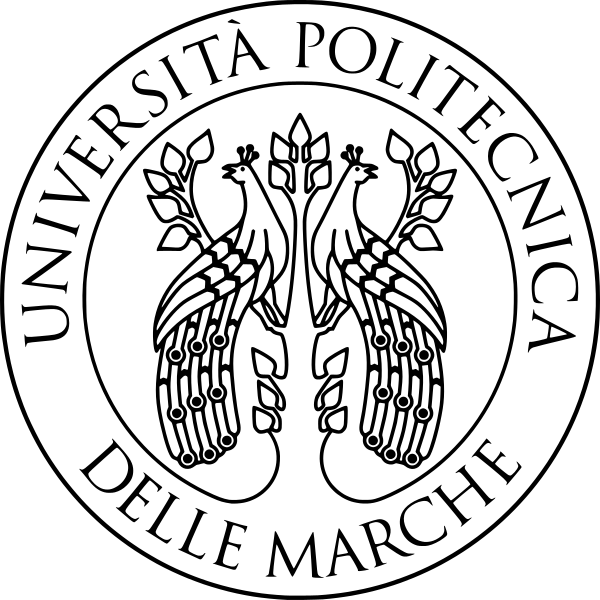
\includegraphics[width=.2\textwidth]{Immagini/univpmlogo}\par\vspace{1cm}
	{\scshape\LARGE Università Politecnica delle Marche\par}
	\vspace{1cm}
	{\scshape\Large Multirate Digital Signal Processing And Adaptive Filter Banks \par}
	\vspace{1.5cm}
	{\huge\bfseries Confronto fra algoritmo LMS e Fast Deconvolution per la cancellazione del crosstalk \par}
	\vspace{2cm}
	{\Large\itshape Matteo Orlandini e Jacopo Pagliuca\par}
	\vfill
	Prof.ssa Stefania \textsc{Cecchi}\\
	Dott.ssa Valeria \textsc{Bruschi}
	
	\vfill
	
	% Bottom of the page
	{\large \today\par}
\end{titlepage}

\thispagestyle{empty}
\tableofcontents

\newpage
\setcounter{page}{1}
\section{Introduzione}
La presente tesina ha lo scopo di riprodurre i risultati ottenuti nel paper \cite{Li:comprehensive_comparison}, il quale mostra un confronto tra l'algoritmo Least Mean Square e Fast Deconvolution per la cancellazione della diafonia.
%che svolge un ruolo importante nell'ascolto di segnali binaurali tramite altoparlanti.

A differenza dei sistemi stereo classici, un sistema audio 3D permette di posizionare i suoni intorno ad un ascoltatore in modo che questi siano percepiti come provenienti da punti arbitrari nello spazio. In questo modo, l'audio 3D può  aumentare il senso di realismo nella musica o nei film e può essere di grande beneficio nella realtà virtuale, nella realtà aumentata, nelle videoconferenze da remoto o per l'intrattenimento casalingo.

La percezione del suono virtuale è ottenuta sintetizzando una coppia di segnali binaurali da un segnale di ingresso monoaurale con le informazioni acustiche 3D fornite: la distanza e la direzione della sorgente sonora rispetto all'ascoltatore. In particolare, il senso dell'orientamento può essere dato dalle funzioni di trasferimento relative alla testa (HRTF), le quali si possono ottenere in modo sperimentale o teorico. Per fornire segnali binaurali, il modo più semplice è attraverso le cuffie. Tuttavia, in molti scenari, ad esempio, a casa o in teleconferenza, molti ascoltatori preferiscono non indossarle. Se vengono utilizzati altoparlanti, la riproduzione di segnali binaurali all'orecchio dell'ascoltatore non è semplice. Ogni orecchio riceve una cosiddetta componente di diafonia, inoltre, i segnali diretti sono distorti dal riverbero della stanza. Per superare i problemi descritti sopra, è necessario un filtro inverso prima di riprodurre il segnale binaurale attraverso gli altoparlanti. 

Poiché occorre invertire i percorsi dell'onda sonora, la cancellazione del crosstalk è un tipico problema di inversione del sistema, che può essere realizzato direttamente o in modo adattivo. Nel primo caso, si presuppone che i percorsi di trasferimento acustico dagli altoparlanti alle orecchie siano noti. %Questi percorsi sono spesso descritti dalle HRTF.

In questo progetto vengono analizzati, implementati e confrontati due algoritmi di cancellazione del crosstalk: LMS (Least Mean Square) e Fast Deconvolution.
Questo viene fatto dapprima tramite degli script in Matlab che poi saranno replicati in C++ utilizzando il software NuTech che permette il processamento dei segnali audio in tempo reale. Per l'implementazione in C++ abbiamo usato le librerie Intel\textsuperscript{\tiny\textregistered} IPP che contengono molte funzioni pronte per l'uso e altamente ottimizzate per diverse architetture Intel\textsuperscript{\tiny\textregistered}~\cite{Intel:IPP}.

La sezione~\ref{sec:Stato_arte} descrive gli algoritmi più comuni in letteratura, mentre la~\ref{sec:Dataset} illustra le funzioni di trasferimento della testa che sono state utilizzate: la loro origine e il significato. Nel capitolo~\ref{sec:descrizione_teorica} è presente la teoria dietro i due algoritmi confrontati. Le sezioni~\ref{sec:codice_matlab} e~\ref{sec:codice_c} presentano e spiegano il codice che è stato sviluppato. Infine i capitoli~\ref{sec:risultati} e~\ref{sec:conclusioni} mostrano i risultati e li confrontano con quelli ottenuti nel paper di riferimento per verificare l'efficacia del codice.
\clearpage

\section{Stato dell'arte}
\label{sec:Stato_arte}    
Il concetto di cancellazione ed equalizzazione della diafonia è stato introdotto da Atal e Schroeder e Bauer nei primi anni Sessanta~\cite{Li:comprehensive_comparison}. Da allora sono stati presentati diversi algoritmi sofisticati per la cancellazione della diafonia, utilizzando due o più altoparlanti, in modo diretto o adattivo. 


Supponendo che i percorsi di trasferimento acustico dagli altoparlanti alle orecchie siano noti, il metodo di implementazione diretto calcola il filtro di cancellazione della diafonia invertendo direttamente le funzioni di trasferimento HRTF. Solitamente viene utilizzato un manichino di una testa con dei microfoni all'interno per stimare queste funzioni.

Il metodo della stima diretta può essere implementato nel dominio del tempo~\cite{Gonzalez:time_domain},~\cite{Mouchtaris:Inverse_filter},~\cite{143434} o della frequenza~\cite{kirkeby:deconvolution_regularization},~\cite{kirkeby:deconvolution_analysis},~\cite{kirkeby:deconvolution_design}. I primi sono generalmente dispendiosi dal punto di vista computazionale, mentre i secondi hanno una complessità inferiore. D'altra parte, gli algoritmi nel dominio del tempo hanno prestazioni migliori di quelli nel dominio della frequenza, data la stessa lunghezza del filtro di cancellazione~\cite{wand:a_stereo_crosstalk}.

Ad esempio, il metodo nel dominio della frequenza chiamato Fast Deconvolution~\cite{kirkeby:deconvolution_regularization},~\cite{kirkeby:deconvolution_analysis},~\cite{kirkeby:deconvolution_design}, che è stato dimostrato essere molto utile e facile da usare in diversi casi pratici, può subire un effetto di convoluzione circolare quando i filtri inversi non sono sufficientemente lunghi rispetto alla durata del percorso acustico.

Nei metodi di implementazione adattivi, il filtro di cancellazione della  diafonia è calcolato adattando i relativi coefficienti usando i segnali di feedback ricevuti da microfoni in miniatura collocati nelle orecchie dell'utente~\cite{Ferrara:FLMS},~\cite{4217047},~\cite{143434},~\cite{wand:a_stereo_crosstalk}. Molti metodi adattativi impiegano tipicamente qualche variazione degli algoritmi LMS o RLS (Recursive Least Squares). L'algoritmo LMS cerca di ridurre una funzione costo $J$ pari all'errore quadratico medio tra il segnale desiderato e l'uscita:
\begin{equation*}
J=E[e[n]^2]=E[(d[n]-y[n])^2],
\end{equation*}
dove $E$ indica il valore medio, $d[n]$ è il segnale desiderato e $y[n]$ è l'uscita del filtro di cancellazione del crosstalk. Questo algoritmo è noto per la sua semplicità e robustezza ed è ampiamente utilizzato, anche se la sua velocità di convergenza è lenta. 

Il metodo LMS non è molto adatto per dati real-time, in quanto per stimare i coefficienti del filtro di cancellazione del crosstalk $h$ usando dati acquisiti in modo continuo si preferiscono metodi ricorsivi~\cite{Ifeachor:DSP}. L'algoritmo RLS si ottiene pesando in modo esponenziale i dati in modo da rimuovere gradualmente gli effetti dei vecchi dati sui coefficienti del filtro e permettere il tracciamento di segnali che variano lentamente. La funzione costo $J$ in questo caso è data da
\begin{equation*}
J(\mathbf{h}_n) = \sum_{i = 0}^{n} \lambda^{n-i}e^2[i],
\end{equation*}
dove $e$ è l'errore definito come la differenza tra il segnale desiderato e l'uscita del filtro di cancellazione del crosstalk e $\mathbf{h}_n$ è il vettore contenente i coefficienti del filtro all'istante $n$. La funzione costo si riduce a quella dell'LMS quando $\lambda = 1$. Il parametro $\lambda$ è chiamato ``forgetting factor'' e viene tipicamente scelto nell'intervallo tra $0.98$ e $1$. 

La funzione costo viene minimizzata facendo la derivata parziale rispetto a tutti i coefficienti $k$ del filtro di cancellazione del crosstalk $h$ e ponendo il risultato pari a zero, come di seguito:
\begin{equation*}
\dfrac{\partial J(\mathbf{h}_n)}{\partial h_n[k]} =  \sum_{i = 0}^{n} 2\lambda^{n-i}e[i]\dfrac{\partial e[i]}{\partial h_n[k]} = - \sum_{i = 0}^{n} 2\lambda^{n-i}e[i]x[i-k] = 0 \quad k = 0, 1, \dots, p,
\end{equation*}
dove $p$ è il numero di coefficienti del filtro $h$. Successivamente, sostituendo $e[i]$ con la definizione di errore si ha:
\begin{equation}\label{eq:RLS}
\dfrac{\partial J(\mathbf{h}_n)}{\partial h_n[k]} = \sum_{i = 0}^{n}\lambda^{n-i}\left[d[i] -\sum_{l=0}^{p} {h_n[l]x[i-l]}\right] x[i-k] = 0 \quad k = 0, 1, \dots, p
\end{equation} 
dove $\sum_{l=0}^{p} {h_n[l]x[i-l]}$ rappresenta l'uscita del filtro $h$ con ingresso $x$. Manipolando l'equazione~\eqref{eq:RLS} si ottiene:
\begin{equation}\label{eq:RLS2}
\sum_{l=0}^{p} {h_n[l]} \left[\sum_{i=0}^{n} \lambda^{n-i}x[i-l]x[i-k]\right] = \sum_{i=0}^{n} \lambda^{n-i} d[i]x[i-k] \quad k = 0, 1,\dots, p.
\end{equation}\label{eq:RLS3}
L'equazione~\eqref{eq:RLS2} si può esprimere in forma matriciale come:
\begin{equation}
\mathbf{R}_x[n]\mathbf{h}_n = \mathbf{r}_{dx}[n],
\end{equation}
dove $\mathbf{R}_x[n]$ è la matrice di covarianza di $x[n]$ e $\mathbf{r}_{dx}[n]$ è la cross-covarianza, o covarianza incrociata, tra $d[n]$ e $x[n]$. Basandoci sull'espressione~\eqref{eq:RLS3} possiamo trovare i coefficienti che minimizzano la funzione costo come:
\begin{equation*}
\mathbf{h}_n = \mathbf{R}^{-1}_x[n]\mathbf{r}_{dx}[n].
\end{equation*}

Occorre ora trovare una forma di soluzione ricorsiva nella forma:
\begin{equation*}
\mathbf{h}_n = \mathbf{h}_{n-1} + \Delta \mathbf{h}_{n-1},
\end{equation*}
dove $\Delta \mathbf{h}_{n-1}$ indica il fattore di correzione all'istante $n-1$. Si può dimostrare che:
\begin{equation*}
\Delta \mathbf{h}_{n-1} = \mathbf{g}[n]\alpha[n],
\end{equation*}
dove:
\begin{equation*}
\mathbf{g}[n] = \mathbf{P}[n-1]\mathbf{x}[n]\left\{\lambda + \mathbf{x}^T[n] \mathbf{P}[n-1] \mathbf{x}[n]\right\}^{-1},
\end{equation*}
in cui:
\begin{equation*}
\mathbf{P}[n] = \mathbf{R}^{-1}_x[n] = \lambda ^ {-1} \mathbf{P}[n-1] -  \mathbf{g}[n]\mathbf{x}^T[n]\lambda^{-1}\mathbf{P}[n-1]
\end{equation*}
e
\begin{equation*}
\alpha[n] = d[n] - \mathbf{x}^T[n]\mathbf{h}_{n-1},
\end{equation*}
dove $\alpha[n]$ è l'\textit{errore a priori}, differente dall'\textit{errore a posteriori} mostrato nella formula seguente:
\begin{equation}
e[n] = d[n] - \mathbf{x}^T[n]\mathbf{h}_{n}.
\end{equation}

Nella derivazione dell'RLS, gli input sono considerati deterministici, mentre per LMS sono stocastici. L'algoritmo RLS può arrivare a convergenza in modo più veloce di LMS, aumentando però il carico computazionale.

Un ulteriore algoritmo derivato da LMS è FLMS (Fast Least Mean Square), descritto in~\cite{Ferrara:FLMS}, viene implementato nel dominio della frequenza e richiede uno sforzo computazionale minore rispetto alla sua controparte nel dominio del tempo. Se l'input del filtro adattativo è un segnale discreto $x_j$, allora l'algoritmo LMS è descritto dalla seguente equazione:
\begin{equation}\label{eq:FLMS1}
\mathbf{h}_{j+1} = \mathbf{h}_j + 2 \mu \epsilon_j \mathbf{x}_j,
\end{equation}
dove $\mathbf{h}_j$ e $\mathbf{x}_j$ sono vettori che rappresentano, rispettivamente, i pesi del filtro e le uscite nella linea di ritardo all'istante $j$, e sono definiti come di seguito:
\begin{equation*}
\begin{split}
\mathbf{h}_j^T = [h_{1,j}, h_{2,j}, \dots, h_{n,j} ]\\
\mathbf{x}_j^T = [x_{j}, x_{j-1}, \dots, x_{j-n+1}].
\end{split} 
\end{equation*}
L'errore $\epsilon_j$ è la differenza tra il segnale desiderato $d_j$ e l'uscita $y_j$, dove $y_j = \mathbf{x}_j^T \mathbf{h}_j$. Per implementare l'equivalente dell'algoritmo LMS in frequenza usando un filtro con $n$ tappi è conveniente dividere il segnale in blocchi da $n$ valori. Durante il $k$-esimo blocco, l'uscita del filtro è data da:
\begin{equation}\label{eq:FLMS2}
y_{kn+i} = \mathbf{x}^T_{kn+i} \mathbf{h}_k	\quad 0 \leq i \leq n-1,
\end{equation}
dove $\mathbf{h}_k$ è il vettore contenente i coefficienti del filtro nel dominio del tempo durante il $k$-esimo blocco. Dopo aver processato il $k$-esimo blocco, il vettore $\mathbf{h}_k$ viene aggiornato iterando l'equazione~\eqref{eq:FLMS1} su $n$ punti come di seguito:
\begin{equation}\label{eq:FLMS3}
\mathbf{h}_{k+1} = \mathbf{h}_k + 2\mu\sum_{i=0}^{n-1}\epsilon_{kn+i}x_{kn+i} = \mathbf{h}_k + 2\mu\nabla_k.
\end{equation}
Le equazioni~\eqref{eq:FLMS2} e~\eqref{eq:FLMS3} possono essere implementate nel dominio della frequenza. Si inizia riscrivendo~\eqref{eq:FLMS2} come convoluzione dei coefficienti del filtro con l'ingresso:
\begin{equation}\label{eq:FLMS4}
y_{kn+j} = \sum_{i=0}^{n-1} h_{i,k}x_{kn+j-i}.
\end{equation}
Per implementare~\eqref{eq:FLMS4} con il metodo \textit{overlap and add} usando la FFT occorre fare un padding di $n$ zeri e usare una FFT a $2n$ punti. Sia $\mathbf{H}_k$ un vettore di lunghezza $2n$ i cui elementi sono i coefficienti nel dominio della frequenza di $\mathbf{h}$ paddati con $n$ zeri:
\begin{equation*}
\mathbf{H}_k^T = \text{FFT}[\mathbf{h}_k^T, 0, \dots, 0].
\end{equation*} 
Sia $\mathbf{X}_k$ la FFT a $2n$ punti del $(k-1)$-esimo e e del $k$-esimo blocco:
\begin{equation*}
\mathbf{X}_k^T = \text{FFT}[x_{(k-1)n}, \dots, x_{kn-1}, x_{kn}, \dots, x_{kn+n-1}].
\end{equation*}
La convoluzione in~\eqref{eq:FLMS4} si realizza calcolando:
\begin{equation}\label{eq:FLMS5}
[y_{kn}, \dots, y_{kn+n-1}]^T = \text{ultimi }n\text{ termini della IFFT di}\left\{\mathbf{H}_k\otimes \mathbf{X}_k\right\} ,
\end{equation}
dove $\otimes$ indica la moltiplicazione elemento per elemento dei vettori $\mathbf{H}_k$ e $\mathbf{X}_k$. L'equazione~\eqref{eq:FLMS5} permette di calcolare i valori dell'uscita del $k$-esimo blocco. Si può osservare che un filtro a $n$ tappi nel dominio del tempo richiede un filtro a $2n$ coefficienti nel dominio della frequenza.

Per implementare l'aggiornamento dei tappi del filtro come mostrato nell'equazione~\eqref{eq:FLMS3} si può scrivere:
\begin{equation*}
\nabla_{j,k} = \sum_{i = 0}^{n-1}\epsilon_{kn+i}x_{kn+i-(j-1)} \quad 1 \leq j \leq n.
\end{equation*}
Determinando l'errore $\mathbf{E}_k$, si può calcolare il valore $\nabla_{k}$ tramite la FFT e un padding di $n$ zeri aggiunti in testa al vettore $\mathbf{E}_k$ come di seguito:
\begin{equation*}
\mathbf{E}_k = \text{FFT} [0, \dots, 0, (d_{kn}-y_{kn}), \dots, (d_{kn+n-1}-y_{kn+n-1})]^T.
\end{equation*}
Successivamente, si calcola:
\begin{equation*}
\nabla_{k} = \text{primi }n\text{ termini della IFFT di}\left\{\mathbf{E}_k\otimes \mathbf{X}^*_k\right\}  ,
\end{equation*}
dove $^*$ indica il complesso coniugato. Infine, vengono calcolati i coefficienti del filtro in frequenza come di seguito:
\begin{equation}\label{eq:FLMS6}
\mathbf{H}_{k+1} = \mathbf{H}_k + 2 \mu \text{ FFT} 
\begin{bmatrix}
\nabla_k\\
0\\
\vdots\\
0
\end{bmatrix},
\end{equation}
con $n$ zeri sotto il vettore $\nabla_k$. Se gli ultimi $n$ valori della IFFT dei coefficienti iniziali di $\mathbf{H}_0$ sono forzati a zero, allora l'equazione~\eqref{eq:FLMS6} è l'implementazione esatta di~\eqref{eq:FLMS3} nel dominio della frequenza.

Per ognuno degli $n$ valori del blocco, l'algoritmo FLMS richiede cinque FFT a $2n$ punti e due moltiplicazioni complesse a $2n$ punti. Per ingressi reali, le trasformate sono simmetriche, quindi richiedono il calcolo solamente dei primi $n+1$ punti. Assumendo che una moltiplicazione complessa sia equivalente a quattro moltiplicazioni reali, si può dimostrare il seguente rapporto:
\begin{equation}\label{eq:FLMS7}
\dfrac{\text{Moltiplicazioni reali FLMS}}{\text{Moltiplicazioni reali LMS}} = \dfrac{5\left(\log\dfrac{n}{2}\right)+14}{n}.
\end{equation}
Per $n \geq 64$ il rapporto~\eqref{eq:FLMS7} diventa minore di 1, quindi le moltiplicazioni reali dell'algoritmo LMS sono maggiori di quelle di FLMS.

Sebbene molti algoritmi siano stati proposti, il metodo adattativo viene usato più in ambito accademico che nella vita di tutti i giorni. Il motivo è che le persone che non vogliono usare le cuffie probabilmente non vorrebbero utilizzare neanche un paio di microfoni nelle orecchie per ottimizzare la riproduzione degli altoparlanti. Una limitazione di un sistema di cancellazione della diafonia nasce dal fatto che ogni movimento dell'ascoltatore che supera i $75-100$ \si{\milli \meter} può cambiare completamente l'effetto desiderato. Questo problema può essere risolto seguendo in tempo reale la testa dell'ascoltatore nello spazio 3D~\cite{Bai:objective_analysis},~\cite{Kyriakakis:fundamental_technological_limitations}. La posizione della testa viene determinata da un localizzatore magnetico o basato su fotocamera, quindi i filtri HRTF e quelli di cancellazione della diafonia sono aggiornati in tempo reale in base alla posizione dell'ascoltatore. In questo caso, il filtro di cancellazione della diafonia richiede un'elevato sforzo computazionale per essere aggiornato in tempo reale in base alla posizione della testa~\cite{wand:a_stereo_crosstalk}. 

In acustica, la deconvoluzione a singolo canale è particolarmente utile poiché può compensare la risposta di trasduttori imperfetti come cuffie, altoparlanti e amplificatori. La deconvoluzione multicanale è necessaria nella progettazione di sistemi di cancellazione della diafonia e sistemi di imaging di sorgenti virtuali.%~\cite{kirkeby:deconvolution_analysis} 

La Fast Deconvolution è un metodo molto veloce per calcolare una matrice di filtri digitali che può essere utilizzata per controllare le uscite di un impianto multicanale. Questo metodo è tipicamente più veloce di diversi ordini di grandezza rispetto ai metodi nel dominio del tempo e combina i principi dell'inversione dei minimi quadrati nel dominio della frequenza e il metodo di regolarizzazione di ordine zero. I metodi di regolarizzazione rinunciano a trovare la soluzione esatta del problema, calcolando invece la soluzione di un problema leggermente diverso ma meglio condizionato. %~\cite{kirkeby:deconvolution_regularization}

L'algoritmo presuppone che sia possibile utilizzare filtri ottimali lunghi, e funziona bene solo quando il parametro di regolarizzazione è impostato in modo appropriato. Nella pratica questo parametro viene determinato per tentativi.%~\cite{kirkeby:deconvolution_design}

Una tipica situazione di ascolto con due altoparlanti con cancellazione del closstalk è rappresentata in figura~\ref{fig:head}. La rappresentazione in frequenza dei segnali desiderati binaurali è indicata con $X_1$ e $X_2$ per i suoni che raggiungono rispettivamente orecchio destro e sinistro.
Con $Y_1$ e $Y_2$ invece, si indicano i suoni che effettivamente raggiungono l'ascoltatore, attraversando il sistema. $C_{i, j}$ sono le HRTF dagli altoparlanti alle orecchie dell'ascoltatore, $H_{i,j}$ sono i filtri di cancellazione della diafonia, per $i , j =1,2$.
\begin{figure}[h]
	\centering	
	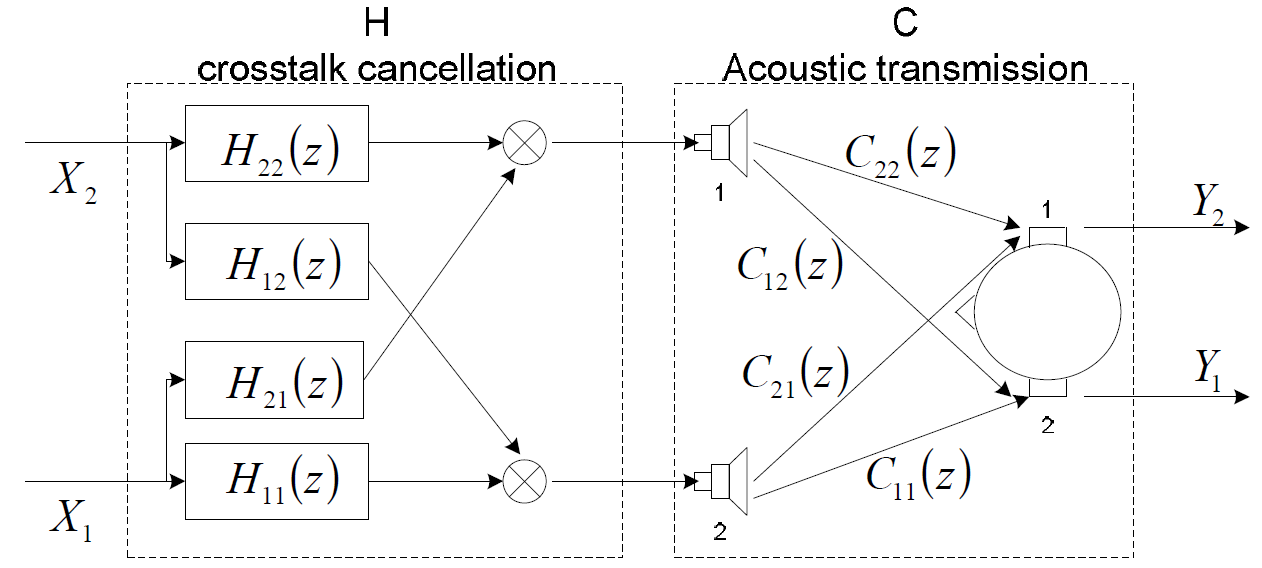
\includegraphics[width=1\textwidth]{Immagini/head}
	\caption{Diagramma a blocchi del sistema sonoro usato}
	\label{fig:head}
\end{figure}

Il sistema illustrato in figura~\ref{fig:head} può essere rappresentato nel dominio della frequenza come:
\begin{equation}\label{eq:Y=CHX}
\textbf{Y} = \textbf{CHX}
\end{equation}
ovvero:
\begin{equation}\label{eq:sistema_sonoro}
\begin{bmatrix}
Y_1\\
Y_2
\end{bmatrix}
=
\begin{bmatrix}
C_{11} & C_{12}\\
C_{21} & C_{22}
\end{bmatrix}
\begin{bmatrix}
H_{11} & H_{12}\\
H_{21} & H_{22}
\end{bmatrix}
\begin{bmatrix}
X_1\\
X_2
\end{bmatrix}
\end{equation}
L'equazione~\eqref{eq:sistema_sonoro} può essere riscritta come:
\begin{equation}
\begin{bmatrix}
Y_1\\
Y_2
\end{bmatrix}
=
\begin{bmatrix}
C_{11} X_1 & C_{12} X_1 & C_{11} X_2 & C_{12} X_2 \\ 
C_{21} X_1 & C_{22} X_1 & C_{21} X_2 & C_{22} X_2 \\ 
\end{bmatrix}
\begin{bmatrix}
H_{11}\\
H_{21}\\
H_{12}\\
H_{22}\\
\end{bmatrix}
\end{equation}
Per avere il segnale in uscita uguale a quello desiderato $H$ dovrebbe essere l'inversa di $C$. La diretta inversa di $C$ però non garantisce la cancellazione del crosstalk in quanto gli elementi potrebbero non soddisfare la condizione di fase minima. 
\clearpage

\section{Dataset}
\label{sec:Dataset}
Il dataset usato è composto ad un ampio set di misurazioni della funzione di trasferimento relativa alla testa (HRTF) di un microfono dummy-head KEMAR. Le misurazioni consistono nelle risposte impulsive dell'orecchio sinistro e destro di un altoparlante Realistic Optimus Pro 7 montato a 1,4 metri dal KEMAR. Sono state utilizzate sequenze binarie pseudo-casuali per ottenere le risposte impulsive a una frequenza di campionamento di \SI{44.1}{\kilo \hertz}~\cite{Gardner:HRTF}. 

Le misurazioni sono state effettuate nella camera anecoica del MIT. Il KEMAR è stato montato in posizione verticale su un giradischi motorizzato che può essere ruotato con precisione sotto il controllo del computer. L'altoparlante è stato montato su un supporto a braccio che ha consentito il posizionamento accurato dell'altoparlante a qualsiasi elevazione rispetto al KEMAR. Pertanto, le misurazioni sono state effettuate un'elevazione alla volta, impostando l'altoparlante all'altezza corretta e quindi ruotando il KEMAR su ciascun azimut.

I dati HRTF vengono archiviati nelle directory per elevazione. Ogni nome di directory ha il formato ``elevEE'', dove ``EE'' è l'angolo di elevazione. All'interno di ogni directory, il nome di ogni file ha il formato ``XEEeAAAa.wav'' dove X può essere ``L'' o ``R'' rispettivamente per la risposta dell'orecchio sinistro e destro, ``EE'' è l'angolo di elevazione della sorgente in gradi, da -40° a 90°, e ``AAA'' è l'azimut della sorgente in gradi, da 0° a 355°. Gli angoli di elevazione e azimut indicano la posizione della sorgente rispetto al KEMAR, in modo che, ad esempio, in corrispondenza dell'elevazione 0 e azimut 0 sia di fronte al KEMAR , l'elevazione 90 è direttamente sopra il KEMAR, elevazione 0 e azimut 90 è a destra del KEMAR. Ad esempio, il file ``R-20e270a.wav'' è la risposta dell'orecchio destro, con la sorgente 20 gradi sotto il piano orizzontale e 90 gradi a sinistra della testa.
\clearpage
\section{Descrizione teorica degli algoritmi}
\label{sec:descrizione_teorica}
\subsection{LMS}
\label{subsec:LMS_teoria}
Per la cancellazione del crosstalk l'algoritmo più comune è quello dell'LMS che nonostante sia semplice e accurato, ha una veloce convergenza~\cite{143434},~\cite{4217047}. La figura~\ref{fig:lms} mostra il diagramma di cancellazione del crosstalk usando LMS, $x$ indica l'ingresso, $y$ l'uscita, $d$ il segnale desiderato ed $e$ l'errore.

\begin{figure}[h]
	\centering	
	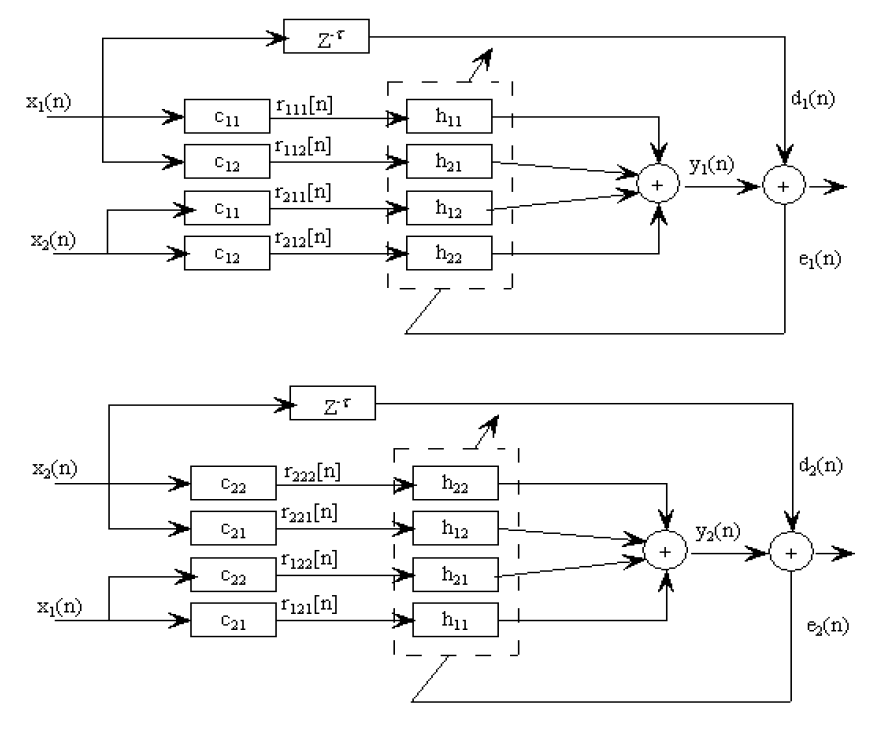
\includegraphics[width=\textwidth]{Immagini/lms.png}
	\caption{Diagramma a blocchi della cancellazione del crosstalk usando LMS}
	\label{fig:lms}
\end{figure}

Le variabili con lettera minuscola rappresentano il segnale nel dominio del tempo e $\tau$ rappresenta il ritardo del sistema. Per sistemi causali, l'uscita $y_i[n]$ dovrebbe essere idealmente una versione ritardata dell'ingresso $x_i[n]$. Le sequenze $r_{ilm}$ sono i segnali $x_i[n]$ di ingresso filtrati dalle funzioni $c_{lm}$ che hanno $M$ tappi nel dominio del tempo.

In generale, si può scrivere l'uscita $y[n]$ del filtraggio nell'$n$-esimo istante di un segnale $\mathbf{a[n]}$ definito come:
\begin{equation*}
\mathbf{a[n]} = \left[a[n], a[n-1], \dots, a[n - M + 1]\right]^T
\end{equation*}
con un filtro $\mathbf{b[n]}$ di lunghezza $M$ con coefficienti del tipo:
\begin{equation*}
\mathbf{b[n]} =  \left[b_{0}[n], b_{1}[n], \dots,\\ b_{M-1}[n]\right]^T
\end{equation*}
come:
\begin{equation}\label{eq:filtraggio_prodotto_scalare}
y[n] = \sum_{j=0}^{M-1}b_{j}[n]a[n-j] = \mathbf{b}^T[\mathbf{n}] \cdot \mathbf{a}[\mathbf{n}].
\end{equation}

Il filtraggio dei segnali di riferimento $x_i[n]$ con le hrir $c_{lm}$ è dato dalla seguente equazione
\begin{equation}\label{eq:r_ilm}
r_{ilm}[n]=\sum_{j=0}^{M-1}c_{lm}[j]x_i[n-j].
\end{equation}

Si può applicare la formula~\eqref{eq:filtraggio_prodotto_scalare} all'equazione~\eqref{eq:r_ilm} per calcolare le $r_{ilm}[n]$ nel seguente modo:

\begin{equation}\label{eq:r_ilm_prodotto_scalare}
r_{ilm}[n]=\sum_{j=0}^{M-1}c_{lm,j}[n]x_i[n-j] = \mathbf{c_{lm}}^T[\mathbf{n}] \cdot \mathbf{x_i}[\mathbf{n}].
\end{equation}

Il segnale ricevuto ad ogni orecchio è dato da:
\begin{equation}\label{eq:y_i_lms}
y_i[n]=r_{1i1}[n] \circledast h_{11}[n]+r_{1i2}[n] \circledast h_{21}[n]+
r_{2i1}[n] \circledast h_{12}[n]+r_{2i2}[n] \circledast h_{22}[n]
\end{equation}
dove $i,l,m$ assumono i valori 1 o 2 e $\circledast$ rappresenta la convoluzione. Il criterio dell'algoritmo LMS è la minimizzazione della funzione costo
\begin{equation}\label{eq:errore_lms}
J=E[e[n]^2]=E[(d[n]-y[n])^2]
\end{equation}
dove $e[n]$, $d[n]$ e $y[n]$ sono definiti come
\begin{equation}
e[n]=
\begin{bmatrix}
e_1[n]\\
e_2[n]
\end{bmatrix},\quad
d[n]=
\begin{bmatrix}
d_1[n]\\
d_2[n]
\end{bmatrix},\quad
y[n]=
\begin{bmatrix}
y_1[n]\\
y_2[n]
\end{bmatrix}
\end{equation}
La minimizzazione di $J$ avviene con il metodo steepest descend.
Nel dominio del tempo discreto il sistema si può scrivere come
\begin{equation}\label{eq:y_lms}
\begin{bmatrix}
	y_1[n]     \\
	y_2[n]    
\end{bmatrix}
= 
\begin{bmatrix}
	c_{11}[n] \circledast x_1[n]  &  c_{12}[n] \circledast x_1[n]  & c_{11}[n] \circledast x_2[n]  & c_{12}[n] \circledast x_2[n]    \\
	c_{21}[n] \circledast x_1[n]  &  c_{22}[n] \circledast x_1[n]  & c_{21}[n] \circledast x_2[n]  & c_{22}[n] \circledast x_2[n]     
\end{bmatrix} 
\circledast
\begin{bmatrix}
	h_{11}[n] \\
	h_{21}[n] \\
	h_{12}[n] \\
	h_{22}[n]  
\end{bmatrix}
\end{equation}
Usando~\eqref{eq:r_ilm}, l'equazione~\eqref{eq:y_lms} diventa
\begin{equation}\label{eq:y_lms2}
\begin{bmatrix}
	y_1[n]     \\
	y_2[n]    
\end{bmatrix}
= 
\begin{bmatrix}
	r_{111}[n]  &	r_{112}[n]  &  r_{211}[n]  &	r_{212}[n]    \\
	r_{121}[n]  &	r_{122}[n]  &  r_{221}[n]  &	r_{222}[n]    \\
\end{bmatrix} 
\circledast
\begin{bmatrix}
	h_{11}[n] \\
	h_{21}[n] \\
	h_{12}[n] \\
	h_{22}[n]  
\end{bmatrix} 
\end{equation}
Per ottenere l'errore si calcola la differenza fra il segnale desiderato è l'uscita effettiva.
\[
e_1^{(1)} = d_1 - (r_{111} \circledast h_{11} + r_{112} \circledast h_{21} + r_{211} \circledast h_{12} + r_{212} \circledast h_{22})
\]
l'aggiornamento avviene come di seguito:
\begin{equation}\label{eq:aggiornamento_lms}
h^{(k+1)} = h^{(k)} - \mu e_i^{(k)} \cdot \mathbf{r}_i^T
\end{equation}
dove $\mathbf{r}_i$ è l'i-esima riga della matrice che contiene le $r_{ilm}$ nell'equazione~\eqref{eq:y_lms2} e $e_i^{(k)}$ è l'errore k-esimo step e all'i-esima riga. Esplicitando l'equazione~\eqref{eq:aggiornamento_lms}, si ottiene
\[
\begin{split}
h_{11}^{(k+1)}[n] \leftarrow h_{11}^{(k)}[n] - \mu e_1^{(1)} \cdot r_{111}[n]\\
h_{21}^{(k+1)}[n] \leftarrow h_{21}^{(k)}[n] - \mu e_1^{(1)} \cdot r_{112}[n]\\
h_{12}^{(k+1)}[n] \leftarrow h_{12}^{(k)}[n] - \mu e_1^{(1)} \cdot r_{211}[n]\\
h_{22}^{(k+1)}[n] \leftarrow h_{22}^{(k)}[n] - \mu e_1^{(1)} \cdot r_{212}[n]
\end{split}
\]
Allo stesso modo, per il secondo canale l'errore è definito come:
\[e_2^{(2)} = d_2- (r_{121} \circledast h_{11} + r_{122} \circledast h_{21} + r_{221} \circledast h_{12} + r_{222} \circledast h_{22})
\]

\[
\begin{split}
h_{11}^{(k+1)}[n] \leftarrow h_{11}^{(k)}[n] - \mu e_2^{(2)} \cdot r_{121}[n]\\
h_{21}^{(k+1)}[n] \leftarrow h_{21}^{(k)}[n] - \mu e_2^{(2)} \cdot r_{122}[n]\\
h_{12}^{(k+1)}[n] \leftarrow h_{12}^{(k)}[n] - \mu e_2^{(2)} \cdot r_{221}[n]\\
h_{22}^{(k+1)}[n] \leftarrow h_{22}^{(k)}[n] - \mu e_2^{(2)} \cdot r_{222}[n]\\
\end{split}
\]

\subsection{Fast Deconvolution}
\label{subsec:FD_teoria}
La deconvoluzione~\cite{kirkeby:deconvolution_regularization}~\cite{kirkeby:deconvolution_analysis}~\cite{kirkeby:deconvolution_design}, nella sua forma più elementare, può essere descritta come il compito di calcolare l'input di un sistema a tempo discreto conoscendo il suo output. Di solito si presume che il sistema sia lineare e che la relazione input output sia nota con precisione. 
%In acustica e audio, la deconvoluzione a singolo canale è particolarmente utile poiché può compensare la risposta di trasduttori imperfetti come cuffie, altoparlanti e amplificatori. La deconvoluzione multicanale è necessaria nella progettazione di sistemi di cancellazione della diafonia e sistemi di imaging di sorgenti virtuali.%~\cite{kirkeby:deconvolution_analysis}
%Nel progetto siamo interessati alle tecniche di deconvoluzione allo scopo di progettare filtri digitali per la riproduzione del suono su due canali. Più specificamente, dato un set di altoparlanti S, l'obiettivo è riprodurre un campo sonoro desiderato nei punti R dello spazio nel modo più accurato possibile. Questo principio è applicato dai cosiddetti sistemi di cancellazione della diafonia che vengono utilizzati per riprodurre registrazioni binaurali su due altoparlanti. In questo caso, viene utilizzata una matrice $2 \times 2$ di filtri digitali per compensare sia la risposta ambientale che la risposta degli altoparlanti, e anche per annullare la diafonia dall'altoparlante sinistro all'orecchio destro e viceversa. Un problema correlato è quello di ottenere una perfetta ``dereverberazione'' della risposta di una stanza in una posizione del microfono utilizzando due filtri digitali per calcolare l'ingresso a due altoparlanti. La fast deconvolution un metodo molto veloce per calcolare una matrice di filtri digitali che può essere utilizzata per controllare le uscite di un impianto multicanale. Questo metodo è tipicamente più veloce di diversi ordini di grandezza rispetto ai metodi nel dominio del tempo. Combina i principi dell'inversione dei minimi quadrati nel dominio della frequenza e il metodo di regolarizzazione di ordine zero che viene tradizionalmente utilizzato quando ci si trova di fronte a un problema di inversione mal condizionata.%~\cite{kirkeby:deconvolution_regularization}
%La regolarizzazione dipendente dalla frequenza viene utilizzata per prevenire picchi elevati nella risposta in ampiezza dei filtri ottimali. Un ritardo di modellazione viene utilizzato per garantire che la rete di cancellazione del cross-talk funzioni bene non solo in termini di ampiezza, ma anche in termini di fase. L'algoritmo presuppone che sia possibile utilizzare filtri ottimali lunghi, e funziona bene solo quando due parametri di regolarizzazione, un fattore di forma e un fattore di guadagno, sono impostati in modo appropriato. In pratica, i valori dei due parametri di regolarizzazione sono determinati più facilmente da esperimenti per tentativi.%~\cite{kirkeby:deconvolution_design}
Consideriamo una funzione costo del tipo
\begin{equation}\label{eq:funzione_costo_fd}
J = E + \beta V(f)
\end{equation}
dove $E$ è una misura dell'errore della pressione sonora
\begin{equation}\label{eq:errore_fd}
E = | Y_1 - X_1 |^2  + | Y_2 - X_2 |^2
\end{equation}
e $V$ è una funzione della frequenza che indica il costo computazionale. Il numero $\beta \geq 0$ è un parametro di regolarizzazione che determina quanto peso
assegnare alla funzione $V$. La regolarizzazione dipendente dalla frequenza viene utilizzata per prevenire picchi elevati nella risposta in ampiezza dei filtri ottimali. Poiché non sappiamo a priori se la matrice $C$ è non singolare per determinate frequenze, la matrice $H$ di cancellazione del crosstalk può contenere valori molto alti. All'aumentare di $\beta$ da zero a infinito, $J$ cambia gradualmente dalla minimizzazione della sola funzione di errore $E$ alla minimizzazione dello sforzo computazionale $V$.

Siano $S$ i segnali trasferiti agli altoparlanti facendo passare il segnale $X$ attraverso la matrice di cancellazione del crosstalk $H$. Otteniamo
\begin{equation}
V(f) = S_b ^{+} S_b
\end{equation}
con
\begin{equation}
S_b = BS = BHX
\end{equation}
dove $B$ è una matrice $2 \times 2$ e il simbolo $^+$ indica l'inversa generalizzata della matrice $S_b$. La soluzione approssimata della funzione $J$ è definita da 
\begin{equation}\label{eq:H_FD}
H(z) = \left[C^T (z^{-1}) C(z) + \beta B^T B)\right]^{-1} C^T(z^{-1})
\end{equation}
dove l'apice $^T$ denota la trasposta della matrice. Se la matrice $B$ è uguale alla matrice identità $I$, si ottiene $S_b = S$, dunque l'equazione~\eqref{eq:H_FD} diventa
\begin{equation}\label{eq:H_FD2}
H(z) = \left[C^T (z^{-1}) C(z) + \beta I)\right]^{-1} C^T(z^{-1}) z^{-m}
\end{equation}
dove la componente $z^{-m}$ implementa un ritardo di $m$ campioni. Un ritardo di modellazione viene utilizzato per garantire che la rete di cancellazione del cross-talk funzioni bene non solo in termini di ampiezza, ma anche in termini di fase.

Le equazioni~\eqref{eq:H_FD} e~\eqref{eq:H_FD2} rappresentano una espressione di $H(z)$ nel dominio continuo della frequenza. Se, come nel nostro caso, il dominio della frequenza è discreto, occorre usare la formula~\eqref{eq:H_FD3}, in cui il valore di $H[k]$ è dato da
\begin{equation}\label{eq:H_FD3}
H[k] = \left[C^H[k] C[k] + \beta I)\right]^{-1} C^H[k]
\end{equation}
dove $k$ indica la $k$-esima frequenza corrispondente a $\exp(j2\pi k/N)$ e l'apice~$^H$ denota l'operatore Hermitiano che fa la trasposta coniugata del suo argomento. Dall'equazione si può osservare che ponendo $\beta = 0$ si ottiene $H = C^{-1}$. In questo caso, poiché $Y = CHX = C C^{-1} X = IX = X$, si ottiene in uscita il segnale d'ingresso.

L'equazione~\eqref{eq:H_FD3} si ricava dalla~\eqref{eq:H_FD2} notando che la trasformata di Fourier a tempo discreto è la valutazione della trasformata zeta sul cerchio unitario, quindi ponendo $z = e^{j\omega}$ si ottiene la DTFT. Si noti che un generico segnale $X(z^{-1}) = X(e^{-j\omega}) = X^*(e^{j\omega})$ corrisponde nel dominio discreto della frequenza a $X^*[k]$ e nel tempo discreto all'inversione temporale $x[-n]$. Come precedentemente detto, l'operatore Hermitiano fa la trasposta coniugata del suo argomento, quindi si può capire perché $C^T(z^{-1})$ diventa $C^H[k]$ nell'equazione~\eqref{eq:H_FD3}.

Il ritardo di $m$ campioni $z^{-m}$ viene esplicitato nella risposta impulsiva che viene calcolata implementando i seguenti passi:
\begin{enumerate}
\item si calcola la matrice $2 \times 2$ $C[k]$ tramite una FFT delle risposte impulsive $c_{ij}[n]$ con $i = 1, 2$ e $j = 1, 2$. Ad esempio, $C_{11}[k]$ contiene l'ampiezza della $k$-esima armonica della FFT di $c_{11}$,
\item si calcola $H[k]$ usando la formula~\eqref{eq:H_FD3},
\item si calcola $h[n]$ facendo una FFT inversa a $N$ punti,
\item si implementa uno shift ciclico di $m$ campioni per ogni elemento di $h_{ij}[n]$ con $i = 1, 2$ e $j = 1, 2$.
\end{enumerate}

Dato che l'uscita $Y$ è data da
\begin{equation}\label{eq:y_matrix}
Y = CHX = 
\begin{bmatrix}
C_{11} X_1 & C_{12} X_1 & C_{11} X_2 & C_{12} X_2 \\ 
C_{21} X_1 & C_{22} X_1 & C_{21} X_2 & C_{22} X_2 \\ 
\end{bmatrix}
\begin{bmatrix}
H_{11}\\
H_{21}\\
H_{12}\\
H_{22}\\
\end{bmatrix}
\end{equation}
nell'implementazione pratica non si può calcolare tutta l'uscita con la sola operazione matriciale~\eqref{eq:y_matrix}, occorre usare la tecnica dell'overlap and save per filtrare l'ingresso $X$ con i filtri $C$ e $H$. L'overlap and save è utile per eseguire un filtraggio in real time con un filtro a risposta impulsiva finita. Questa tecnica viene usata per fare la convoluzione a blocchi tra un segnale di ingresso $x[n]$ molto lungo e un filtro FIR $h[n]$:
\begin{equation}
y[n] = x[n] * h[n] = \sum_{m=-\infty}^{+\infty} {h[m] \cdot x[n-m]} = \sum_{m=1}^{M} {h[m] \cdot x[n-m]}
\end{equation}
poiché $h[m] \neq 0$ solo per $m \in [1, M]$.

L'overlap and save permette di calcolare dei blocchi di $y[n]$ di lunghezza $L$ e concatenarli insieme per formare il segnale di uscita completo. Si definisce il $k$-esimo blocco d'ingresso come
\begin{equation}
x_k[n] = 
\begin{cases}
x[n+kL], & 1 \leq n \leq L + M - 1\\
0 & \text{altrove}
\end{cases}
\end{equation}
quindi il $k$-esimo blocco di uscita è dato da 
\begin{equation}
y_k[n] = x_k[n] * h[n] = \sum_{m=1}^{M} {h[m] \cdot x_k[n-m]}.
\end{equation}
Si può definire l'uscita per $kL + M \leq n \leq KL + L +M - 1$, o in modo equivalente per $M \leq n - kL \leq L + M - 1$, nel seguente modo:
\begin{equation}
y[n] = \sum_{m=1}^{M} {h[m] \cdot x_k[n-kL-m]} = y_k[n - kL].
\end{equation}
L'implementazione dell'overlap and save con un filtro composto da $(L + M - 1)$ tappi consiste nei seguenti passi:
\begin{enumerate}
\item si divide il segnale di ingresso in blocchi di lunghezza $L$
\item nel caso del primo blocco si aggiungono $M - 1$ zeri all'inizio, altrimenti si aggiungono all'inizio del blocco gli ultimi $M - 1$ campioni del blocco precedente, come mostrato in figura~\ref{fig:ols},
\item si fa la FFT a $L + M - 1$ punti del $k$-esimo blocco di ingresso,
\item si fa la FFT a $L + M - 1$ punti del filtro FIR $h[n]$
\item si moltiplicano le FFT calcolate per trovare la risposta in frequenza del $k$-esimo blocco di uscita,
\item si fa la FFT inversa a $L + M - 1$ punti del $k$-esimo blocco di uscita,
\item si scartano i primi $M - 1$ punti, ottenendo il $k$-esimo blocco in uscita di lunghezza $L$, come mostrato nei blocchi di uscita $y_k$ di figura~\ref{fig:ols}.
\end{enumerate}

Un'implementazione più efficiente è invece quella descritta di seguito e mostrata nella figura~\ref{fig:ols_digramma}, in cui i primi due punti precedentemente elencati rimangono uguali:
\begin{enumerate}\setcounter{enumi}{2}
\item si fa la FFT a $2 \cdot (L + M - 1)$ punti del $k$-esimo e del $(k-1)$-esimo blocco di ingresso lunghi rispettivamente $(L + M - 1)$ campioni,
\item si fa la FFT a $2 \cdot (L + M - 1)$ punti del filtro FIR $h[n]$ con un padding di $(L + M - 1)$ zeri
\item si moltiplicano le FFT calcolate per trovare la FFT del blocco di uscita,
\item si fa la FFT inversa del blocco di uscita,
\item si scartano i primi $L + M - 1$ punti nel tempo dell'uscita.
\end{enumerate}

\begin{figure}[h]
	\centering	
	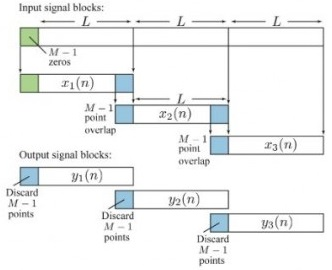
\includegraphics[width=.5\textwidth]{Immagini/ols}
	\caption{Metodo Overlap and Save}
	\label{fig:ols}
\end{figure}

\begin{figure}[h]
	\centering	
	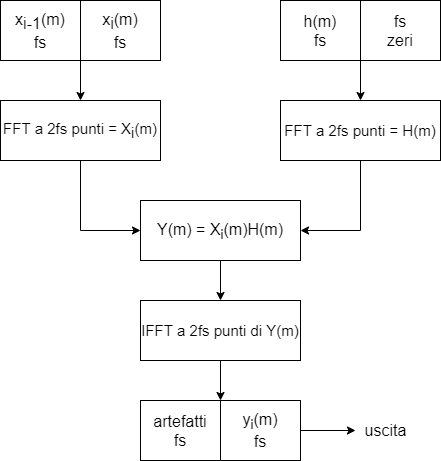
\includegraphics[width=.5\textwidth]{Immagini/ols_diagram}
	\caption{Diagramma dell'implementazione dell'Overlap and Save}
	\label{fig:ols_digramma}
\end{figure}

\clearpage

\section{Codice Matlab}
\label{sec:codice_matlab}
\subsection{LMS}
\label{subsec:codice_matlab_lms}
Nel codice dell'algoritmo LMS in Matlab si carica il file audio in formato wav ``Daft Punk - Get Lucky\_cut.wav''. Poiché questo formato contiene i campioni del canale sinistro e di quello destro, si dividono i due canali salvando il primo nella variabile \texttt{x1} e il secondo in \texttt{x2}.

\begin{lstlisting}[label=code:caricamento_audio_lms, caption=Caricamento del file audio, captionpos=b]
[x, Fsample] = audioread('Daft Punk - Get Lucky_cut.wav');
x1 = x(:, 1);
x2 = x(:, 2);
\end{lstlisting}

Allo stesso modo vendono caricate le quattro HRIR \texttt{c11}, \texttt{c12}, \texttt{c21} e \texttt{c22}.

\begin{lstlisting}[label=code:caricamento_hrir_lms, caption=Caricamento delle HRIR, captionpos=b]
% c11: HRIR left loudspeaker - left ear
[c11,Fs] = audioread('HRTF_measurements/elev0/L0e330a.wav'); 
% c12: HRIR right loudspeaker - left ear
[c12,~] = audioread('HRTF_measurements/elev0/L0e030a.wav');     
% c21: HRIR left loudspeaker - right ear
[c21,~] = audioread('HRTF_measurements/elev0/R0e330a.wav');    
% c22: HRIR right loudspeaker - righ ear
[c22,~] = audioread('HRTF_measurements/elev0/R0e030a.wav');  
\end{lstlisting}

Viene salvata la lunghezza dei filtri $c_{11}$, $c_{12}$, $c_{21}$ e $c_{22}$ nella variabile \texttt{M}. Si ha che $M = 512$ e si imposta il ritardo temporale \texttt{tau} pari a \texttt{M}. Conoscendo il valore del ritardo temporale, è possibile costruire i due segnali desiderati \texttt{d1} e \texttt{d2} mettendo \texttt{tau} zeri all'inizio del vettore d'ingresso.

\begin{lstlisting}[label=code:segnale_desiderato_lms, caption=Costruzione del segnale desiderato, captionpos=b]
M = length(c11);      % lunghezza dei filtri c11, c12, c21, c22
% il segnale desiderato e' x ritardato di tau campioni
tau = M;   % ritardo temporale
d1 = [zeros(tau,1); x1(1:end-tau)]; % segnale desiderato 1 (left)
d2 = [zeros(tau,1); x2(1:end-tau)]; % segnale desiderato 2 (right)
\end{lstlisting}

Vengono inizializzati i vettori \texttt{y1} e \texttt{y2} di uscita, i vettori \texttt{e1} e \texttt{e2} che contengono l'errore per i due canali, i vettori \texttt{r\ped{ilm}} che contengono il filtraggio di \texttt{x1} e \texttt{x2} con \texttt{c11}, \texttt{c12}, \texttt{c21} e \texttt{c22}. Questi vettori sono tutti di lunghezza pari a quella del segnale x, cioè \texttt{L}.

\begin{lstlisting}[label=code:inizializzazione_vettori_L, caption=Inizializzazione dei vettori di lunghezza L, captionpos=b]
L = length(x1);
y1 = zeros(L,1);  % output 1 (left)
y2 = zeros(L,1);  % output 2 (right)

e1 = zeros(L,1);  % errore 1 (left)
e2 = zeros(L,1);  % errore 2 (right)

r111 = zeros(L,1);    % uscita di x1 filtrato da c11 per output y1
r112 = zeros(L,1);    % uscita di x1 filtrato da c12 per output y1
r211 = zeros(L,1);    % uscita di x2 filtrato da c11 per output y1
r212 = zeros(L,1);    % uscita di x2 filtrato da c12 per output y1
r222 = zeros(L,1);    % uscita di x2 filtrato da c22 per output y2
r221 = zeros(L,1);    % uscita di x2 filtrato da c21 per output y2
r122 = zeros(L,1);    % uscita di x1 filtrato da c22 per output y2
r121 = zeros(L,1);    % uscita di x1 filtrato da c21 per output y2
\end{lstlisting}

Successivamente, vengono inizializzati i vettori di lunghezza \texttt{M}, le variabili \texttt{h11},  \texttt{h12},  \texttt{h21} e  \texttt{h22} contengono i filtri di ricostruzione, i buffer \texttt{x1buff} e \texttt{x2buff} necessari per il filtraggio con i c e i buffer delle uscite $r_{ilm}$ dove $i, l, m = 0,1$.

\begin{lstlisting}[label=code:inizializzazione_vettori_M, caption=Inizializzazione dei vettori di lunghezza M, captionpos=b]
x1buff = zeros(M, 1);
x2buff = zeros(M, 1);

r111buff = zeros(M,1);    
r112buff = zeros(M,1);    
r211buff = zeros(M,1);  
r212buff = zeros(M,1);    
r222buff = zeros(M,1);    
r221buff = zeros(M,1);    
r122buff = zeros(M,1);   
r121buff = zeros(M,1);  
\end{lstlisting}

Nel codice~\ref{code:filtraggio_x_c} viene usato un $\mu = 10^{-3}$ e viene implementata l'equazione~\eqref{eq:r_ilm_prodotto_scalare} che effettua il filtraggio tra le hrir e il segnale di ingresso. Per fare questo, si utilizza un buffer che aggiunge in testa il campione entrante invertendo il segnale di ingresso. Facendo il prodotto scalare dei buffer di ingresso con le rispettive $c_{lm}$, si ottiene il filtraggio desiderato.

\begin{lstlisting}[label=code:filtraggio_x_c, caption=Filtraggio del segnale di ingresso con le hrir, captionpos=b]
mu = 1e-3; 
for n = 1:L
    x1buff = [x1(n); x1buff(1:end-1)];
    x2buff = [x2(n); x2buff(1:end-1)];
   
    r111(n) = c11'*x1buff;
    r112(n) = c12'*x1buff;
    r211(n) = c11'*x2buff;
    r212(n) = c12'*x2buff;
    r222(n) = c22'*x2buff;
    r221(n) = c21'*x2buff;
    r122(n) = c22'*x1buff;
    r121(n) = c21'*x1buff;
\end{lstlisting}

L'equazione~\eqref{eq:r_ilm_prodotto_scalare} viene nuovamente applicata nel codice~\ref{code:filtraggio_r_h} per calcolare le uscite. I segnali intermedi $r_{ilm}$ vanno a costituire un buffer e attraversano i filtri $h$. Le quattro uscite dei filtri $h$ vengono infine sommate per ottenere \texttt{y1} e \texttt{y2}, come mostrato nell'equazione~\eqref{eq:y_i_lms}.

\begin{lstlisting}[label=code:filtraggio_r_h, caption=Calcolo delle uscite, captionpos=b]
    r111buff = [r111(n); r111buff(1:end-1)];
    r112buff = [r112(n); r112buff(1:end-1)];
    r211buff = [r211(n); r211buff(1:end-1)];
    r212buff = [r212(n); r212buff(1:end-1)];
    r222buff = [r222(n); r222buff(1:end-1)];
    r221buff = [r221(n); r221buff(1:end-1)];
    r122buff = [r122(n); r122buff(1:end-1)];
    r121buff = [r121(n); r121buff(1:end-1)];
    
    y1(n) = h11'*r111buff+h21'*r112buff+h12'*r211buff+h22'*r212buff;
    y2(n) = h11'*r121buff+h21'*r122buff+h12'*r221buff+h22'*r222buff;
\end{lstlisting}

Viene quindi calcolato l'errore come la differenza fra il segnale desiderato e le uscite.

\begin{lstlisting}[label=code:calcolo_errore, caption=Calcolo dell'errore, captionpos=b]
    e1(n) = d1(n)-y1(n);
    e2(n) = d2(n)-y2(n);
\end{lstlisting}    


I valori dell'errore vengono poi utilizzati per aggiornare i tappi dei filtri \texttt{h11}, \texttt{h12}, \texttt{h21} e \texttt{h22} tramite un altro ciclo for, utilizzando la formula~\eqref{eq:aggiornamento_lms}.

\begin{lstlisting}[label=code:aggiornamento_filtro_lms, caption=Aggiornamento del filtro, captionpos=b]
    for k = 1:M
        h11(k) = h11(k)+mu*(e1(n)*r111buff(k)+e2(n)*r121buff(k));
        h12(k) = h12(k)+mu*(e1(n)*r211buff(k)+e2(n)*r221buff(k));
        h21(k) = h21(k)+mu*(e1(n)*r112buff(k)+e2(n)*r122buff(k));
        h22(k) = h22(k)+mu*(e1(n)*r212buff(k)+e2(n)*r222buff(k));
    end
end
\end{lstlisting}

\subsection{Fast Deconvolution}
\label{subsec:codice_matlab_fd}
Nella Fast Deconvolution, come per il codice della LMS, si carica il file audio e le risposte impulsive \texttt{c11}, \texttt{c12}, \texttt{c21} e \texttt{c22} come mostrato nei codici~\ref{code:caricamento_audio_lms} e~\ref{code:caricamento_hrir_lms}. A differenza dell'algoritmo LMS, nella Fast Deconvolution si usa un overlap and save quindi occorre scegliere come dividere in blocchi il segnale di ingresso. Si implementa l'overlap and save come descritto nel capitolo~\ref{subsec:FD_teoria}, con dei blocchi di lunghezza $L = 4096$, pari alla lunghezza di default del frame di NU-Tech, e un overlap al 50\%, quindi $M = L/2 = 2048$. La lunghezza totale del frame con overlap sarà quindi $\text{fs} = L + M - 1 = 4096+2048-1 = 6143$, per una FFT efficiente si sceglie la potenza di 2 più vicina a $6143$, quindi $\text{fftLen} = 2^{13} = 8192$.

\begin{lstlisting}[label=code:parametri_ols, caption=Parametri overlap and save, captionpos=b]
L = 4096;
M = L/2;
fs = L + M - 1; % frame size
fftLen = 2.^nextpow2(fs);
\end{lstlisting}

Per eseguire l'overlap and save è necessaria la FFT di lunghezza pari a \texttt{fftLen} dei filtri C e H. Poiché i filtri H non sono ancora stati calcolati, vengono inizializzati a zero.

\begin{lstlisting}[label=code:fft_hrir, caption=FFT delle risposte impulsive del canale e inizializzazione dei filtri di cancellazione del crosstalk, captionpos=b]
C11 = fft(c11, fftLen);     % HRTF left loudspeaker - left ear
C12 = fft(c12, fftLen);     % HRTF right loudspeaker - left ear
C21 = fft(c21, fftLen);     % HRTF left loudspeaker - right ear
C22 = fft(c22, fftLen);     % HRTF right loudspeaker - right ear

H11 = zeros(fftLen,1);     % filtro di cancellazione del crosstalk input 1 output 1
H12 = zeros(fftLen,1);     % filtro di cancellazione del crosstalk input 2 output 1
H21 = zeros(fftLen,1);     % filtro di cancellazione del crosstalk input 1 output 2
H22 = zeros(fftLen,1);     % filtro di cancellazione del crosstalk input 2 output 2
\end{lstlisting}

L'implementazione dell'equazione~\eqref{eq:H_FD3} è mostrata nel codice~\ref{code:calcolo_h_fd} con $\beta = 0.1$ e $B = I$, dove $I$ è la matrice identità. Per ogni frequenza $k$ dei filtri $C_{11}$, $C_{12}$, $C_{21}$ e $C_{22}$, composti da \texttt{fftLen} punti in frequenza, viene costruita una matrice $C [k]$ nel seguente modo:
\begin{equation*}
C [k] =
\begin{bmatrix}
C_{11}[k]	& C_{12}[k]\\
C_{21}[k]	& C_{22}[k]
\end{bmatrix}.
\end{equation*}
Per trovare i filtri $H_{11}$, $H_{12}$, $H_{21}$ e $H_{22}$ si calcola la matrice $H$ come mostrato nell'equazione~\eqref{eq:H_FD3} dove $H$ è una matrice $2 \times 2$ costruita nel seguente modo:
\begin{equation*}
H [k] =
\begin{bmatrix}
H_{11}[k]	& H_{12}[k]\\
H_{21}[k]	& H_{22}[k]
\end{bmatrix}.
\end{equation*}
I filtri $H_{11}$, $H_{12}$, $H_{21}$ e $H_{22}$ sono presi dagli elementi della matrice $H$.

\begin{lstlisting}[label=code:calcolo_h_fd, caption=Calcolo dei filtri di cancellazione del crosstalk, captionpos=b]
beta = 0.1;
B = [1 0; 0 1];
for k = 1:length(C11)
    C = [C11(k) C12(k); C21(k) C22(k)];
    H = (C'*C+beta*(B'*B))^(-1)*C'; 
    H11(k) = H(1, 1);
    H12(k) = H(1, 2);
    H21(k) = H(2, 1);
    H22(k) = H(2, 2);
end
\end{lstlisting}

Dopo aver calcolato i filtri $H$, si procede con l'implementazione dell'overlap and save inizializzando due buffer \texttt{x1Buff} e \texttt{x2Buff} con \texttt{fs} zeri.

\begin{lstlisting}[label=code:buffer_ols, caption=Inizializzazione dei buffer per l'overlap and save, captionpos=b]
x1Buff = zeros(fs, 1);
x2Buff = zeros(fs, 1);
\end{lstlisting}

Successivamente si divide il segnale di ingresso, lungo \texttt{nPoints}, in blocchi di lunghezza \texttt{L}, risultando in un numero di blocchi pari a \texttt{nPoints/L}. Poiché non sappiamo a priori se questo valore è intero, lo si approssima per difetto usando la funzione \texttt{floor} di Matlab. Per l'\texttt{i}-esimo blocco si copiano \texttt{L} campioni del segnale di ingresso nel buffer dall'indice $M$ in poi, come mostrato in figura~\ref{fig:ols}.

\begin{lstlisting}[label=code:ols1, caption=Copia di L campioni del segnale di ingresso nel buffer, captionpos=b]
nPoints = length(x1);
for i = 1 : floor(nPoints/L)
    copy L values of x vector into the buffer from M onwards
    x1Buff(fs - L + 1 : fs) = x1((i - 1) * L + 1 : i * L); 
    x2Buff(fs - L + 1 : fs) = x2((i - 1) * L + 1 : i * L); 
\end{lstlisting}

Dopo aver riempito il buffer, si fa la FFT a \texttt{fftLen} punti del buffer di ingresso.

\begin{lstlisting}[label=code:ols2, caption=FFT del buffer di ingresso, captionpos=b]
	X1BUFF = fft(x1Buff, fftLen);
	X2BUFF = fft(x2Buff, fftLen);
\end{lstlisting}

Si calcola il buffer di uscita in frequenza implementando l'equazione~\eqref{eq:y_matrix} come mostrato nel codice~\ref{code:ols3}.

\begin{lstlisting}[label=code:ols3, caption=Calcolo del buffer di uscita in frequenza, captionpos=b]
	Y1BUFF = (C11.*H11+C12.*H21).*X1BUFF+(C11.*H12+C12.*H22).*X2BUFF;
	Y2BUFF = (C21.*H11+C22.*H21).*X1BUFF+(C21.*H12+C22.*H22).*X2BUFF;
\end{lstlisting}
    
Usando il buffer di uscita in frequenza, si calcola la IFFT e si prendono solamente i valori reali.

\begin{lstlisting}[label=code:ols4, caption=IFFT del buffer di uscita, captionpos=b]
	y1Buff = real(ifft(Y1BUFF));
	y2Buff = real(ifft(Y2BUFF));
\end{lstlisting}  

L'aggiornamento dell'uscita avviene scartando i primi $M - 1$ campioni e dunque prendendo gli ultimi $L$ campioni del buffer precedentemente calcolato.

\begin{lstlisting}[label=code:ols5, caption=Aggiornamento dell'uscita, captionpos=b]
	% discard first M - 1 values
	y1((i-1) * L + 1 : i * L) = y1Buff(fs - L + 1 : fs); 
	y2((i-1) * L + 1 : i * L) = y2Buff(fs - L + 1 : fs); 
\end{lstlisting}  

Infine, si aggiornano i buffer di ingresso prendendo gli ultimi $M - 1$ punti del buffer di ingresso precedente e mettendoli all'inizio del buffer di ingresso successivo.

\begin{lstlisting}[label=code:ols6, caption=Aggiornamento del buffer di ingresso, captionpos=b, language=matlabfloz]
    % first M - 1 values of the new vector must be the last ones of the previous array
    x1Buff(1 : M - 1) = x1Buff(fs - M + 2 : fs); 
    x2Buff(1 : M - 1) = x2Buff(fs - M + 2 : fs); 
end
\end{lstlisting}  

\clearpage

\section{Codice C}
\label{sec:codice_c}
\subsection{NU-Tech}
\label{subsec:NUTech}
Il NU-Tech è un software gratuito sviluppato da Leaff Engineering che mette a disposizione una piattaforma DSP per eseguire dei programmi usando il proprio computer. L'utente può scrivere dei programmi nel linguaggio C++ e sviluppare così dei NUTS (NU-Tech Satellites) per inserirli nella GUI (interfaccia grafica) del NU-Tech. L'interfaccia ASIO 2.2 a basso livello garantisce basse latenze permettendo di eseguire il programma sviluppato in real-time.

Un NUTS è una DLL (dynamic-link library), cioè una libreria che viene caricata dinamicamente in fase di esecuzione del programma. Una libreria a collegamento dinamico è a tutti gli effetti un codice eseguibile che dispone di un punto d'ingresso (entry point) invocato dal sistema operativo subito dopo il caricamento. A differenza di un file eseguibile EXE, la DLL deve uscire dall'entry point non appena ha terminato le inizializzazioni necessarie.

La modalità ``DirectSound'' del NU-Tech, usata in questo progetto, fa uso di Microsoft DirectSound per acquisire suoni da dispositivi di input e riprodurre suoni attraverso vari dispositivi di riproduzione utilizzando effetti di posizionamento tridimensionali avanzati e filtri per eco, distorsione, riverbero e altri effetti. 

Il NUTS può avere una interfaccia che permette di cambiare delle variabili interne all'algoritmo. Questa funzionalità consente all'utente di modificare dei parametri senza dover ricompilare il codice e senza dover fermare l'esecuzione del programma. Lo sviluppatore può mostrare queste variabili nell'interfaccia ``Real Time Watch'' (RTWatch). Ogni NUTS ha degli input e degli output definiti dallo sviluppatore e rappresentati nell'interfaccia grafica del NU-Tech dai ``pin'' del NUTS.

La struttura del progetto del NUTS è composta da diversi file, tra i quali ``Plugin.h'' e ``Plugin.cpp'' rappresentano la parte fondamentale dello sviluppo del progetto. La classe \texttt{Plugin} contiene tutti i metodi e le funzioni per la gestione NUTS e per la comunicazione con l'utente finale. Il codice specifico per costruire il NUTS deve essere aggiunto in questi due file.

Il NUTS viene rappresentato da un rettangolo con il proprio nome e i propri pin nella board del NU-Tech. I NUTS possono essere collegati tra loro tramite dei fili e possono essere rimossi dalla board. Quando il NUTS viene posizionato nella board viene chiamata la funzione costruttore, all'inizio dello streaming vengono chiamate le funzioni Init e Process, fino alla Delete quando lo streaming termina. Se il NUTS viene rimosso dalla board viene chiamato il distruttore.

\subsection{LMS}
\label{subsec:codice_c_lms}
Nella libreria \texttt{Plugin.h} viene inizialmente definito il nome del Nuts come ``LMS Filter'', l’indice \texttt{ID\_MU} dell'RTWatch che permette di cambiare
il parametro $\mu$ e l'indice \texttt{ID\_FILTER\_PATH} che dà all'utente la possibilità di modificare il percorso in cui sono salvate le HRIR.

\begin{lstlisting}[language=cpp, label = dichiarazione_costanti_lms, caption = Dichiarazione delle costanti in \texttt{Plugin.h}, captionpos = b]
#define NUTS_NAME	"LMS Filter"
#define ID_MU 0 
#define ID_FILTER_PATH 1
\end{lstlisting}
Nella classe \texttt{class PlugIn :	public LEEffect} vengono definite le variabili che saranno utilizzate nell'algoritmo.

Le variabili sono le stesse usate nel codice Matlab in \ref{code:inizializzazione_vettori_L} e \ref{code:inizializzazione_vettori_M}, con l'aggiunta di \texttt{path} e \texttt{isRunning} usate rispettivamente per contenere il percorso delle HRIR e per conoscere lo stato del programma.
\begin{lstlisting}[language=cpp, label=code:variabili_lms, caption = Dichiarazione delle variabili in \texttt{Plugin.h}, breaklines = false, captionpos = b]
private:

	int FrameSize, SampleRate;
	int M, L, tau;
	double mu;
	double* x1, * x2, * d1, * d2, * y1, * y2, * e1, * e2,
		* x1buff, * x2buff;
	double* c11, * c12, * c21, * c22;
	double* h11, * h12, * h21, * h22;
	double* r111, * r112, * r211, * r212, * r222, * r221, 
		* r122, * r121;
	double* r111buff, * r112buff, * r211buff, * r212buff, 
		* r222buff, * r221buff, * r122buff, * r121buff;
	char path[MAX_FILE_NAME_LENGTH];
	bool isRunning;
\end{lstlisting}
Nella libreria \texttt{myLib.h} vengono dichiarate le funzioni usate per scrivere e leggere i file ``.dat''.

\begin{lstlisting}[language=cpp, label=code:myLib.h, caption = Libreria \texttt{myLib.h}, breaklines = false, captionpos = b]
void read_dat(char *name, double *data, int dim);
void write_dat(char *name, double *data, int dim, 
	char*save_dir);
\end{lstlisting}

Nel codice sorgente \texttt{myLib.cpp} vengono definite le funzioni \texttt{read\_dat} e \texttt{write\_dat}. La prima apre in input e legge un file, mentre la seconda apre in output un file e ne scrive il dato \texttt{data}.

\begin{lstlisting}[language=cpp, label=code:myLib.cpp, caption = File \texttt{myLib.cpp}, breaklines = false, breaklines = false, captionpos = b]
#include "StdAfx.h"
#include "myLib.h"

void write_dat(char *name, double *data, int dim, 
	char *save_name) 
{
	char name_a[MAX_FILE_NAME_LENGTH];
	memset(name_a,0,MAX_FILE_NAME_LENGTH*sizeof(char));
	strcpy(name_a,save_name);
	strcat(name_a,name);

	char *c;
	c=(char *)(void *)data;

	fstream File;
	File.open(name_a,ios::out | ios::binary);
	File.write(c,dim*sizeof(double));
	File.close();
}

void read_dat(char *name, double *data, int dim) 
{
	char *c;
	c=(char *)(void *)data;

	ifstream File;
	File.open(name, ios::in | ios::binary);
	File.read(c, dim * sizeof(double));
	File.close();
}
\end{lstlisting}
Nel file \texttt{PlugIn.cpp} sono presenti le funzioni:
\begin{itemize}
\item Costruttore della classe Plugin : viene chiamata quando il NUTS viene caricato sulla board del NUTECH
\item Funzione di inizializzazione: viene chiamata quando si lancia la riproduzione con il tasto START
\item Funzione di elaborazione: all’interno di questa funzione va messa la parte di elaborazione real time del segnale
\item Funzione di deinizializzazione: viene chiamata quando si seleziona il tasto STOP
\item Distruttore della classe
Plugin : viene chiamata quando il NUTS viene eliminato dalla board del NUTECH
\end{itemize}
Nel costruttore vengono inizializzate a zero le variabili precedentemente definite.
\texttt{Framesize} e \texttt{Samplerate} vengono ricavati tramite la \texttt{CBFunction} e vengono impostati due pin di input e due pin di output, rispettivamente con la funzione \texttt{LESetNumInput(2)} e con \texttt{LESetNumOutput(2)}. Inizialmente la variabile booleana \texttt{isRunning} viene inizializzata falsa e \texttt{path} contiene il percorso di installazione del programma NU-Tech.
\begin{lstlisting}[language=cpp, label=code:costr, caption = Costruttore, breaklines = false, captionpos = b]
PlugIn::PlugIn(InterfaceType _CBFunction,void * _PlugRef,
	HWND ParentDlg): LEEffect(_CBFunction,_PlugRef,ParentDlg)
{
	FrameSize = CBFunction(this,NUTS_GET_FS_SR,0,
		(LPVOID)AUDIOPROC);
	SampleRate = CBFunction(this,NUTS_GET_FS_SR,1,
		(LPVOID)AUDIOPROC);

	LESetNumInput(2);
	LESetNumOutput(2);
	
	// initialize default path
	strcpy(path, "C://Program Files (x86)//Leaff//NU-Tech//
		\0");
	isRunning = false;
	
	M = 512;	// filter length
	tau = M;
	mu = 1e-4;

	y1 = 0;
	y2 = 0;

	x1 = 0;
	x2 = 0;

	x1buff = 0;
	x2buff = 0;
	
	e1 = 0;
	e2 = 0;

	d1 = 0;
	d2 = 0;

	c11 = 0;
	c12 = 0;
	c21 = 0;
	c22 = 0;

	h11 = 0;
	h12 = 0;
	h21 = 0;
	h22 = 0;
	
	r111 = 0;
	r112 = 0;
	r211 = 0;
	r212 = 0;
	r222 = 0;
	r221 = 0;
	r122 = 0;
	r121 = 0;

	r111buff = 0;
	r112buff = 0;
	r121buff = 0;
	r122buff = 0;
	r211buff = 0;
	r212buff = 0;
	r221buff = 0;
	r222buff = 0;

	bufferNumber = 0;
}
\end{lstlisting}
Nella funzione di inizializzazione vengono allocate le variabili e cambiato lo stato di \texttt{isRunning}.
\begin{lstlisting}[language=cpp, label=code:alloc, caption = Esempio allocazione delle variabili in \texttt{LEPlugin\_Init}, breaklines = false, captionpos = b]
void __stdcall PlugIn::LEPlugin_Init()
{
	isRunning = true;
	if (y1 == 0)
	{
		y1 = ippsMalloc_64f(FrameSize);
		ippsZero_64f(y1, FrameSize);
	}
\end{lstlisting}
Inoltre vengono caricati i tappi dei filtri HRIR tramite la funzione \texttt{read\_dat} presente in \texttt{myLib.cpp}.
\begin{lstlisting}[language=cpp, label=code:hrir, caption = Lettura delle HRIR, breaklines = false, captionpos = b]
	// load filter taps
	char file_name[MAX_FILE_NAME_LENGTH];
	strcpy(file_name, path);
	strcat(file_name, "c11.dat");
	read_dat(file_name, c11, M);

	strcpy(file_name, path);
	strcat(file_name, "c12.dat");
	read_dat(file_name, c12, M);

	strcpy(file_name, path);
	strcat(file_name, "c21.dat");
	read_dat(file_name, c21, M);

	strcpy(file_name, path);
	strcat(file_name, "c22.dat");
	read_dat(file_name, c22, M);
\end{lstlisting}
Nella funzione Process avviene l'algoritmo vero e proprio. Questa funzione viene chiamata per ogni frame dell'ingresso e produce il corrispondente frame in uscita.
Gli ingressi e le uscite vengono quindi caricati in variabili temporanee in modo da poter essere elaborate.
Gli ingressi \texttt{InputData1} e \texttt{InputData2} vengono copiati nelle variabili \texttt{x1} e \texttt{x2} tramite la funzione \texttt{ippsCopy\_64f}.
Usando la stessa funzione si crea il vettore del segnale desiderato ritardando l’ingresso di \texttt{tau} campioni copiando \texttt{tau} valori dal puntatore \texttt{x1 + FrameSize - tau} in \texttt{d1} e  allo stesso modo dal puntatore \texttt{x2 + FrameSize - tau} in \texttt{d2}. Si copiano successivamente i primi \texttt{FrameSize - tau} valori di \texttt{x1} e \texttt{x2} dall'indice \texttt{tau} in poi di \texttt{d1} e \texttt{d2}.
I vettori di uscita \texttt{y1} e \texttt{y2} vengono invece posti pari a zero.
\begin{lstlisting}[language=cpp, label=code:proc, caption = Process, breaklines = false, captionpos = b]
int __stdcall PlugIn::LEPlugin_Process(PinType **Input,
	PinType **Output,LPVOID ExtraInfo)
{ 
	double* InputData1 = ((double*)Input[0]->DataBuffer);
	double* OutputData1 = ((double*)Output[0]->DataBuffer);
	double* InputData2 = ((double*)Input[1]->DataBuffer);
	double* OutputData2 = ((double*)Output[1]->DataBuffer);

	// d1[0:tau] = x1[end - tau:end];
	ippsCopy_64f(x1 + FrameSize - tau, d1, tau);
	// copy InputData1 to x1
	ippsCopy_64f(InputData1, x1, FrameSize);
	// divide each element of the vector x1 by 32768 and
	//	 store the result in x1
	ippsDivC_64f_I(32768.0, x1, FrameSize);
	//d1[tau + 1:end] = x1[0:FrameSize - tau];	
	ippsCopy_64f(x1, d1 + tau, FrameSize - tau);
	// d2[0:tau] = x2[end - tau:end];
	ippsCopy_64f(x2 + FrameSize - tau, d2, tau);
	// copy InputData2 to x2
	ippsCopy_64f(InputData2, x2, FrameSize);
	// divide each element of the vector x2 by 32768 and 
	//	store the result in x2
	ippsDivC_64f_I(32768.0, x2, FrameSize);
	//d2[tau + 1:end] = x2[0:FrameSize - tau];	
	ippsCopy_64f(x2, d2 + tau, FrameSize - tau);
	
	// initialize y1 and y2 with zeros
	ippsZero_64f(y1, FrameSize);
	ippsZero_64f(y2, FrameSize);
\end{lstlisting}
Il ciclo for corrisponde a quello usato in Matlab: vengono creati dei vettori di buffer temporanei e il segnale di ingresso viene elaborato un campione alla volta. La creazione dei buffer di ingresso \texttt{x1buff} e \texttt{x2buff} avviene shiftando con \texttt{ippsMove\_64f} i primi \texttt{M - 1} valori di un posto verso destra e mettendo al primo posto l'\texttt{i}-esimo valore di \texttt{x1} e \texttt{x2}. I segnali $r_{ijl}$ intermedi si ottengono facendo il prodotto scalare con la funzione \texttt{ippsDotProd\_64f} tra i buffer di ingresso e i filtri $c_{ij}$.
\begin{lstlisting}[language=cpp, label=code:rij, caption = Calcolo dei segnali intermedi, breaklines = false, captionpos = b]
	for (int i = 0; i < FrameSize; i++)
	{
		ippsMove_64f(x1buff, x1buff + 1, M - 1);
		x1buff[0] = x1[i];

		ippsMove_64f(x2buff, x2buff + 1, M - 1);
		x2buff[0] = x2[i];

		ippsDotProd_64f(c11, x1buff, M, &(r111[i]));
		ippsDotProd_64f(c12, x1buff, M, &(r112[i]));
		ippsDotProd_64f(c11, x2buff, M, &(r211[i]));
		ippsDotProd_64f(c12, x2buff, M, &(r212[i]));
		ippsDotProd_64f(c22, x2buff, M, &(r222[i]));
		ippsDotProd_64f(c21, x2buff, M, &(r221[i]));
		ippsDotProd_64f(c22, x1buff, M, &(r122[i]));
		ippsDotProd_64f(c21, x1buff, M, &(r121[i]));
\end{lstlisting}
A questo punto sono i segnali $r_{ijl}$ ad essere inseriti nel buffer. Facendo il prodotto scalare di ognuno di essi per i filtri di ricostruzione $h_{ij}$ si ottengono le quattro componenti dell'uscita uscita. Ogni componente è salvata nella variabile di appoggio \texttt{ytmp} e sommata dopo ogni prodotto scalare alle variabili di uscita. In questo modo si ottengono i segnali di uscita \texttt{y1} e \texttt{y2}.

\begin{lstlisting}[language=cpp, label=code:uscite, caption = Calcolo delle uscite, breaklines = false, captionpos = b]
		ippsMove_64f(r111buff, r111buff + 1, M - 1);
		r111buff[0] = r111[i];

		ippsMove_64f(r112buff, r112buff + 1, M - 1);
		r112buff[0] = r112[i];

		ippsMove_64f(r121buff, r121buff + 1, M - 1);
		r121buff[0] = r121[i];

		ippsMove_64f(r122buff, r122buff + 1, M - 1);
		r122buff[0] = r122[i];

		ippsMove_64f(r211buff, r211buff + 1, M - 1);
		r211buff[0] = r211[i];

		ippsMove_64f(r212buff, r212buff + 1, M - 1);
		r212buff[0] = r212[i];

		ippsMove_64f(r221buff, r221buff + 1, M - 1);
		r221buff[0] = r221[i];

		ippsMove_64f(r222buff, r222buff + 1, M - 1);
		r222buff[0] = r222[i];

		double ytmp = 0.0;
		ippsDotProd_64f(h11, r111buff, M, y1 + i);
		// y1[i] = y1[i] + ytmp;

		ippsDotProd_64f(h21, r112buff, M, &ytmp);
		y1[i] = y1[i] + ytmp;
		//ippsAddC_64f_I(ytmp, y1 + i, 1);

		ippsDotProd_64f(h12, r211buff, M, &ytmp);
		y1[i] = y1[i] + ytmp;
		//ippsAddC_64f_I(ytmp, y1 + i, 1);

		ippsDotProd_64f(h22, r212buff, M, &ytmp);
		y1[i] = y1[i] + ytmp;
		//ippsAddC_64f_I(ytmp, y1 + i, 1);

		ippsDotProd_64f(h11, r121buff, M, y2 + i);
		//y2[i] = y2[i] + ytmp;

		ippsDotProd_64f(h21, r122buff, M, &ytmp);
		y2[i] = y2[i] + ytmp;
		//ippsAddC_64f_I(ytmp, y2 + i, 1);

		ippsDotProd_64f(h12, r221buff, M, &ytmp);
		y2[i] = y2[i] + ytmp;
		//ippsAddC_64f_I(ytmp, y2 + i, 1);

		ippsDotProd_64f(h22, r222buff, M, &ytmp);
		y2[i] = y2[i] + ytmp;
		//ippsAddC_64f_I(ytmp, y2 + i, 1);
\end{lstlisting}
L'errore viene calcolato per ogni campione tramite la differenza fra il segnale desiderato e quello ottenuto.
\begin{lstlisting}[language=cpp]
		e1[i] = d1[i] - y1[i];
		e2[i] = d2[i] - y2[i];
\end{lstlisting}
I filtri h vengono poi aggiornati analogamente a \ref{code:aggiornamento_filtro_lms} tramite il metodo steepest descend.
\begin{lstlisting}[language=cpp, label=code:agg, caption = Aggiornamento dei filtri h, breaklines = false, captionpos = b]
		for (int j = 0; j < M; j++)
		{
			h11[j] = h11[j] + mu * (e1[i] * r111buff[j] + 
				e2[i] * r121buff[j]);
			h12[j] = h12[j] + mu * (e1[i] * r211buff[j] + 
				e2[i] * r221buff[j]);
			h21[j] = h21[j] + mu * (e1[i] * r112buff[j] + 
				e2[i] * r122buff[j]);
			h22[j] = h22[j] + mu * (e1[i] * r212buff[j] + 
				e2[i] * r222buff[j]);
		}	
	}
\end{lstlisting}
I vettori in uscita vengono quindi di nuovo riportati in \texttt{OutputData1} e \texttt{OutputData2} dopo essere stati moltiplicati per 32768.
\begin{lstlisting}[language=cpp, label=code:output, caption = Aggiornamento delle uscite e scaling, breaklines = false, captionpos = b]
	// multiply each element of the vector y1 by 32768 
	//	and store the result in y1
	ippsMulC_64f_I(32768.0, y1, FrameSize);
	// copy y1 to OutputData1
	ippsCopy_64f(y1, OutputData1, FrameSize);
	// multiply each element of the vector y2 by 32768 
	//	and store the result in y2
	ippsMulC_64f_I(32768.0, y2, FrameSize);
	// copy y2 to OutputData2
	ippsCopy_64f(y2, OutputData2, FrameSize);
	return COMPLETED;
}
\end{lstlisting}
Nella \texttt{LEPlugin\_Delete}, la funzione \texttt{ippsFree} rilascia la memoria precedentemente allocata in maniera dinamica nella Init. Un esempio di come usare questa funzione è mostrato di seguito.
\begin{lstlisting}[language=cpp, label=code:delete_lms, caption = Delete, breaklines = false, captionpos = b]
void __stdcall PlugIn::LEPlugin_Delete()
{
	if (y1 != 0)
	{
		ippsFree(y1);
		y1 = 0;
	}
\end{lstlisting}
L'RT Watch per variare il parametro $\mu$ e il percorso \texttt{path} in cui sono contenute le HRIR è creato nella funzione \texttt{LERTWatchInit} come di seguito. Come si può vedere, la variabile \texttt{beta} che accetta in ingresso può essere solo di tipo \texttt{double} e di dimensione \texttt{sizeof(double)} byte, mentre \texttt{path} è \texttt{*char} e di dimensione \texttt{255*sizeof(char)} byte.

\begin{lstlisting}[language=cpp, label=code:rtwatch_lms, caption = Creazione RT Watch, breaklines = false, captionpos = b]
void __stdcall PlugIn::LERTWatchInit()
{
	WatchType NewWatch;

	memset(&NewWatch, 0, sizeof(WatchType));
	NewWatch.EnableWrite = true;
	NewWatch.LenByte = sizeof(double);
	NewWatch.TypeVar = WTC_DOUBLE;
	NewWatch.IDVar = ID_MU;
	sprintf(NewWatch.VarName, "mu\0");
	CBFunction(this, NUTS_ADDRTWATCH, 0, &NewWatch);
	
	WatchType NewWatch2;

	memset(&NewWatch2, 0, sizeof(WatchType));
	NewWatch2.EnableWrite = true;
	NewWatch2.LenByte = MAX_FILE_NAME_LENGTH * sizeof(char);
	NewWatch2.TypeVar = WTC_LPCHAR;
	NewWatch2.IDVar = ID_FILTER_PATH;
	sprintf(NewWatch2.VarName, "Filter directory");
	CBFunction(this, NUTS_ADDRTWATCH, TRUE, &NewWatch2);
}
\end{lstlisting}
Per cambiare correttamente il parametro \texttt{mu} e il percorso \texttt{path} dalla finestra del NU-Tech è necessario usare le funzioni \texttt{LEGetParameter} e \texttt{LESetParameter}, rispettivamente illustrate nei codici~\ref{code:get_rtwatch_lms} e~\ref{code:set_rtwatch_lms}. Nella prima funzione, \texttt{memcpy} copia \texttt{sizeof(double)} byte dalla locazione puntata da \texttt{\&mu} a quella puntata da \texttt{Data}. Nella seconda funzione avviene l'opposto, cioè si copia il valore immesso dall'utente nella variabile \texttt{mu}. In modo analogo viene copiata la variabile \texttt{path} nella locazione di memoria puntata da \texttt{Data} e viceversa. Questo accade solo se la variabile booleana \texttt{isRunning} è falsa, cioè se il programma non è in esecuzione. Il controllo descritto è necessario per non cambiare il valore $\mu$ durante l'esecuzione dell'algoritmo adattativo.

\begin{lstlisting}[language=cpp, label=code:get_rtwatch_lms, caption = Funzione \texttt{LEGetParameter}, breaklines = false, captionpos = b]
int  __stdcall PlugIn::LEGetParameter(int Index,void *Data)
{

	CBFunction(this, NUTS_GETSECURETIME, NUTSSECURE, 0);

	if (Index == ID_MU)
	{
		memcpy((double*)Data, &mu, sizeof(double));
	}

	else if (Index == ID_FILTER_PATH)
	{
		memcpy((char*)Data, &path, MAX_FILE_NAME_LENGTH *
			 sizeof(char));
	}
	
	CBFunction(this, NUTS_RELEASESECURETIME, NUTSSECURE, 0);
	return 0;
}
\end{lstlisting}


\begin{lstlisting}[language=cpp, label=code:set_rtwatch_lms, caption = Funzione \texttt{LESetParameter}, breaklines = false, captionpos = b]
void __stdcall PlugIn::LESetParameter(int Index,void *Data,
	LPVOID bBroadCastInfo)
{
	CBFunction(this, NUTS_GETSECURETIME, NUTSSECURE, 0);

	if (Index == ID_MU)
	{
		if (!isRunning)
		{
			memcpy(&mu, (double*)Data, sizeof(double));
			CBFunction(this, NUTS_UPDATERTWATCH, ID_MU, 0);
		}
	}
	
	if (Index == ID_FILTER_PATH)
	{
		if (!isRunning)
		{
			memcpy(&path, (char*)Data, MAX_FILE_NAME_LENGTH * 
				sizeof(char));
			CBFunction(this, NUTS_UPDATERTWATCH, 
				ID_FILTER_PATH, 0);
		}
	}

	CBFunction(this, NUTS_RELEASESECURETIME, NUTSSECURE, 0);

}
\end{lstlisting}


\subsection{Fast Deconvolution}
\label{subsec:codice_c_fd}
Nella libreria \texttt{Plugin.h} viene inizialmente definito il nome del Nuts come ``Fast Deconvolution'', l'indice \texttt{ID\_BETA} dell'RT Watch che permette di cambiare il parametro $\beta$  e l'indice  \texttt{ID\_FILTER\_PATH} con cui è possibile modificare il percorso delle HRIR.

\begin{lstlisting}[language=cpp, label=code:costanti_c, caption = Dichiarazione delle costanti in \texttt{Plugin.h},captionpos = b]
#define NUTS_NAME	"Fast Deconvolution"
#define ID_BETA 0
#define ID_FILTER_PATH 1
\end{lstlisting}

Successivamente vengono dichiarate le variabili intere \texttt{FrameSize} e \texttt{SampleRate} che contengono rispettivamente la lunghezza del frame e la frequenza di campionamento, \texttt{L}, \texttt{M}, \texttt{fs} e \texttt{fftLen} sono le stesse variabili viste nel codice~\ref{code:parametri_ols}, mentre \texttt{fftOrd} contiene l'ordine della FFT, cioè l'esponente di 2 usato per trovare i punti su cui viene calcolata la FFT. Il parametro \texttt{beta} rappresenta il parametro $\beta$ dell'equazione~\eqref{eq:H_FD2}, \texttt{hrir} contiene le risposte impulsive di $c_{11}$, $c_{12}$, $c_{21}$ e $c_{22}$. Vengono poi dichiarati come \texttt{Ipp64fc} tutti i puntatori necessari per i buffer di ingresso e di uscita dell'overlap and save, i puntatori delle risposte in frequenza  $C_{11}$, $C_{12}$, $C_{21}$, $C_{22}$, $H_{11}$, $H_{12}$, $H_{21}$ e $H_{22}$ e altre variabili temporanee di appoggio usate durante i calcoli. Lo struct \texttt{Ipp64fc} è formato da un campo reale e uno immaginario come mostrato di seguito.

\begin{lstlisting}[language=cpp, label=code:Ipp64fc, caption = Struct \texttt{Ipp64fc}, captionpos = b]
typedef struct {
    Ipp64f  re;
    Ipp64f  im;
} Ipp64fc;
\end{lstlisting}

Le variabili \texttt{pSpec}, \texttt{pMemSpec}, \texttt{pMemInit}, \texttt{pMemBuffer}, \texttt{sizeSpec}, \texttt{sizeInit} e \texttt{sizeBuffer} sono usate per inizializzare e calcolare la FFT. La variabile booleana \texttt{isRunning} servirà successivamente per conoscere se il programma è in esecuzione e \texttt{path} contiene il percorso da cui leggere le HRIR.

\begin{lstlisting}[language=cpp, label=code:variabili, caption = Dichiarazione delle variabili in \texttt{Plugin.h}, breaklines = false, captionpos = b]
int FrameSize,SampleRate;
int L, M, fs, fftLen, fftOrd;
double beta, * hrir;
Ipp64fc* x1buff, * x2buff, * X1BUFF, * X2BUFF, * y1buff, 
	* y2buff, * Y1BUFF, * Y2BUFF;
Ipp64fc* c11, * c12, * c21, * c22, * C11, * C12, * C21, * C22;
Ipp64fc* H11, * H12, * H21, * H22;
Ipp64fc det, invtemp, invtemp2, Cconj[2][2], C[2][2], 
	B[2][2], Ctemp[2][2], Ctemp2[2][2];
Ipp64fc* temp, * temp2, * temp3;
IppsFFTSpec_C_64fc* pSpec;

Ipp8u* pMemSpec, * pMemInit, * pMemBuffer;

int sizeSpec, sizeInit, sizeBuffer;

int fftLen, fftOrd;

char path[MAX_FILE_NAME_LENGTH];
bool isRunning;
\end{lstlisting}
Nel costruttore vengono inizializzate le variabili dichiarate nella libreria \texttt{Plugin.h} come mostrato nel codice~\ref{code:costruttore}. Si ottengono il \texttt{FrameSize} e il \texttt{SampleRate} usando la funzione \texttt{CBFunction} che permette di interagire con il NU-Tech. Vengono impostati due pin di input e due pin di output, rispettivamente con la funzione \texttt{LESetNumInput(2)} e con \texttt{LESetNumOutput(2)}. La variabile \texttt{L} è pari alla lunghezza del frame, cioè di default $4096$, l'overlap \texttt{M} è pari alla metà di \texttt{L}, quindi la lunghezza di tutto il buffer è \texttt{fs = L + M - 1}. Viene inizializzato il percorso di default \texttt{path} in cui sono salvate le HRIR come quello della cartella di installazione del NU-Tech. La variabile booleana \texttt{isRunning} è inizializzata falsa.

\begin{lstlisting}[language=cpp, label=code:costruttore, caption = Costruttore, breaklines = false, captionpos = b]
PlugIn::PlugIn(InterfaceType _CBFunction, void * _PlugRef, 
	HWND ParentDlg): LEEffect(_CBFunction,_PlugRef,ParentDlg)
{
	FrameSize = CBFunction(this,NUTS_GET_FS_SR,0,
		(LPVOID)AUDIOPROC);
	SampleRate = CBFunction(this,NUTS_GET_FS_SR,1,
		(LPVOID)AUDIOPROC);

	LESetNumInput(2);
	LESetNumOutput(2);
	
	// initialize default path
	strcpy(path, "C://Program Files (x86)//Leaff//NU-Tech//
		\0");
	isRunning = false;

	L = FrameSize;
	M = int(L / 2);
	fs = L + M - 1;

	beta = 0.1;

	x1buff = 0;
	x2buff = 0;

	X1BUFF = 0;
	X2BUFF = 0;

	y1buff = 0;
	y2buff = 0;

	Y1BUFF = 0;
	Y2BUFF = 0;
	
	temp = 0;
	temp2 = 0;
	temp3 = 0;

	hrir = 0;
	c11 = 0;
	c12 = 0;
	c21 = 0;
	c22 = 0;

	C11 = 0;
	C12 = 0;
	C21 = 0;
	C22 = 0;

	H11 = 0;
	H12 = 0;
	H21 = 0;
	H22 = 0;
	
	fftLen = 8192;
	fftOrd = (int)(log10((double)fftLen) / log10(2.0));
}
\end{lstlisting}

Nella funzione \texttt{LEPlugin\_Init} la variabile booleana \texttt{isRunning} diventa \texttt{true}, questo non permette di modificare il parametro $\beta$ nell'RT Watch.

\begin{lstlisting}[language=cpp, label=code:isRunning_init, caption = Variabile \texttt{isRunning} nella funzione \texttt{LEPlugin\_Init}, breaklines = false, captionpos = b]
void __stdcall PlugIn::LEPlugin_Init()
{
	isRunning = true;
\end{lstlisting}

Successivamente, vengono allocate tutte le variabili dichiarate come puntatori, un esempio di allocazione è mostrata nel codice~\ref{code:allocazione_fd}. A differenza del codice~\ref{code:buffer_ols} in Matlab, in questo caso le variabili \texttt{x1buff} e \texttt{x2buff} che contengono il buffer nel tempo sono della stessa dimensione di \texttt{X1BUFF} e \texttt{X2BUFF} che contengono le rispettive trasformate di Fourier, cioè \texttt{fftLen}. In particolare i valori diversi da zero sono sempre \texttt{fs}, come in Matlab, ma i restanti \texttt{fftLen-fs} campioni sono uguali a zeri. Questo è necessario perché per sfruttare la funzione che calcola la FFT dobbiamo avere un segnale nel tempo della stessa lunghezza di quello in frequenza. Allo stesso modo anche i buffer di uscita nel tempo \texttt{y1buff} e \texttt{y2buff} e in frequenza \texttt{Y1BUFF} e \texttt{Y2BUFF} sono lunghi \texttt{fftLen}. Le variabili di appoggio per i calcoli \texttt{temp}, \texttt{temp2}, \texttt{temp3}, le variabili che contengono le HRIR, le HRTF e i filtri di ricostruzioni sono tutte di dimensione	 \texttt{fftLen}.

\begin{lstlisting}[language=cpp, label=code:allocazione_fd, caption = Allocazione della variabile \texttt{x1buff} nella funzione \texttt{LEPlugin\_Init}, breaklines = false, captionpos = b]
if (x1buff == 0)
{
		x1buff = ippsMalloc_64fc(fftLen);
		ippsZero_64fc(x1buff, fftLen);
}
\end{lstlisting}

La HRIR vengono lette dai file ``.dat'' contenuti nel percorso \texttt{path} e salvate nell'array \texttt{hrir} di dimensione \texttt{M}. Successivamente, questo array viene copiato nel campo reale delle variabili \texttt{c11}, \texttt{c12}, \texttt{c21} e \texttt{c22} di tipo \texttt{Ipp64fc}.

\begin{lstlisting}[language=cpp, label=code:lettura_hrir, caption = Lettura delle HRIR, breaklines = false, captionpos = b]
if (hrir == 0)
{
	hrir = ippsMalloc_64f(M);
	ippsZero_64f(hrir, M);
}
// load filter taps
char file_name[MAX_FILE_NAME_LENGTH];
strcpy(file_name, path);
strcat(file_name, "c11.dat");
read_dat(file_name, hrir, M);
for (int i = 0; i < M; i++)
	c11[i].re = hrir[i];

strcpy(file_name, path);
strcat(file_name, "c12.dat");
read_dat(file_name, hrir, M);
for (int i = 0; i < M; i++)
	c12[i].re = hrir[i];

strcpy(file_name, path);
strcat(file_name, "c21.dat");
read_dat(file_name, hrir, M);
for (int i = 0; i < M; i++)
	c21[i].re = hrir[i];

strcpy(file_name, path);
strcat(file_name, "c22.dat");
read_dat(file_name, hrir, M);
for (int i = 0; i < M; i++)
	c22[i].re = hrir[i];
\end{lstlisting}
	
Nel codice~\ref{code:inizializzazione_fft} si può vedere come è inizializzata la FFT. La funzione \texttt{ippsFFTGetSize\_C\_64fc} calcola le dimensioni della struttura delle specifiche della FFT e i buffer di lavoro richiesti. I parametri della funzione sono:
\begin{itemize}
\item l'ordine \texttt{fftOrd} della FFT: sia $N$ la lunghezza del segnale di ingresso, allora $N = 2^{ \texttt{fftOrd}}$,
\item il metodo di normalizzazione \texttt{IPP\_FFT\_DIV\_INV\_BY\_N} che specifica di calcolare la IFFT con una normalizzazione $1/N$,
\item il parametro deprecato \texttt{ippAlgHintNone},
\item il puntatore \texttt{sizeSpec} al valore della dimensione della struttura che contiene le specifiche della FFT,
\item il puntatore \texttt{sizeInit} al valore della dimensione del buffer per la funzione di inizializzazione della FFT,
\item il puntatore \texttt{sizeBuffer} al valore della dimensione del buffer di lavoro della FFT.
\end{itemize}
La funzione \texttt{ippsFFTGetSize\_C\_64fc} calcola:
\begin{itemize}
\item la dimensione della struttura delle specifiche della FFT e la salva in \texttt{sizeSpec},
\item la dimensione del buffer di lavoro \texttt{sizeInit} necessario per la funzione \texttt{ippsFFTInit\_C} che inizializza la struttura dalla FFT,
\item la dimensione del buffer di lavoro \texttt{sizeBuffer} della FFT  per le funzioni di \texttt{ippsFFTFwd} e \texttt{ippsFFTInv} che calcolano rispettivamente la FFT diretta e inversa.
\end{itemize}

Successivamente, la funzione \texttt{ippsFFTInit\_C\_64fc} inizializza la struttura delle specifiche della FFT. I parametri di questa funzione sono:
\begin{itemize}
\item l'ordine \texttt{fftOrd} della FFT: sia $N$ la lunghezza del segnale di ingresso, allora $N = 2^{ \texttt{fftOrd}}$,
\item il metodo di normalizzazione \texttt{IPP\_FFT\_DIV\_INV\_BY\_N} che specifica di calcolare la IFFT con una normalizzazione $1/N$,
\item il parametro deprecato \texttt{ippAlgHintNone},
\item il puntatore al puntatore alla struttura delle specifiche della FFT \texttt{pSpec} che deve essere creata
\item il puntatore \texttt{pMemSpec} all'area per la struttura delle specifiche della FFT,
\item il puntatore al buffer di lavoro \texttt{pMemInit}.
\end{itemize}
La funzione \texttt{ippsFFTInit\_C\_64fc} inizializza la struttura delle specifiche della FFT \texttt{pSpec} con i seguenti parametri:
\begin{itemize}
\item l'ordine \texttt{fftOrd} della FFT,
\item il flag  \texttt{IPP\_FFT\_DIV\_INV\_BY\_N}, 
\item il parametro \texttt{ippAlgHintNone}.
\end{itemize}

\begin{lstlisting}[language=cpp, label=code:inizializzazione_fft, caption = Inizializzazione FFT, breaklines = false, captionpos = b]
// get sizes for required buffers
ippsFFTGetSize_C_64fc(fftOrd, IPP_FFT_DIV_INV_BY_N, 
	ippAlgHintNone, &sizeSpec, &sizeInit, &sizeBuffer);
/// allocate memory for required buffers
pMemSpec = (Ipp8u*)ippMalloc(sizeSpec);
pMemInit = (Ipp8u*)ippMalloc(sizeInit);
pMemBuffer = (Ipp8u*)ippMalloc(sizeBuffer);
ippsFFTInit_C_64fc(&pSpec, fftOrd, IPP_FFT_DIV_INV_BY_N, 
	ippAlgHintNone, pMemSpec, pMemInit);
\end{lstlisting}

Dopo aver inizializzato la struttura delle specifiche della FFT, si procede ad eseguire la trasformata di Fourier delle HRIR, usando le variabili \texttt{pSpec} e \texttt{pMemBuffer} precedentemente definite, come di seguito

\begin{lstlisting}[language=cpp, label=code:fft_hrir_c, caption = FFT delle HRIR, breaklines = false, captionpos = b]
ippsFFTFwd_CToC_64fc(c11, C11, pSpec, pMemBuffer);
ippsFFTFwd_CToC_64fc(c12, C12, pSpec, pMemBuffer);
ippsFFTFwd_CToC_64fc(c21, C21, pSpec, pMemBuffer);
ippsFFTFwd_CToC_64fc(c22, C22, pSpec, pMemBuffer);
\end{lstlisting}

Conoscendo le risposte in frequenza \texttt{C11}, \texttt{C12}, \texttt{C21} e \texttt{C22}, è possibile implementare la formula~\eqref{eq:H_FD3} per trovare i filtri \texttt{H11}, \texttt{H12}, \texttt{H21} e \texttt{H22}. Poiché non è possibile eseguire il calcolo dell'equazione in una sola riga di codice come nel programma~\ref{code:calcolo_h_fd} di Matlab, è necessario usare le variabili di appoggio per calcolare le somme e i prodotti in più passaggi. Dobbiamo dunque calcolare le matrici $C$ e $C^H$, successivamente calcoliamo 
\begin{equation}\label{eq:Ctemp}
C_{\text{temp}}[k] = C^H[k] C[k] + \beta \cdot I
\end{equation}
e ne facciamo l'inversa. Infine, moltiplichiamo l'inversa per $C^H[k]$. 

Per iniziare si costruisce la matrice \texttt{C} e la sua complessa coniugata chiamata \texttt{Cconj}, come nel codice~\ref{code:implementazione_matrice_C}. Sia 
\begin{equation*}
C[k] = 
\begin{bmatrix}
C_{11}[k] & C_{12}[k]\\
C_{21}[k] & C_{22}[k]\\
\end{bmatrix}
\end{equation*}
allora
\begin{equation}\label{eq:c_conj}
C_{\text{conj}}[k] = 
\begin{bmatrix}
C_{11}^*[k] & C_{12}^*[k]\\
C_{21}^*[k] & C_{22}^*[k]
\end{bmatrix}
\end{equation}

\begin{lstlisting}[language=cpp, label=code:implementazione_matrice_C, caption = Implementazione della matrice \texttt{C} e \texttt{Cconj}, breaklines = false, captionpos = b]
for (int n = 0; n < fftLen; n++)
{
	C[0][0] = C11[n];
	C[0][1] = C12[n];
	C[1][0] = C21[n];
	C[1][1] = C22[n];
	
	ippsConj_64fc(&(C[0][0]), &(Cconj[0][0]), 1);
	ippsConj_64fc(&(C[0][1]), &(Cconj[0][1]), 1);
	ippsConj_64fc(&(C[1][0]), &(Cconj[1][0]), 1);
	ippsConj_64fc(&(C[1][1]), &(Cconj[1][1]), 1);
\end{lstlisting}

Esplicitando l'equazione~\eqref{eq:Ctemp} si può scrivere
\begin{equation}\label{eq:Ctemp_esplicita}
\begin{split}
C_{\text{temp}}[k] = C^H[k] C[k] + \beta \cdot I = \\ 
\begin{bmatrix}
C_{11}[k] & C_{12}[k]\\
C_{21}[k] & C_{22}[k]
\end{bmatrix}^H
\cdot
\begin{bmatrix}
C_{11}[k] & C_{12}[k]\\
C_{21}[k] & C_{22}[k]
\end{bmatrix}
+
\beta \cdot
\begin{bmatrix}
1 & 0\\
0 & 1
\end{bmatrix}
\end{split}
\end{equation}
Facendo la trasposta e coniugata di $C$ si ha
\begin{equation}\label{eq:Ctemp_esplicita2}
C_{\text{temp}}[k] = 
\begin{bmatrix}
C_{11}^*[k] & C_{21}^*[k]\\
C_{12}^*[k] & C_{22}^*[k]
\end{bmatrix}
\cdot
\begin{bmatrix}
C_{11}[k] & C_{12}[k]\\
C_{21}[k] & C_{22}[k]
\end{bmatrix}
+
\begin{bmatrix}
\beta & 0\\
0 & \beta
\end{bmatrix}
\end{equation}
Usando la definizione di $C_{conj}$~\eqref{eq:c_conj} e applicandola alla~\eqref{eq:Ctemp_esplicita2} si ottiene
\begin{equation}\label{eq:Ctemp_esplicita3}
C_{\text{temp}}[k] = 
\begin{bmatrix}
C_{conj11}[k] & C_{conj21}[k]\\
C_{conj12}[k] & C_{conj22}[k]
\end{bmatrix}
\cdot
\begin{bmatrix}
C_{11}[k] & C_{12}[k]\\
C_{21}[k] & C_{22}[k]
\end{bmatrix}
+
\begin{bmatrix}
\beta & 0\\
0 & \beta
\end{bmatrix}
\end{equation}

Scrivendo l'equazione~\eqref{eq:Ctemp_esplicita3} come sistema si possono ottenere gli elementi della matrice $C_{\text{temp}}[k]$ come di seguito
\begin{equation}\label{eq:sistema_ctemp}
\begin{cases}
C_{\text{temp11}}[k] = C_{conj11}[k] \cdot C_{11}[k] + C_{conj21}[k] \cdot C_{21}[k] + \beta\\
C_{\text{temp12}}[k] = C_{conj11}[k] \cdot C_{12}[k] + C_{conj21}[k] \cdot C_{22}[k]\\
C_{\text{temp21}}[k] = C_{conj12}[k] \cdot C_{11}[k] + C_{conj22}[k] \cdot C_{21}[k]\\
C_{\text{temp22}}[k] = C_{conj12}[k] \cdot C_{12}[k] + C_{conj22}[k] \cdot C_{22}[k] + \beta\\
\end{cases}
\end{equation}
L'elemento $C_{\text{temp11}}[k]$ viene calcolato come mostrato nel seguente codice, moltiplicando i due prodotti $C_{conj11}[k] \cdot C_{11}[k]$ e $C_{conj21}[k] \cdot C_{21}[k]$ con la funzione \texttt{ippsMul\_64fc}, successivamente vengono sommati tra loro con la funzione \texttt{ippsAdd\_64fc\_I} e infine sommata la costante $\beta$ con \texttt{ippsAddC\_64fc\_I}.
\begin{lstlisting}[language=cpp, label=code:ctemp_11, caption = Implementazione della prima riga del sistema~\eqref{eq:sistema_ctemp}, breaklines = false, captionpos = b]
//Ctemp[0][0] = Cconj[0][0] * C[0][0] + Cconj[1][0] * C[1][0]
// + beta;
ippsMul_64fc(&(Cconj[0][0]), &(C[0][0]), &(Ctemp[0][0]), 1);
ippsMul_64fc(&(Cconj[1][0]), &(C[1][0]), &(Ctemp2[0][0]), 1);
ippsAdd_64fc_I(&(Ctemp2[0][0]), &(Ctemp[0][0]), 1);
ippsAddC_64fc_I({ beta, 0 }, &(Ctemp[0][0]), 1);
\end{lstlisting}

In modo analogo vengono calcolati gli elementi $C_{\text{temp12}}[k]$, $C_{\text{temp21}}[k]$ e $C_{\text{temp22}}[k]$.
\begin{lstlisting}[language=cpp, label=code:ctemp, caption = Implementazione della matrice \texttt{Ctemp}, breaklines = false, captionpos = b]
//Ctemp[0][1] = Cconj[0][0] * C[0][1] + Cconj[1][0] * C[1][1];
ippsMul_64fc(&(Cconj[0][0]), &(C[0][1]), &(Ctemp[0][1]), 1);
ippsMul_64fc(&(Cconj[1][0]), &(C[1][1]), &(Ctemp2[0][1]), 1);
ippsAdd_64fc_I(&(Ctemp2[0][1]), &(Ctemp[0][1]), 1);

//Ctemp[1][0] = Cconj[0][1] * C[0][0] + Cconj[1][1] * C[1][0];
ippsMul_64fc(&(Cconj[0][1]), &(C[0][0]), &(Ctemp[1][0]), 1);
ippsMul_64fc(&(Cconj[1][1]), &(C[1][0]), &(Ctemp2[1][0]), 1);
ippsAdd_64fc_I(&(Ctemp2[1][0]), &(Ctemp[1][0]), 1);

//Ctemp[1][1] = Cconj[0][1] * C[0][1] + Cconj[1][1] * C[1][1]
// + beta;
ippsMul_64fc(&(Cconj[0][1]), &(C[0][1]), &(Ctemp[1][1]), 1);
ippsMul_64fc(&(Cconj[1][1]), &(C[1][1]), &(Ctemp2[1][1]), 1);
ippsAdd_64fc_I(&(Ctemp2[1][1]), &(Ctemp[1][1]), 1);
ippsAddC_64fc_I({ beta, 0 }, &(Ctemp[1][1]), 1);
\end{lstlisting}
Dopo aver calcolato la matrice \texttt{Ctemp} con la formula~\eqref{eq:Ctemp}, occorre trovare la sua inversa. Per fare ciò, si inizia calcolando il determinante di 
\begin{equation*}
C_{\text{temp}}[k] = 
\begin{bmatrix}
C_{\text{temp11}}[k]	& 	C_{\text{temp12}}[k]\\
C_{\text{temp21}}[k]	& 	C_{\text{temp22}}[k]
\end{bmatrix}.
\end{equation*}
La formula per trovare il determinante di $C_{\text{temp}}$ è la seguente
\begin{equation}\label{eq:det_Ctemp}
\det = \left(C_{\text{temp11}}[k] \cdot C_{\text{temp22}}[k]\right) - \left(C_{\text{temp12}}[k] \cdot C_{\text{temp21}}[k]\right)
\end{equation}
L'equazione~\eqref{eq:det_Ctemp} è stata implementata nel codice~\ref{code:det_Ctemp} calcolando i prodotti $C_{\text{temp11}}[k] \cdot C_{\text{temp22}}[k]$ e $C_{\text{temp12}}[k] \cdot C_{\text{temp21}}[k]$ con la funzione \texttt{ippsMul\_64fc}, infine sottraendo i due prodotti con \texttt{ippsSub\_64fc\_I} e salvando il determinante nella variabile \texttt{det}.
\begin{lstlisting}[language=cpp, label=code:det_Ctemp, caption = Calcolo del determinante della matrice \texttt{Ctemp}, breaklines = false, captionpos = b]
ippsMul_64fc(&(Ctemp[0][0]), &(Ctemp[1][1]), &det, 1);
ippsMul_64fc(&(Ctemp[0][1]), &(Ctemp[1][0]), &invtemp, 1);
ippsSub_64fc_I(&invtemp, &det, 1);
\end{lstlisting}
Una volta noto il determinante possiamo implementare la formula dell'inversa di $C_{\text{temp}}[k]$ come nella seguente equazione
\begin{equation}\label{eq:inversa_Ctemp}
\begin{split}
C_{\text{temp}}^{-1}[k] = 
\begin{bmatrix}
C_{\text{temp11}}[k]	& 	C_{\text{temp12}}[k]\\
C_{\text{temp21}}[k]	& 	C_{\text{temp22}}[k]
\end{bmatrix}^{-1}
=\\\dfrac{1}{\det(C_{\text{temp}})}
\begin{bmatrix}
C_{\text{temp22}}[k]	& 	-C_{\text{temp12}}[k]\\
-C_{\text{temp21}}[k]	& 	C_{\text{temp11}}[k]
\end{bmatrix}
.
\end{split}
\end{equation}
In C la formula~\eqref{eq:inversa_Ctemp} viene applicata dividendo ogni elemento di \texttt{Ctemp} per il determinante \texttt{det} con la funzione \texttt{ippsDivC\_64fc}, invertendo gli elementi \texttt{Ctemp[0][0]} e \texttt{Ctemp[1][1]}, e cambiando segno agli elementi \texttt{Ctemp[0][1]} e \texttt{Ctemp[1][0]} moltiplicandoli per $-1$ con la funzione \texttt{ippsMulC\_64fc\_I}. L'inversa è calcolata usando il seguente codice
\begin{lstlisting}[language=cpp, label=code:inversa_Ctemp, caption = Calcolo dell'inversa della matrice \texttt{Ctemp}, breaklines = false, captionpos = b]
invtemp = Ctemp[0][0];
//Ctemp[0][0] = Ctemp[1][1] / det;
ippsDivC_64fc(&(Ctemp[1][1]), det, &(Ctemp[0][0]), 1);
//Ctemp[1][1] = invtemp / det;
ippsDivC_64fc(&invtemp, det, &(Ctemp[1][1]), 1);
//Ctemp[0][1] = -Ctemp[0][1] / det;
ippsMulC_64fc_I({ -1.0, 0.0 }, &det, 1);
ippsDivC_64fc_I(det, &(Ctemp[0][1]), 1);
//Ctemp[1][0] = -Ctemp[1][0] / det;
ippsDivC_64fc_I(det, &(Ctemp[1][0]), 1);
\end{lstlisting}
L'ultimo passo consiste nel moltiplicare l'inversa di $C_{\text{temp}}[k]$ per $C^H[k]$ al fine implementare l'ultima parte della formula~\eqref{eq:H_FD3}, cioè
\begin{equation}\label{eq:calcolo_H}
H[k] = \left[C^H[k] C[k] + \beta I)\right]^{-1} C^H[k] = C_{\text{temp}}^{-1}[k] \cdot C^H[k].
\end{equation}
Sia $C_{\text{inv}}[k] = C_{\text{temp}}^{-1}[k]$, usando~\eqref{eq:c_conj} ed esplicitando l'equazione~\eqref{eq:calcolo_H_esplicito} si ha
\begin{equation}\label{eq:calcolo_H_esplicito}
\begin{split}
H[k] = C_{\text{temp}}^{-1}[k] \cdot C^H[k] = C_{\text{inv}}[k] \cdot C^H[k] =\\
\begin{bmatrix}
C_{\text{inv}11}[k]	&	C_{\text{inv}12}[k]\\
C_{\text{inv}21}[k]	&	C_{\text{inv}22}[k]
\end{bmatrix}
\cdot
\begin{bmatrix}
C_{\text{conj}11}[k]	&	C_{\text{conj}21}[k]\\
C_{\text{conj}12}[k]	&	C_{\text{conj}22}[k]
\end{bmatrix}
=
\begin{bmatrix}
H_{11}[k]	&	H_{12}[k]\\
H_{21}[k]	&	H_{22}[k]
\end{bmatrix}.
\end{split}
\end{equation}
Se si scrive l'equazione~\eqref{eq:calcolo_H_esplicito} come sistema si ottiene
\begin{equation}\label{eq:H11_sistema}
\begin{cases}
H_{11}[k] = \left(C_{\text{inv}11}[k] \cdot C_{\text{conj}11}[k]\right) + \left(C_{\text{inv}12}[k] \cdot C_{\text{conj}12}[k]\right)\\
H_{12}[k] = \left(C_{\text{inv}11}[k] \cdot C_{\text{conj}21}[k]\right) + \left(C_{\text{inv}12}[k] \cdot C_{\text{conj}22}[k]\right)\\
H_{21}[k] = \left(C_{\text{inv}21}[k] \cdot C_{\text{conj}11}[k]\right) + \left(C_{\text{inv}22}[k] \cdot C_{\text{conj}12}[k]\right)\\
H_{22}[k] = \left(C_{\text{inv}21}[k] \cdot C_{\text{conj}21}[k]\right) + \left(C_{\text{inv}22}[k] \cdot C_{\text{conj}22}[k]\right)
\end{cases}
\end{equation}
L'implementazione della prima riga del sistema~\eqref{eq:H11_sistema}, e quindi del filtro $H_{11}$,  è mostrata nel codice~\ref{code:H11} in cui si calcolano i prodotti $\left(C_{\text{inv}11}[k] \cdot C_{\text{conj}11}[k]\right)$ e $\left(C_{\text{inv}12}[k] \cdot C_{\text{conj}12}[k]\right)$, si sommano tra loro i prodotti e si salva il risultato nel campo reale e immaginario della variabile \texttt{H11}. Si noti che nel codice la variabile \texttt{Ctemp} contiene la matrice $C^{-1}_{\text{temp}}$.
\begin{lstlisting}[language=cpp, label=code:H11, caption = Calcolo dell'$n$-esima armonica di \texttt{H11}, breaklines = false, captionpos = b]
//invtemp = Ctemp[0][0] * Cconj[0][0] + Ctemp[0][1] * 
//	Cconj[0][1];
ippsMul_64fc(&(Ctemp[0][0]), &(Cconj[0][0]), &invtemp2, 1);
ippsMul_64fc(&(Ctemp[0][1]), &(Cconj[0][1]), &invtemp, 1);
ippsAdd_64fc_I(&invtemp2, &invtemp, 1);
H11[n].re = invtemp.re;
H11[n].im = invtemp.im;
\end{lstlisting}
In modo analogo si calcolano le variabili \texttt{H12}, \texttt{H21} e \texttt{H22} come di seguito.
\begin{lstlisting}[language=cpp, label=code:calcolo_H, caption = Calcolo dell'$n$-esima armonica di \texttt{H12, H21, H22}, breaklines = false, captionpos = b]
//invtemp = Ctemp[0][0] * Cconj[1][0] + Ctemp[0][1] * 
	//Cconj[1][1];
ippsMul_64fc(&(Ctemp[0][0]), &(Cconj[1][0]), &invtemp2, 1);
ippsMul_64fc(&(Ctemp[0][1]), &(Cconj[1][1]), &invtemp, 1);
ippsAdd_64fc_I(&invtemp2, &invtemp, 1);
H12[n].re = invtemp.re;
H12[n].im = invtemp.im;
//invtemp = Ctemp[1][0] * Cconj[0][0] + Ctemp[1][1] *
	//Cconj[0][1];
ippsMul_64fc(&(Ctemp[1][0]), &(Cconj[0][0]), &invtemp2, 1);
ippsMul_64fc(&(Ctemp[1][1]), &(Cconj[0][1]), &invtemp, 1);
ippsAdd_64fc_I(&invtemp2, &invtemp, 1);
H21[n].re = invtemp.re;
H21[n].im = invtemp.im;
//invtemp = Ctemp[1][0] * Cconj[1][0] + Ctemp[1][1] * 
	//Cconj[1][1];
ippsMul_64fc(&(Ctemp[1][0]), &(Cconj[1][0]), &invtemp2, 1);
ippsMul_64fc(&(Ctemp[1][1]), &(Cconj[1][1]), &invtemp, 1);
ippsAdd_64fc_I(&invtemp2, &invtemp, 1);
H22[n].re = invtemp.re;
H22[n].im = invtemp.im;
}
\end{lstlisting}
Una volta eseguito il ciclo \texttt{for} iniziato nel codice~\ref{code:implementazione_matrice_C} e terminato nel~\ref{code:calcolo_H}, la funzione \texttt{LEPlugin\_Init} finisce e sono ora noti i filtri $H_{11}$, $H_{12}$, $H_{11}$, $H_{21}$ e $H_{22}$ per effettuare la correzione del crosstalk.

A questo punto la funzione \texttt{LEPlugin\_Process} effettua il filtraggio con i filtri di ricostruzione usando l'overlap and save in modo analogo a quanto visto con i codici~\ref{code:ols1},~\ref{code:ols2}, ~\ref{code:ols3}, ~\ref{code:ols4},~\ref{code:ols5} e~\ref{code:ols6} in Matlab. Inizialmente, per semplicità si copiano i puntatori degli ingressi in \texttt{InputData1} e \texttt{InputData2} e delle uscite in \texttt{OutputData1} e \texttt{OutputData2}.

\begin{lstlisting}[language=cpp, label=code:copia_puntatori, caption = Copia dei puntatori degli ingressi e delle uscite, breaklines = false, captionpos = b]
int __stdcall PlugIn::LEPlugin_Process(PinType** Input, 
	PinType** Output, LPVOID ExtraInfo)
{
	double* InputData1 = ((double*)Input[0]->DataBuffer);
	double* OutputData1 = ((double*)Output[0]->DataBuffer);
	double* InputData2 = ((double*)Input[1]->DataBuffer);
	double* OutputData2 = ((double*)Output[1]->DataBuffer);
\end{lstlisting}
Successivamente, vengono riempiti i campi reali dei buffer di ingresso \texttt{x1buff} e \texttt{x2buff} dall'indice \texttt{M - 1} fino a \texttt{L + M - 1} copiando \texttt{L} valori degli ingressi. I buffer vengono poi normalizzati dividendo per $2^{15} = 32768$ per non andare in overflow e per poter confrontare gli stessi segnali in Matlab.

\begin{lstlisting}[language=cpp, label=code:buffer_C, caption = Creazione dei buffer di ingresso e normalizzazione, breaklines = false, captionpos = b]
for (int i = 0; i < L; i++)
{
	x1buff[M - 1 + i].re = InputData1[i];
	x2buff[M - 1 + i].re = InputData2[i];
}
// divide L elements of the vector x1buff by 32768 and store
//	the result in x1buff
ippsDivC_64fc_I({ 32768.0, 0.0 }, x1buff + M - 1, L);
// divide L elements of the vector x2buff by 32768 and store 
//	the result in x2buff
ippsDivC_64fc_I({ 32768.0, 0.0 }, x2buff + M - 1, L);
\end{lstlisting}
Una volta riempiti i buffer di ingresso \texttt{x1buff} e \texttt{x2buff}, ne viene fatta la FFT e salvato il risultato rispettivamente in \texttt{X1BUFF} e \texttt{X2BUFF}.
\begin{lstlisting}[language=cpp, label=code:FFT_buffer, caption = FFT dei buffer di ingresso, breaklines = false, captionpos = b]
ippsFFTFwd_CToC_64fc(x1buff, X1BUFF, pSpec, pMemBuffer);
ippsFFTFwd_CToC_64fc(x2buff, X2BUFF, pSpec, pMemBuffer);
\end{lstlisting}
Poiché non è possibile implementare in una sola riga l'equazione~\eqref{eq:y_matrix} come mostrato nel codice~\ref{code:ols3} di Matlab, occorre dividere la formula in più passaggi. Scrivendo~\eqref{eq:y_matrix} come sistema lineare si ha
\begin{equation}\label{eq:y_matrix_sistema}
\begin{cases}
Y_1 = \left( C_{11} \cdot H_{11} +  C_{12} \cdot H_{21} \right) \cdot X_1 + \left( C_{11} \cdot H_{12} +  C_{12} \cdot H_{22} \right) \cdot X_2\\
Y_2 = \left( C_{21} \cdot H_{11} +  C_{22} \cdot H_{21} \right) \cdot X_1 + \left( C_{21} \cdot H_{12} +  C_{22} \cdot H_{22} \right) \cdot X_2
\end{cases}
\end{equation}
Sia $\text{temp} = C_{11} \cdot H_{11}$, $\text{temp}_2 = C_{12} \cdot H_{21}$, allora il primo addendo della prima riga del sistema~\eqref{eq:y_matrix_sistema} è data da
\begin{equation*}
\text{temp}_3 = \left( \text{temp} +  \text{temp}_2 \right) \cdot X_1 = \left( C_{11} \cdot H_{11} +  C_{12} \cdot H_{21} \right) \cdot X_1.
\end{equation*} 
Allo stesso modo si può calcolare il secondo addendo e sommarli per trovare $Y_1$. Il calcolo di $Y_2$ è analogo. L'implementazione del sistema~\eqref{eq:y_matrix_sistema} è mostrato nel codice~\ref{code:buffer_output_frequenza}, in cui vengono calcolati i buffer di uscita in frequenza \texttt{Y1BUFF} e \texttt{Y2BUFF}.
\begin{lstlisting}[language=cpp, label=code:buffer_output_frequenza, caption = Calcolo dei buffer di uscita in frequenza, breaklines = false, captionpos = b]
// temp = C11.*H11
ippsMul_64fc(C11, H11, temp, fftLen);
// temp2 = C12.*H21
ippsMul_64fc(C12, H21, temp2, fftLen);
// temp2 = C11.*H11+C12.*H21
ippsAdd_64fc_I(temp, temp2, fftLen);
// temp3 = (C11.*H11 + C12.*H21).*X1BUFF
ippsMul_64fc(temp2, X1BUFF, temp3, fftLen);
// temp = C11.*H12
ippsMul_64fc(C11, H12, temp, fftLen);
// temp2 = C12.*H22
ippsMul_64fc(C12, H22, temp2, fftLen);
// temp2 = C11.*H12+C12.*H22
ippsAdd_64fc_I(temp, temp2, fftLen);
// temp = (C11.*H12+C12.*H22).*X2BUFF
ippsMul_64fc(temp2, X2BUFF, temp, fftLen);
// Y1BUFF = (C11.*H11 + C12.*H21).*X1BUFF +
//	(C11.*H12+C12.*H22).*X2BUFF
ippsAdd_64fc(temp3, temp, Y1BUFF, fftLen);

// temp = C21.*H11
ippsMul_64fc(C21, H11, temp, fftLen);
// temp2 = C22.*H21
ippsMul_64fc(C22, H21, temp2, fftLen);
// temp2 = C21.*H11+C22.*H21
ippsAdd_64fc_I(temp, temp2, fftLen);
// temp3 = (C21.*H11+C22.*H21).*X1BUFF
ippsMul_64fc(temp2, X1BUFF, temp3, fftLen);
// temp = C21.*H12
ippsMul_64fc(C21, H12, temp, fftLen);
// temp2 = C22.*H22
ippsMul_64fc(C22, H22, temp2, fftLen);
// temp2 = C21.*H12+C22.*H22
ippsAdd_64fc_I(temp, temp2, fftLen);
// temp = (C21.*H12+C22.*H22).*X2BUFF
ippsMul_64fc(temp2, X2BUFF, temp, fftLen);
// Y2BUFF = (C21.*H11+C22.*H21).*X1BUFF +
//	(C21.*H12+C22.*H22).*X2BUFF
ippsAdd_64fc(temp3, temp, Y2BUFF, fftLen);
\end{lstlisting}
Procedendo con l'algoritmo dell'overlap and save occorre ora fare le IFFT dei buffer di uscita e salvarle nelle variabili \texttt{y1buff} e \texttt{y2buff}. 

\begin{lstlisting}[language=cpp, label=code:buffer_output_tempo, caption = Calcolo dei buffer di uscita nel tempo con la IFFT, breaklines = false, captionpos = b]
ippsFFTInv_CToC_64fc(Y1BUFF, y1buff, pSpec, pMemBuffer);
ippsFFTInv_CToC_64fc(Y2BUFF, y2buff, pSpec, pMemBuffer);
\end{lstlisting}
L'aggiornamento dell'uscita avviene moltiplicando i buffer di uscita per $2^{15} = 32768$ e copiando \texttt{L} elementi dall'indice \texttt{M - 1} all'indice \texttt{L + M - 1} dei valori reali di \texttt{y1buff} e \texttt{y2buff}.

\begin{lstlisting}[language=cpp, label=code:aggiornamento_uscite, caption = Aggiornamento delle uscite, breaklines = false, captionpos = b]
// output update
// multiply each element of the vector y1buff by 32768 and 
//	store the result in y1buff
ippsMulC_64fc_I({ 32768.0, 0.0 }, y1buff, fs);
// multiply each element of the vector y2buff by 32768 and 
//	store the result in y2buff
ippsMulC_64fc_I({ 32768.0, 0.0 }, y2buff, fs);
for (int i = 0; i < L; i++)
{
	OutputData1[i] = y1buff[M - 1 + i].re;
	OutputData2[i] = y2buff[M - 1 + i].re;
}
\end{lstlisting}
L'ultimo passo consiste nell'aggiornare il buffer di ingresso spostando gli ultimi \texttt{M - 1} valori all'inizio del buffer successivo con la funzione \texttt{ippsMove\_64fc}.

\begin{lstlisting}[language=cpp, label=code:aggiornamento_buffer_ingresso, caption = Aggiornamento dei buffer di ingresso, breaklines = false, captionpos = b]
ippsMove_64fc(x1buff + L, x1buff, M - 1);
ippsMove_64fc(x2buff + L, x2buff, M - 1);
\end{lstlisting}
Nella funzione Delete, come precedentemente mostrato nel codice~\ref{code:delete_lms}, vengono liberate dalla memoria tutte le variabili che erano state allocate nella Init.
\begin{lstlisting}[language=cpp, label=code:delete_fd, caption = Funzione \texttt{LEPlugin\_Delete}, breaklines = false, captionpos = b]
void __stdcall PlugIn::LEPlugin_Delete()
{
	if (x1buff != 0)
	{
		ippsFree(x1buff);
		x1buff = 0;
	}
\end{lstlisting}

L'RT Watch per cambiare il parametro $\beta$ e il percorso \texttt{path} viene dichiarato in modo analogo a quanto visto per l'algoritmo LMS nel codice~\ref{code:rtwatch_lms}. Come per LMS, la variabile \texttt{beta} da modificare nel template è di tipo \texttt{double} e di dimensione \texttt{sizeof(double)} byte, mentre \texttt{path} è di tipo \texttt{*char} e di dimensione \texttt{255*sizeof(char)} byte.

\begin{lstlisting}[language=cpp, label=code:rtwatch_fd, caption = Creazione RT Watch, breaklines = false, captionpos = b]
void __stdcall PlugIn::LERTWatchInit()
{
	WatchType NewWatch;

	memset(&NewWatch, 0, sizeof(WatchType));
	NewWatch.EnableWrite = true;
	NewWatch.LenByte = sizeof(double);
	NewWatch.TypeVar = WTC_DOUBLE;
	NewWatch.IDVar = ID_BETA;
	sprintf(NewWatch.VarName, "Beta\0");
	CBFunction(this, NUTS_ADDRTWATCH, 0, &NewWatch);
	
	WatchType NewWatch2;

	memset(&NewWatch2, 0, sizeof(WatchType));
	NewWatch2.EnableWrite = true;
	NewWatch2.LenByte = MAX_FILE_NAME_LENGTH * sizeof(char);
	NewWatch2.TypeVar = WTC_LPCHAR;
	NewWatch2.IDVar = ID_FILTER_PATH;
	sprintf(NewWatch2.VarName, "Filter directory");
	CBFunction(this, NUTS_ADDRTWATCH, TRUE, &NewWatch2);
}
\end{lstlisting}
Il parametro $\beta$ e il percorso \texttt{path} possono essere variati dall'utente direttamente dal NU-Tech. Si usa \texttt{LEGetParameter} per portare le variabili nella board del NU-Tech come precedentemente illustrato nel codice~\ref{code:get_rtwatch_lms}.

\begin{lstlisting}[language=cpp, label=code:get_rtwatch_fd, caption = Funzione \texttt{LEGetParameter}, breaklines = false, captionpos = b]
int  __stdcall PlugIn::LEGetParameter(int Index,void *Data)
{

	CBFunction(this, NUTS_GETSECURETIME, NUTSSECURE, 0);

	if (Index == ID_BETA)
	{
		memcpy((double*)Data, &beta, sizeof(double));
	}

	else if (Index == ID_FILTER_PATH)
	{
		memcpy((char*)Data, &path, MAX_FILE_NAME_LENGTH * 
			sizeof(char));
	}
	
	CBFunction(this, NUTS_RELEASESECURETIME, NUTSSECURE, 0);
	return 0;
}
\end{lstlisting}
Invece, se il programma non è in esecuzione l'utente può variare il $\beta$ e il percorso delle HRIR poiché il calcolo dei filtri di ricostruzione $H$ con la formula~\eqref{eq:H_FD3} avviene a priori nella Init, cioè prima di iniziare qualsiasi operazione sul segnale. Cambiare il $\beta$ durante la process non porterebbe modifiche all'uscita. La funzione \texttt{LESetParameter} è descritta nel codice~\ref{code:set_rtwatch_fd}.

\begin{lstlisting}[language=cpp, label=code:set_rtwatch_fd, caption = Funzione \texttt{LESetParameter}, breaklines = false, captionpos = b]
void __stdcall PlugIn::LESetParameter(int Index,void *Data,
	LPVOID bBroadCastInfo)
{

	CBFunction(this, NUTS_GETSECURETIME, NUTSSECURE, 0);

	if(Index == ID_BETA)
	{
		if (!isRunning)
		{
			memcpy(&beta, (double*)Data, sizeof(double));
			CBFunction(this, NUTS_UPDATERTWATCH, ID_BETA, 0);
		}
		
	}
	
	if (Index == ID_FILTER_PATH)
	{
		if (!isRunning)
		{
			memcpy(&path, (char*)Data, MAX_FILE_NAME_LENGTH * 
				sizeof(char));
			CBFunction(this, NUTS_UPDATERTWATCH, 
				ID_FILTER_PATH, 0);
		}
	}

	CBFunction(this, NUTS_RELEASESECURETIME, NUTSSECURE, 0);
}
\end{lstlisting}
\clearpage

\section{Risultati}
\label{sec:risultati}
In questo capitolo vengono presentati tutti i risultati ottenuti dall'implementazione dei due algoritmi. I risultati proposti sono stati valutati usando le HRTF del dataset presentato nel capitolo~\ref{sec:Dataset}. In particolare le HRTF usate sono state misurate con $\pm \SI{30}{\degree}$ di azimuth, a un'altezza di \SI{1.4}{\meter} da terra con \SI{0}{\degree} di elevazione dal KEMAR, tranne per le tabelle~\ref{tab:LMS_result_azimuth} e~\ref{tab:FD_result_azimuth} che mostrano rispettivamente i risultati con un angolo azimutale di $\pm \SI{20}{\degree}$ e $\pm \SI{40}{\degree}$. Per un confronto oggettivo degli algoritmi LSM e FD, abbiamo usato il fattore di separazione dei canali (channel separation factor). Questo fattore è definito come il rapporto tra la potenza del percorso ipsilaterale e quello controlaterale, come mostrato nelle equazioni~\eqref{eq:JL} e~\eqref{eq:JR} rispettivamente per il canale sinistro e destro.
\begin{equation}\label{eq:JL}
J_L = E\left\{20\cdot\log_{10} \dfrac{C_{11}H_{11}+C_{12}H_{21}}{C_{21}H_{11}+C_{22}H_{21}}\right\} \quad [\si{\decibel}]
\end{equation}

\begin{equation}\label{eq:JR}
J_R = E\left\{20\cdot\log_{10} \dfrac{C_{22}H_{22}+C_{21}H_{12}}{C_{12}H_{22}+C_{11}H_{12}}\right\} \quad [\si{\decibel}]
\end{equation}
dove $E\{\cdot\}$ indica il valore medio su tutte le frequenze. Entrambi i fattori sono stati calcolati al variare di $\mu$ e $\beta$ per osservare il cambiamento nelle performance degli algoritmi di cancellazione del crosstalk.

Successivamente abbiamo confrontato i segnali di ingresso con le uscite, i filtri di ricostruzione ottenuti da entrambi gli algoritmi e il valore dell'errore dell'algoritmo LMS al variare del tempo. Nei prossimi due capitoli~\ref{subsec:risultati_matlab} e~\ref{subsec:risultati_nutech} vengono illustrati i risultati ottenuti rispettivamente in Matlab e in NU-Tech.

\subsection{Risultati Matlab}
\label{subsec:risultati_matlab}
Le tabelle~\ref{tab:LMS_result} e~\ref{tab:FD_result} mostrano i valori di channel separation factor rispettivamente per LMS e FD al variare di $\mu$ e $\beta$. Si può notare dalla tabella~\ref{tab:LMS_result} che il fattore di separazione dei canali aumenta all'aumentare di $\mu$, mentre per la tabella~\ref{tab:FD_result} questo fattore aumenta al diminuire di $\beta$. Entrambi i parametri vengono aggiustati durante l'implementazione pratica, in particolare, il comportamento del $\beta$ per la Fast Deconvolution è in linea con quanto ci si aspetta dalla formula~\eqref{eq:funzione_costo_fd} spiegata nel capitolo~\ref{subsec:FD_teoria}.

Dalle tabelle~\ref{tab:LMS_result} e~\ref{tab:FD_result} si ottengono dei fattori di separazione dei molto simili a quelli proposti in~\cite{Li:comprehensive_comparison}, in cui si ha in media $J_L = \SI{12.6251}{\decibel}$ e $J_R = \SI{16.0611}{\decibel}$ per LMS e $J_L = \SI{12.8147}{\decibel}$ e $J_R = \SI{17.2171}{\decibel}$ per FD. Possiamo dunque affermare che i filtri di cancellazione del crosstalk lavorano in modo corretto.

A differenza del paper di riferimento~\cite{Li:comprehensive_comparison}, in cui il fattore di separazione dei canali è migliore per il canale destro, nel nostro caso otteniamo valori migliori per il canale sinistro. Questo può essere dovuto ad una diversa scelta delle HRIR tra l'implementazione dell'articolo e la nostra. Nelle simulazioni dell'articolo, infatti, è stato utilizzato il valore medio di 10 set di HRTF per calcolare la matrice di cancellazione della diafonia $H$, e successivamente sono stati utilizzati i 10 set originali di HRTF per calcolare i rispettivamente fattori di separazione dei canali.

\begin{table}[h]
\centering
\begin{tabular}{c c c}
\toprule
$\mu$   & $J_R$ [\si{\decibel}]   & $J_L$ [\si{\decibel}]   \\ \midrule
$10^{-3}$ & 22.032 & 21.924 \\
$5\cdot10^{-4}$ & 17.610 & 20.375 \\
$10^{-4}$& 11.063 & 16.921 \\
$5\cdot10^{-5}$ & 9.742  & 16.161 \\ \bottomrule
\end{tabular}
\caption{\label{tab:LMS_result}Confronto di $J_R$ e $J_L$ per l'algoritmo LMS per diversi $\mu$.}
\end{table}

\begin{table}[h]
\centering
\begin{tabular}{c c c}
\toprule
$\beta$   & $J_R$ [\si{\decibel}]   & $J_L$ [\si{\decibel}]   \\ \midrule
$1$ &  25.062 &  26.538\\
$0.3$ &  28.829 &  30.498\\
$0.1$&  34.908 & 36.532 \\
$0.01$ &  47.657 &  48.661 \\ \bottomrule
\end{tabular}
\caption{\label{tab:FD_result}Confronto di $J_R$ e $J_L$ per l'algoritmo Fast Deconvolution per diversi $\beta$.}
\end{table}

Le tabelle~\ref{tab:LMS_result_azimuth} e~\ref{tab:FD_result_azimuth} mostrano i fattori $J_L$ e $J_R$ per un angolo azimutale di $\pm \SI{20}{\degree}$,  $\pm \SI{30}{\degree}$ e $\pm \SI{40}{\degree}$ rispettivamente per l'algoritmo LMS e FD con $\mu = 10^{-3}$ e $\beta = 0.1$. Da entrambe le tabelle si vede che il fattore di separazione per il canale sinistro continua ad essere migliore di quello destro e si nota che per un azimuth di $\pm \SI{20}{\degree}$ si hanno mediamente le prestazioni migliori. Dalla tabella~\ref{tab:LMS_result_azimuth} si osserva che il fattore di separazione dei canali destro e sinistro per un azimuth di $\pm \SI{30}{\degree}$ è circa lo stesso e dalla~\ref{tab:FD_result_azimuth} si nota che le prestazioni peggiori si hanno per $\SI{30}{\degree}$ di azimuth, al contrario dell'algoritmo LMS in cui le prestazioni peggiori si hanno per $\pm \SI{40}{\degree}$.

\begin{table}[h]
\centering
\begin{tabular}{c c c}
\toprule
Angolo azimutale   & $J_R$ [\si{\decibel}]   & $J_L$ [\si{\decibel}]   \\ \midrule
$\pm \SI{20}{\degree}$ & 21.511 & 25.532\\
$\pm \SI{30}{\degree}$ & 22.032 & 21.924  \\
$\pm \SI{40}{\degree}$ & 19.667 & 23.528 \\ \bottomrule
\end{tabular}
\caption{\label{tab:LMS_result_azimuth}Confronto di $J_R$ e $J_L$ per l'algoritmo LMS per diversi angoli azimutali con $\mu = 10^{-3}$.}
\end{table}

\begin{table}[h]
\centering
\begin{tabular}{c c c}
\toprule
Angolo azimutale   & $J_R$ [\si{\decibel}]   & $J_L$ [\si{\decibel}]   \\ \midrule
$\pm \SI{20}{\degree}$ &  45.672 &  47.034\\
$\pm \SI{30}{\degree}$ &  34.908 & 36.532 \\
$\pm \SI{40}{\degree}$ &  40.523 &  42.098\\ \bottomrule
\end{tabular}
\caption{\label{tab:FD_result_azimuth}Confronto di $J_R$ e $J_L$ per l'algoritmo Fast Deconvolution per diversi angoli azimutali con $\beta = 0.1$.}
\end{table}

La figura~\ref{fig:channel_separation_LMS_FD} mostra l'andamento in frequenza del numeratore e denominatore delle formule~\eqref{eq:JL} e~\eqref{eq:JR} per entrambi gli algoritmi implementati. Poiché le figure sono esposte in \si{\decibel} si può fare la differenza tra il numeratore e il denominatore per ottenere l'effettivo valore di $J_L$ e $J_R$ per ogni frequenza. Si può notare dalla figura~\ref{fig:channel_separation_LMS_FD} che nel fattore di separazione dei canali il numeratore è quasi sempre maggiore del denominatore: questo indica che la separazione dei canali sta avvenendo in modo corretto. 

\begin{figure}[h]
\begin{subfigure}{1\textwidth}
	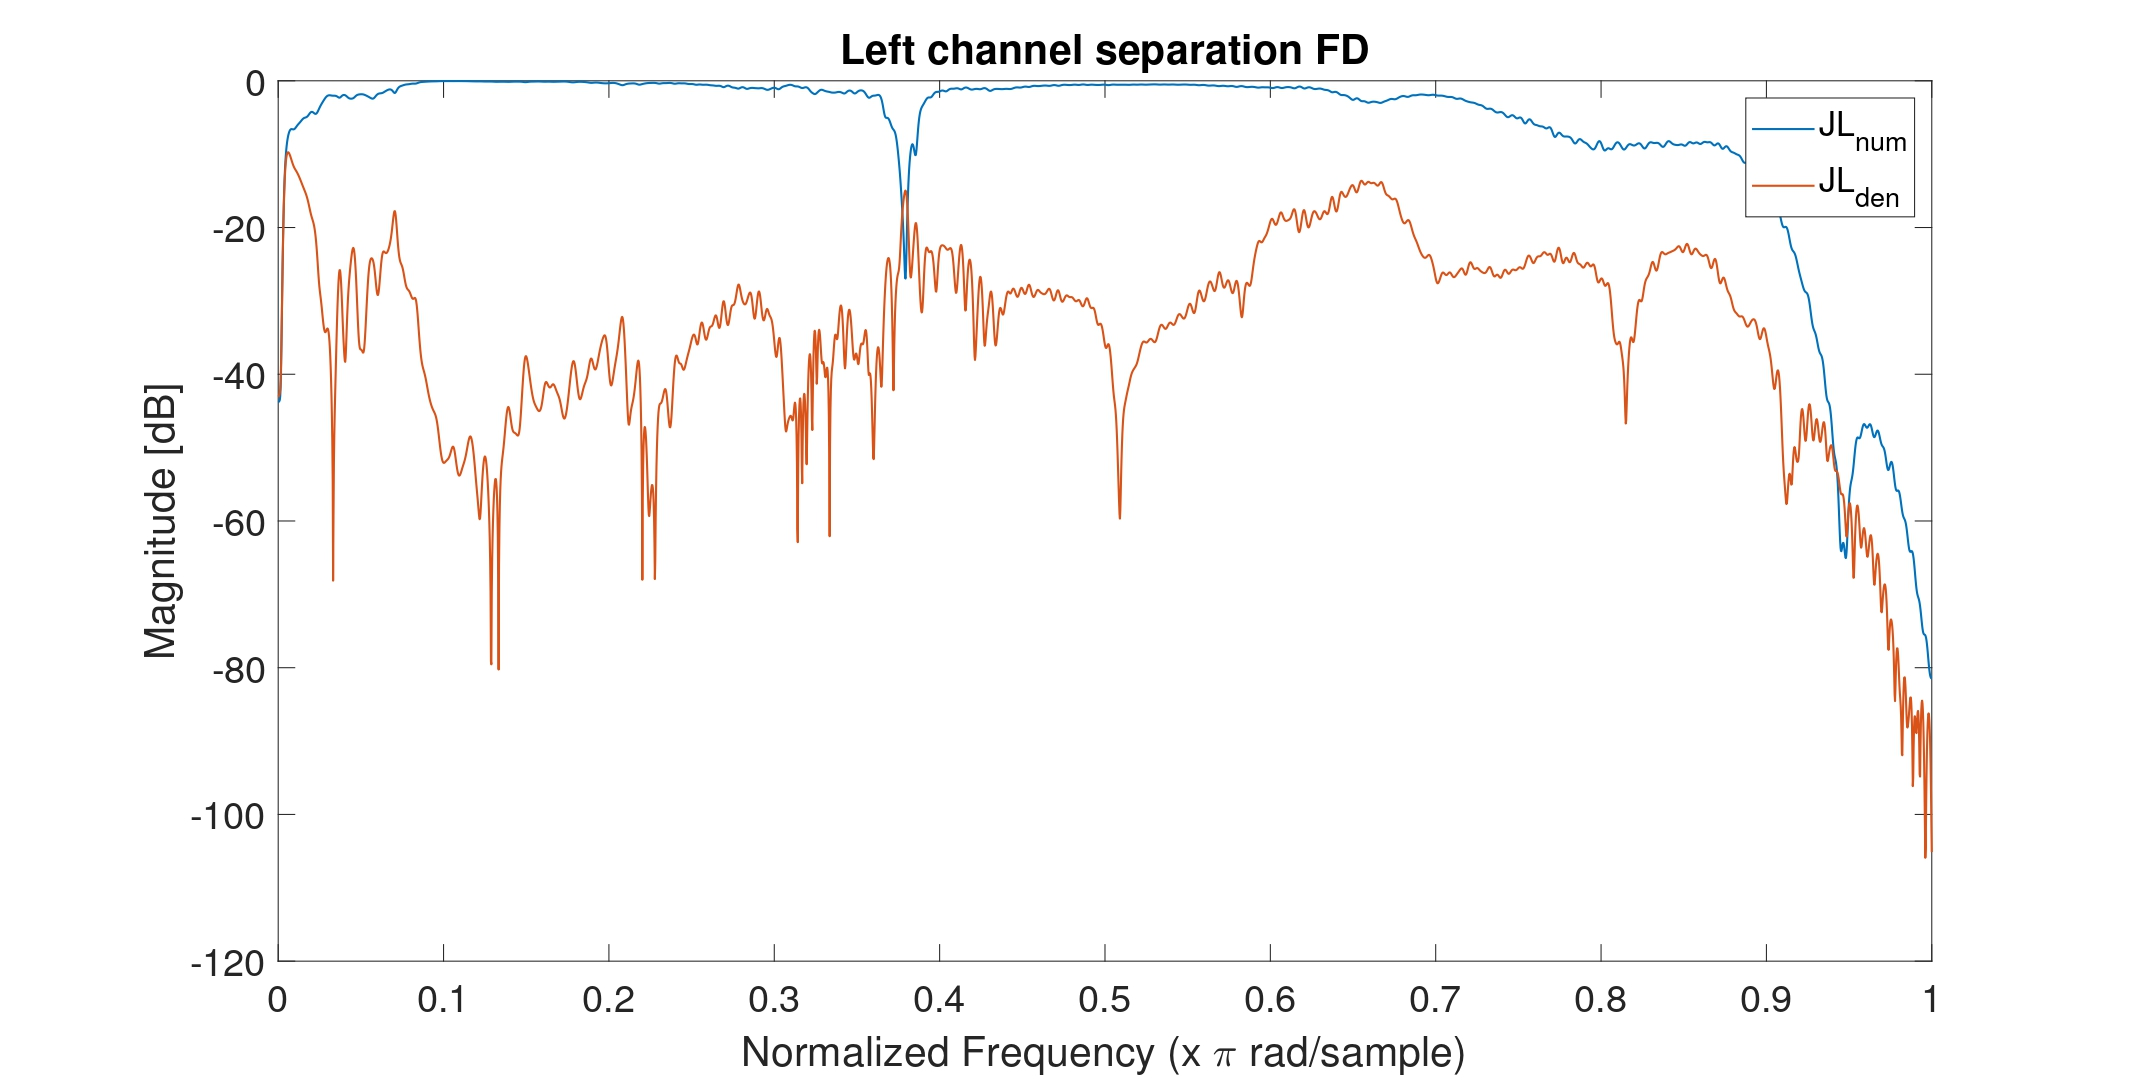
\includegraphics[width=.9\textwidth]{Immagini/left_channel_separation_FD}
	\caption{}
	\label{left_channel_separation_FD}
\end{subfigure}\\
\begin{subfigure}{1\textwidth}
	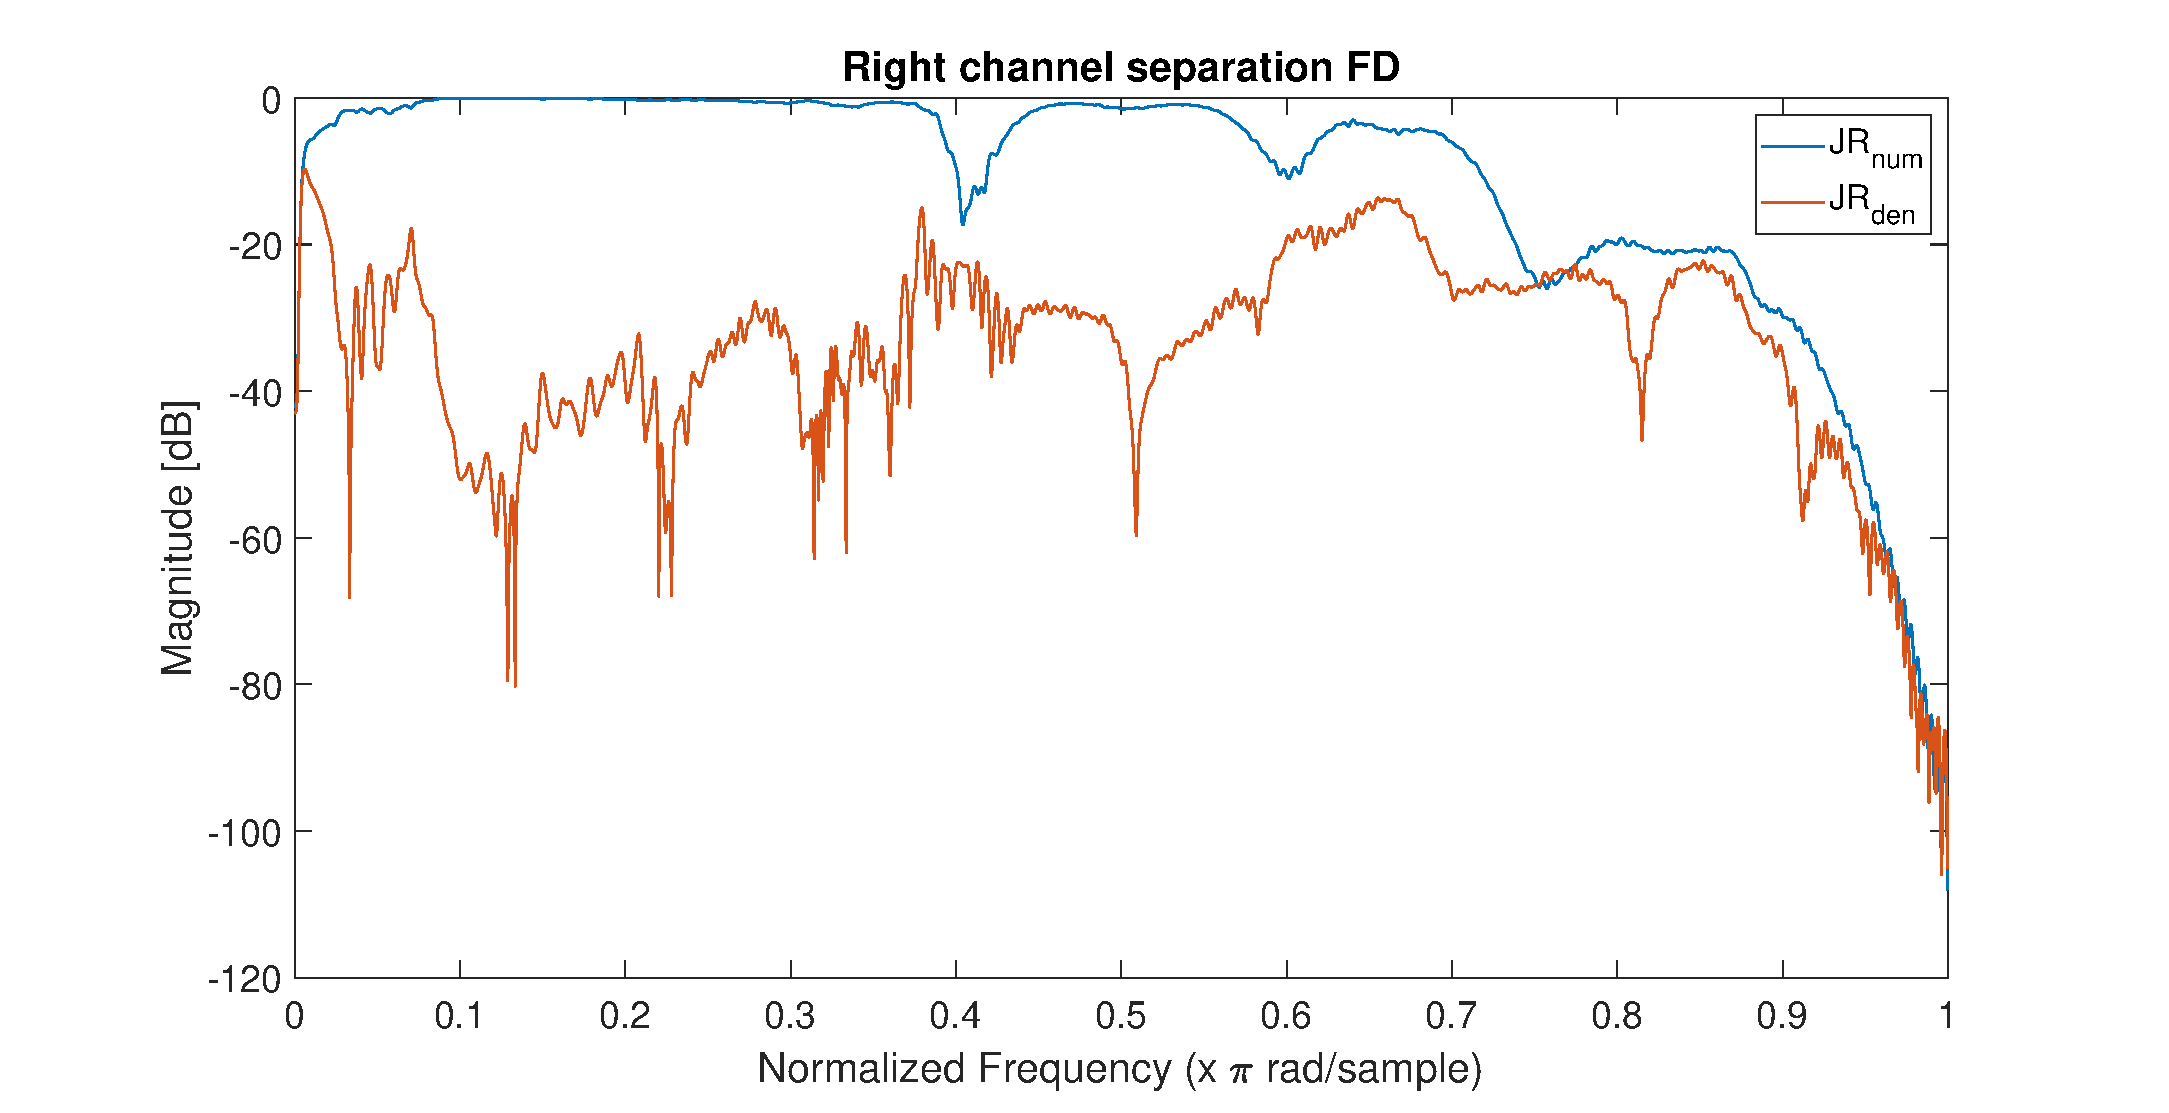
\includegraphics[width=.9\textwidth]{Immagini/right_channel_separation_FD}
	\caption{}
	\label{right_channel_separation_FD}
\end{subfigure}
\end{figure}

\begin{figure}[h]
	\ContinuedFloat
	\centering	
	\begin{subfigure}{1\textwidth}
		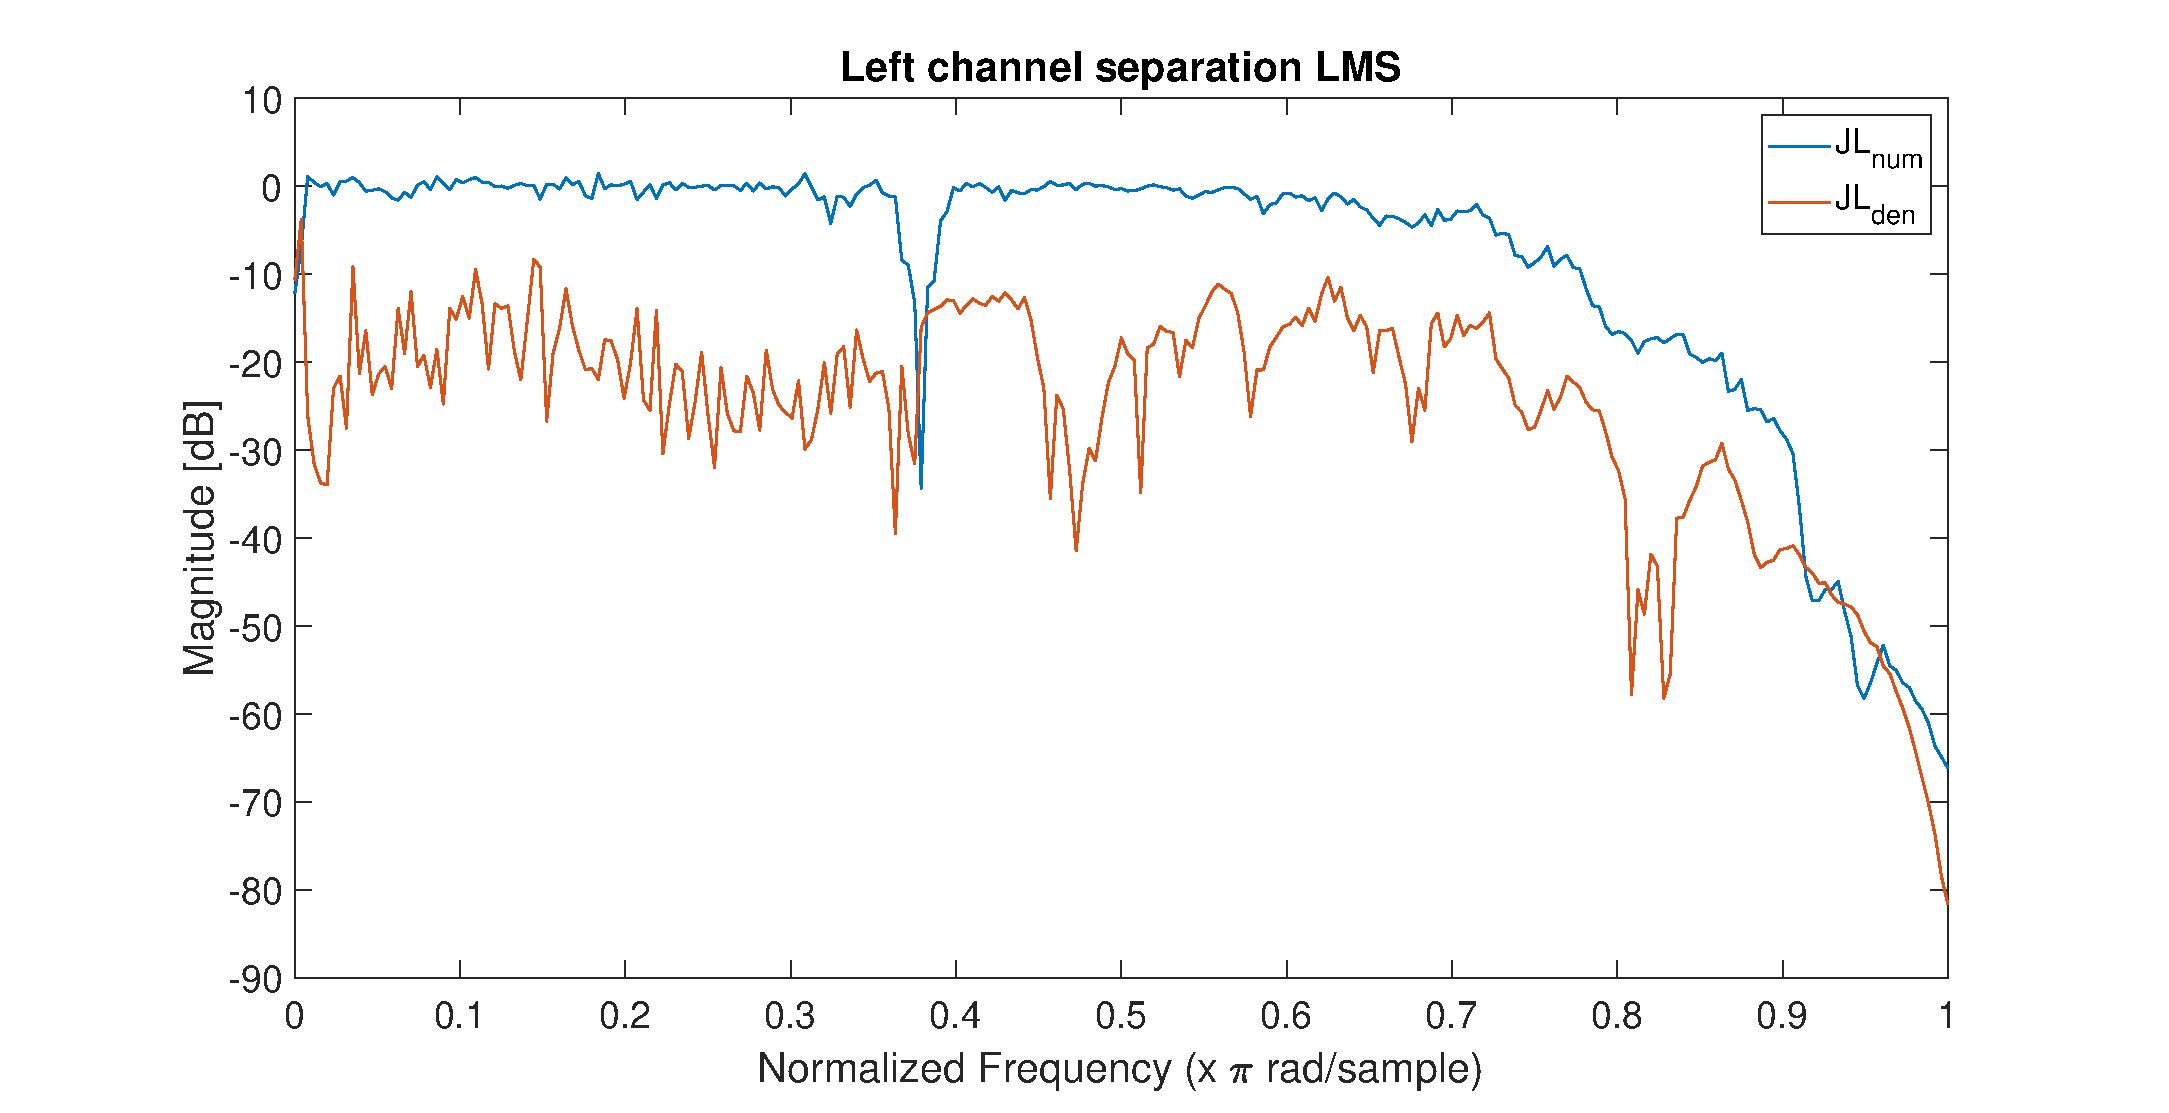
\includegraphics[width=1\textwidth]{Immagini/left_channel_separation_LMS}
		\caption{}
		\label{left_channel_separation_LMS}
	\end{subfigure}\\
	\begin{subfigure}{1\textwidth}
		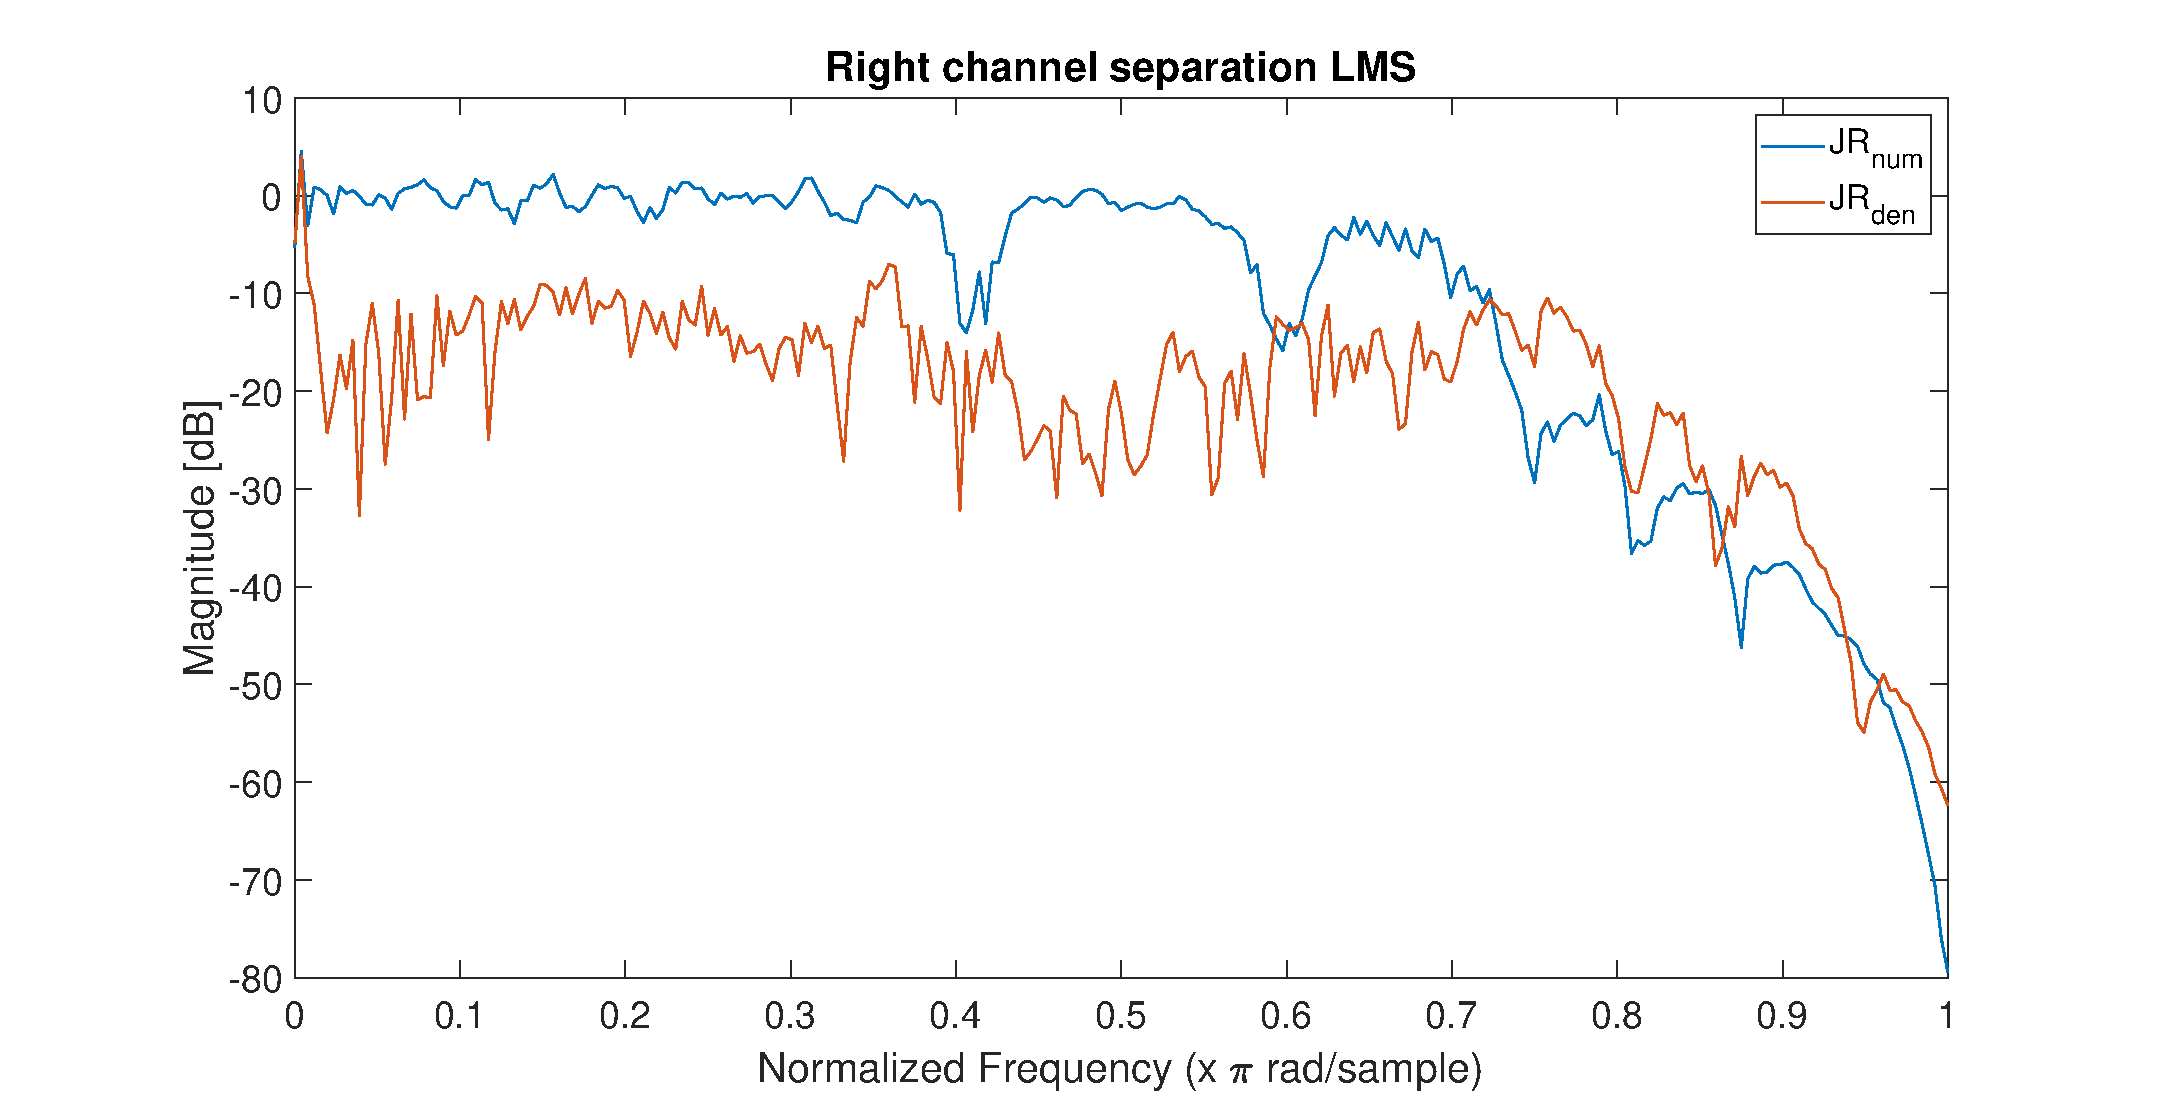
\includegraphics[width=1\textwidth]{Immagini/right_channel_separation_LMS}
		\caption{}
		\label{right_channel_separation_LMS}
	\end{subfigure}
	\caption{Confronto del numeratore e del denominatore di (a) $J_L$ e (b) $J_R$ per FD con $\beta = 0.3$, (c) $J_L$ e (d) $J_R$ per LMS con $\mu = 10^{-3}$.}
	\label{fig:channel_separation_LMS_FD}
\end{figure}

La figura~\ref{fig:mse_LMS} mostra l'andamento nel tempo del mean square error in \si{\decibel} dell'algoritmo LMS. Dalla formula~\eqref{eq:errore_lms} si ha che l'$n$-esimo valore dell'errore è dato dalla differenza tra l'$n$-esimo valore del segnale desiderato e dall'$n$-esimo valore dell'uscita. Si osserva dalla figura~\ref{fig:mse_LMS} che all'aumentare del tempo l'errore dell'algorimo LMS diminuisce: questo indica che l'algoritmo produrrà un'uscita sempre più vicina a quella desiderata. 

La figura~\ref{fig:confronto_H_LMS_FD} mostra un confronto tra i filtri di ricostruzione $H_{11}$, $H_{12}$, $H_{21}$ e $H_{22}$ degli algoritmi LMS e FD. Si nota che i filtri $H_{11}$ e $H_{22}$ trovati con LMS e FD sono più simili tra loro rispetto ai filtri $H_{12}$ e $H_{21}$. Un confronto tra i filtri ottenuti nel progetto, figura~\ref{fig:confronto_H_LMS_FD}, e quelli proposti nel paper, figura~\ref{fig:confronto_H_LMS_FD_paper}, mostra che per alcune frequenze non si ha una perfetta uguaglianza tra i filtri calcolati con LMS e quelli calcolati con FD.

\begin{figure}[h]
	\begin{subfigure}{1\textwidth}
		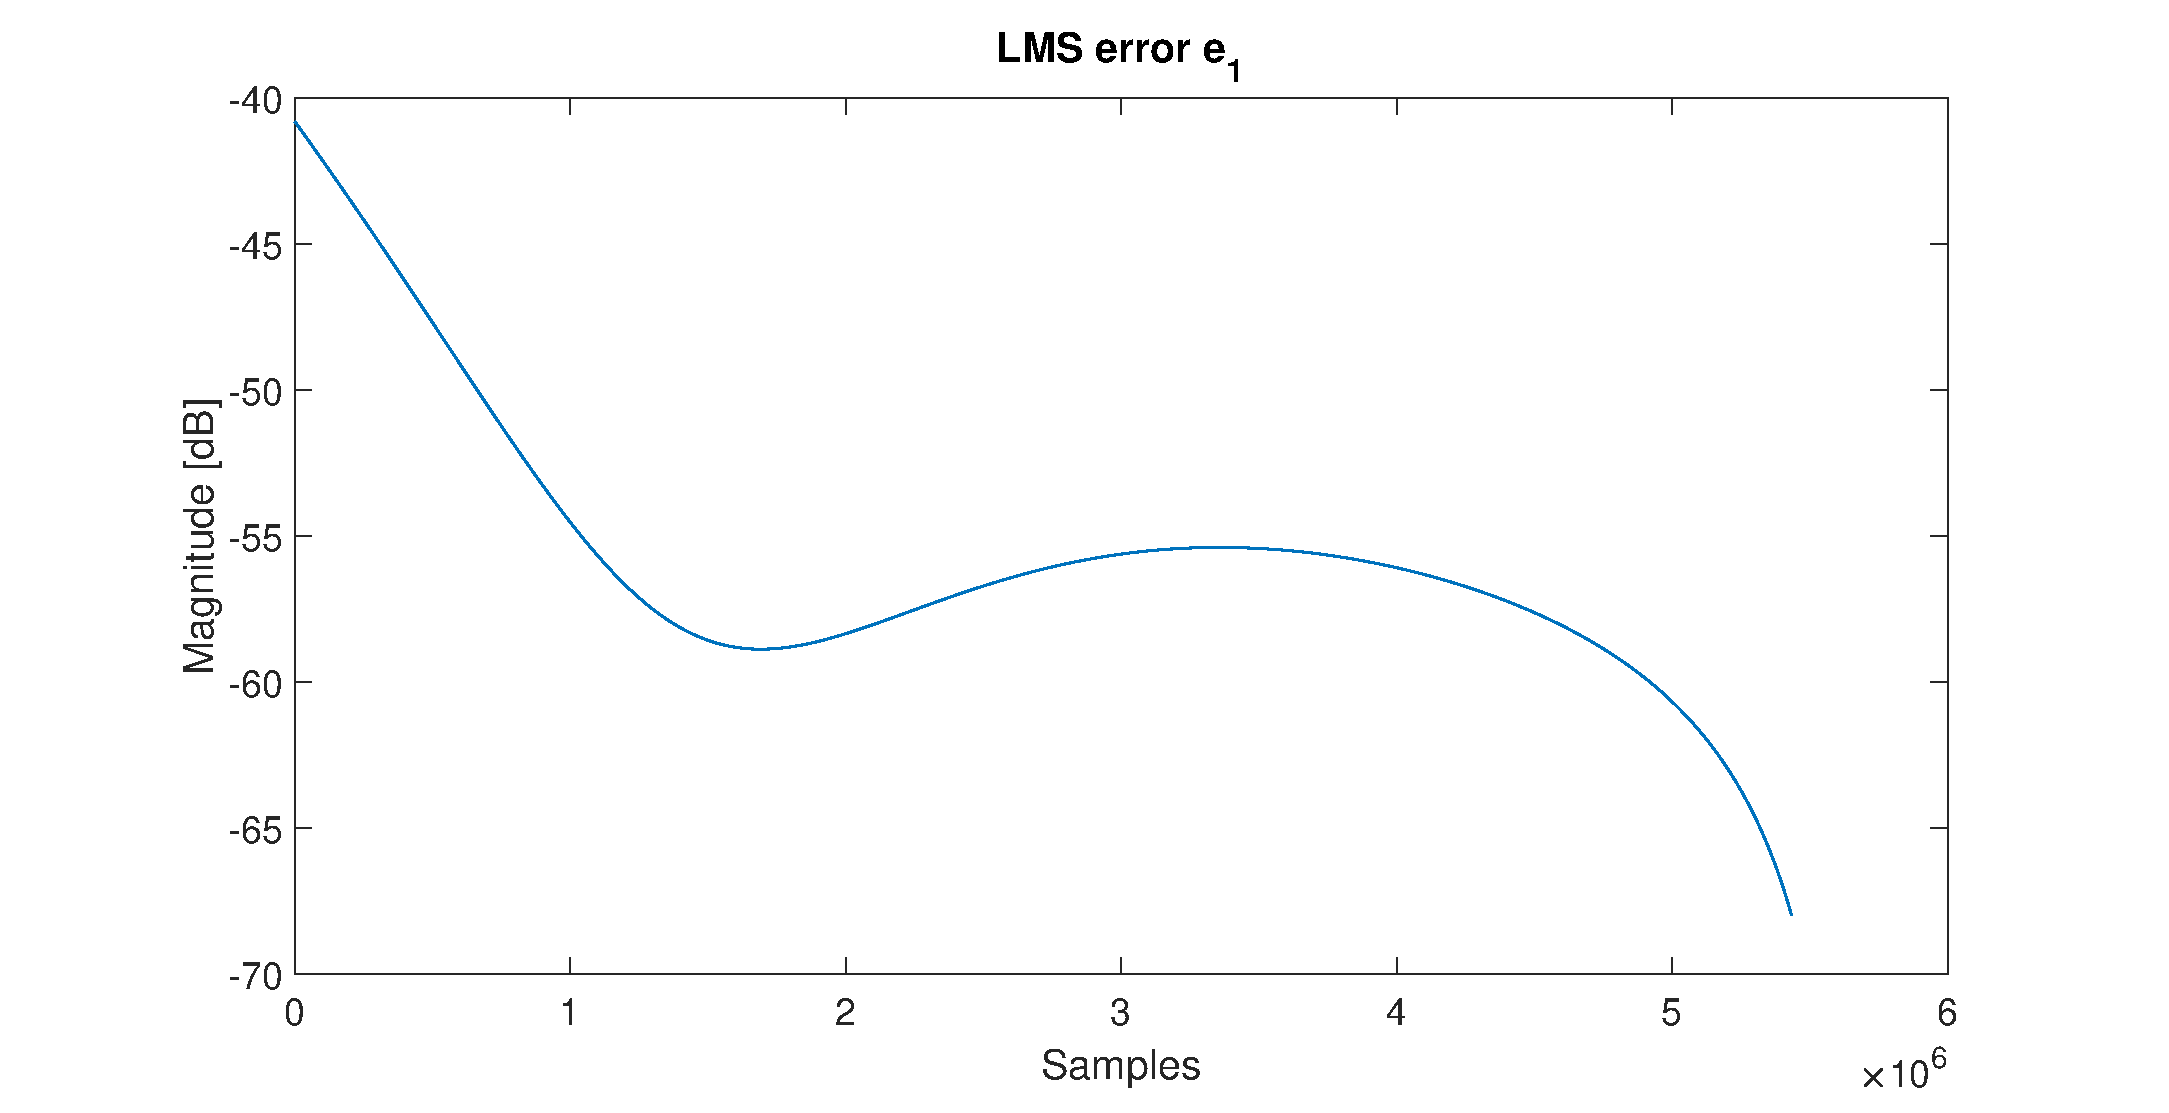
\includegraphics[width=1\textwidth]{Immagini/mse_e1}
		\caption{}
		\label{mse_e1}
	\end{subfigure}\\
	\begin{subfigure}{1\textwidth}
		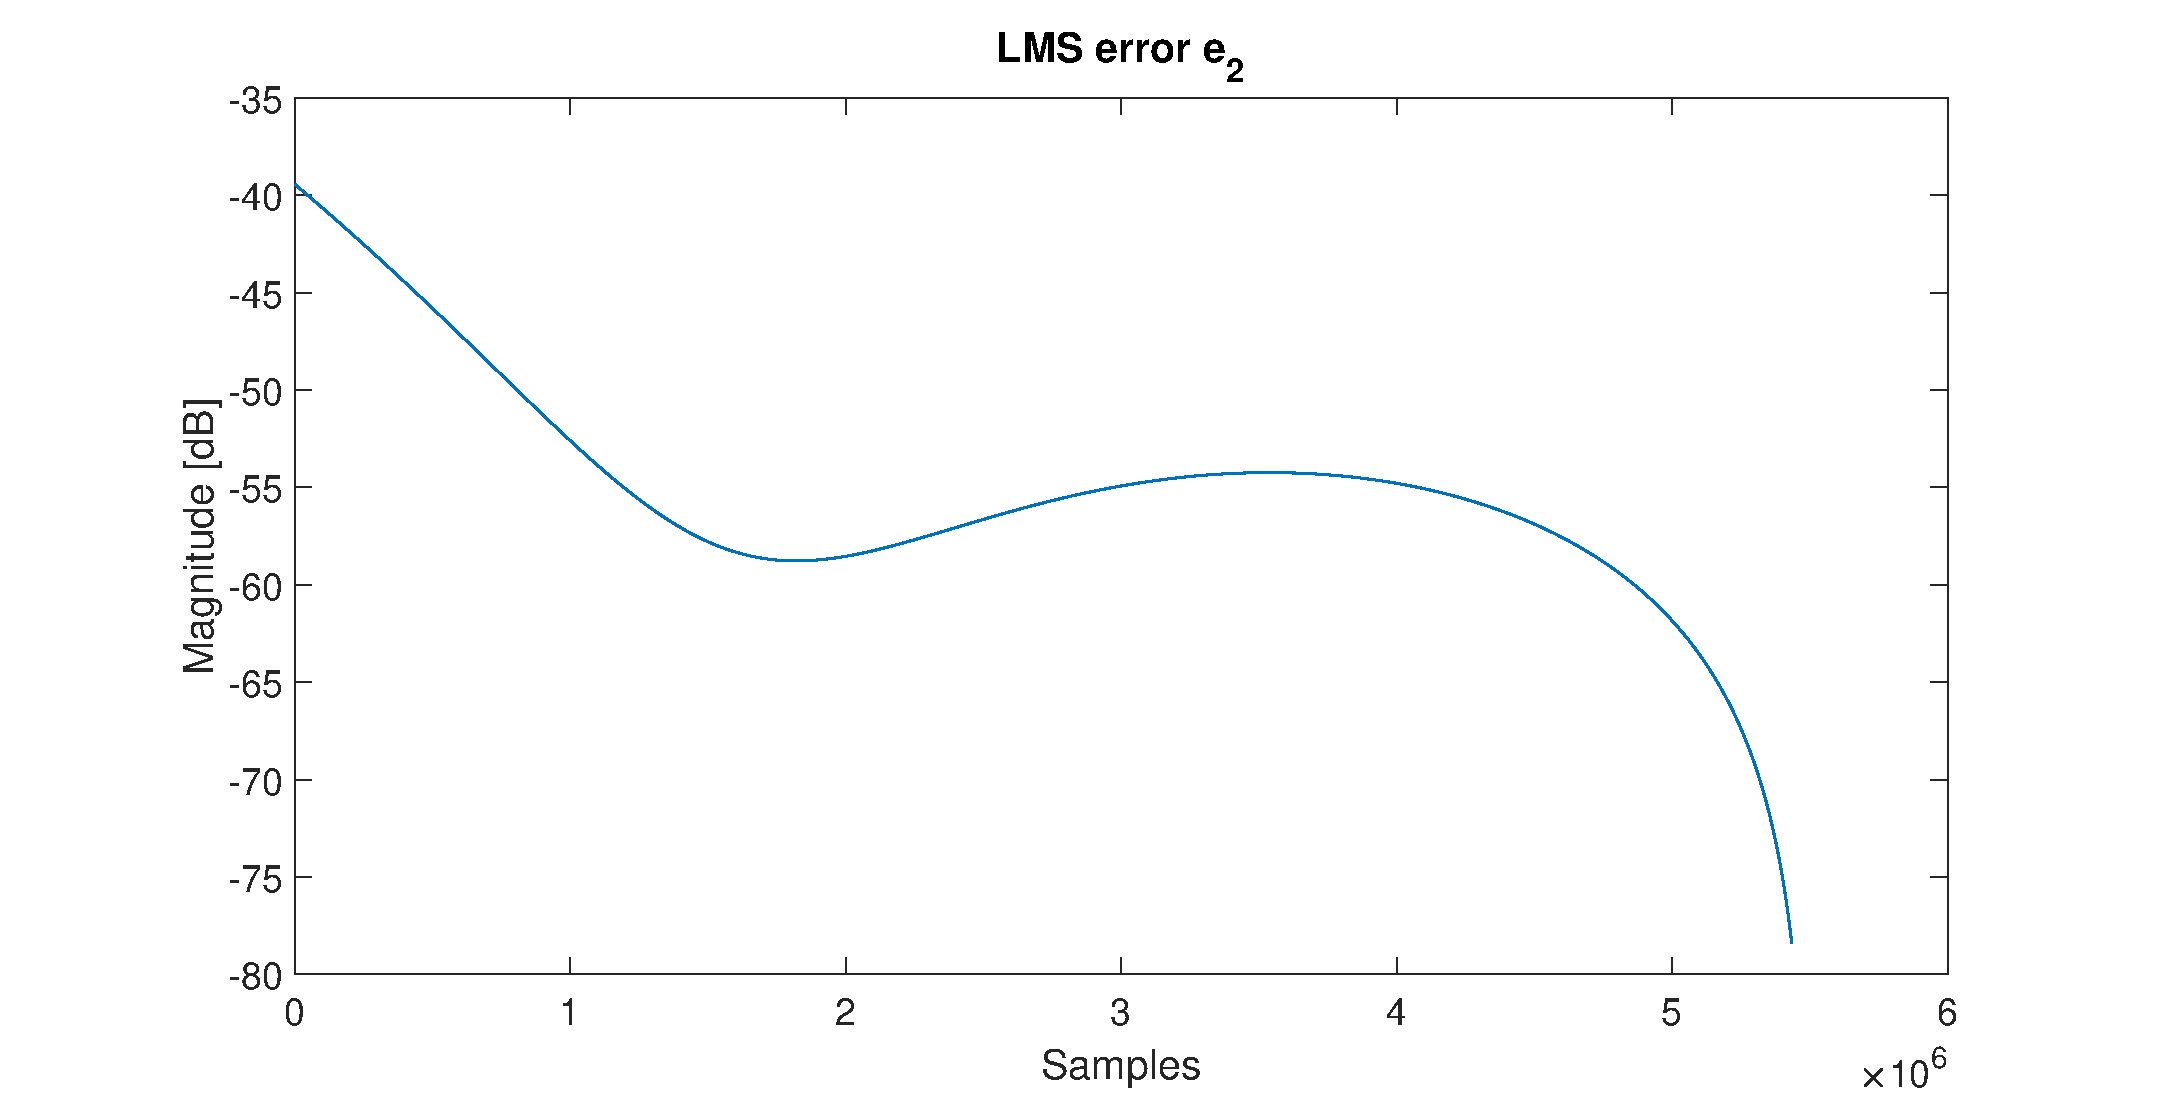
\includegraphics[width=1\textwidth]{Immagini/mse_e2}
		\caption{}
		\label{mse_e2}
	\end{subfigure}
	\caption{Confronto dell'MSE del canale (a) sinistro e (b) destro dell'algoritmo LMS.}
	\label{fig:mse_LMS}
\end{figure}

\begin{figure}[h]
	\centering
	\begin{subfigure}{1\textwidth}
		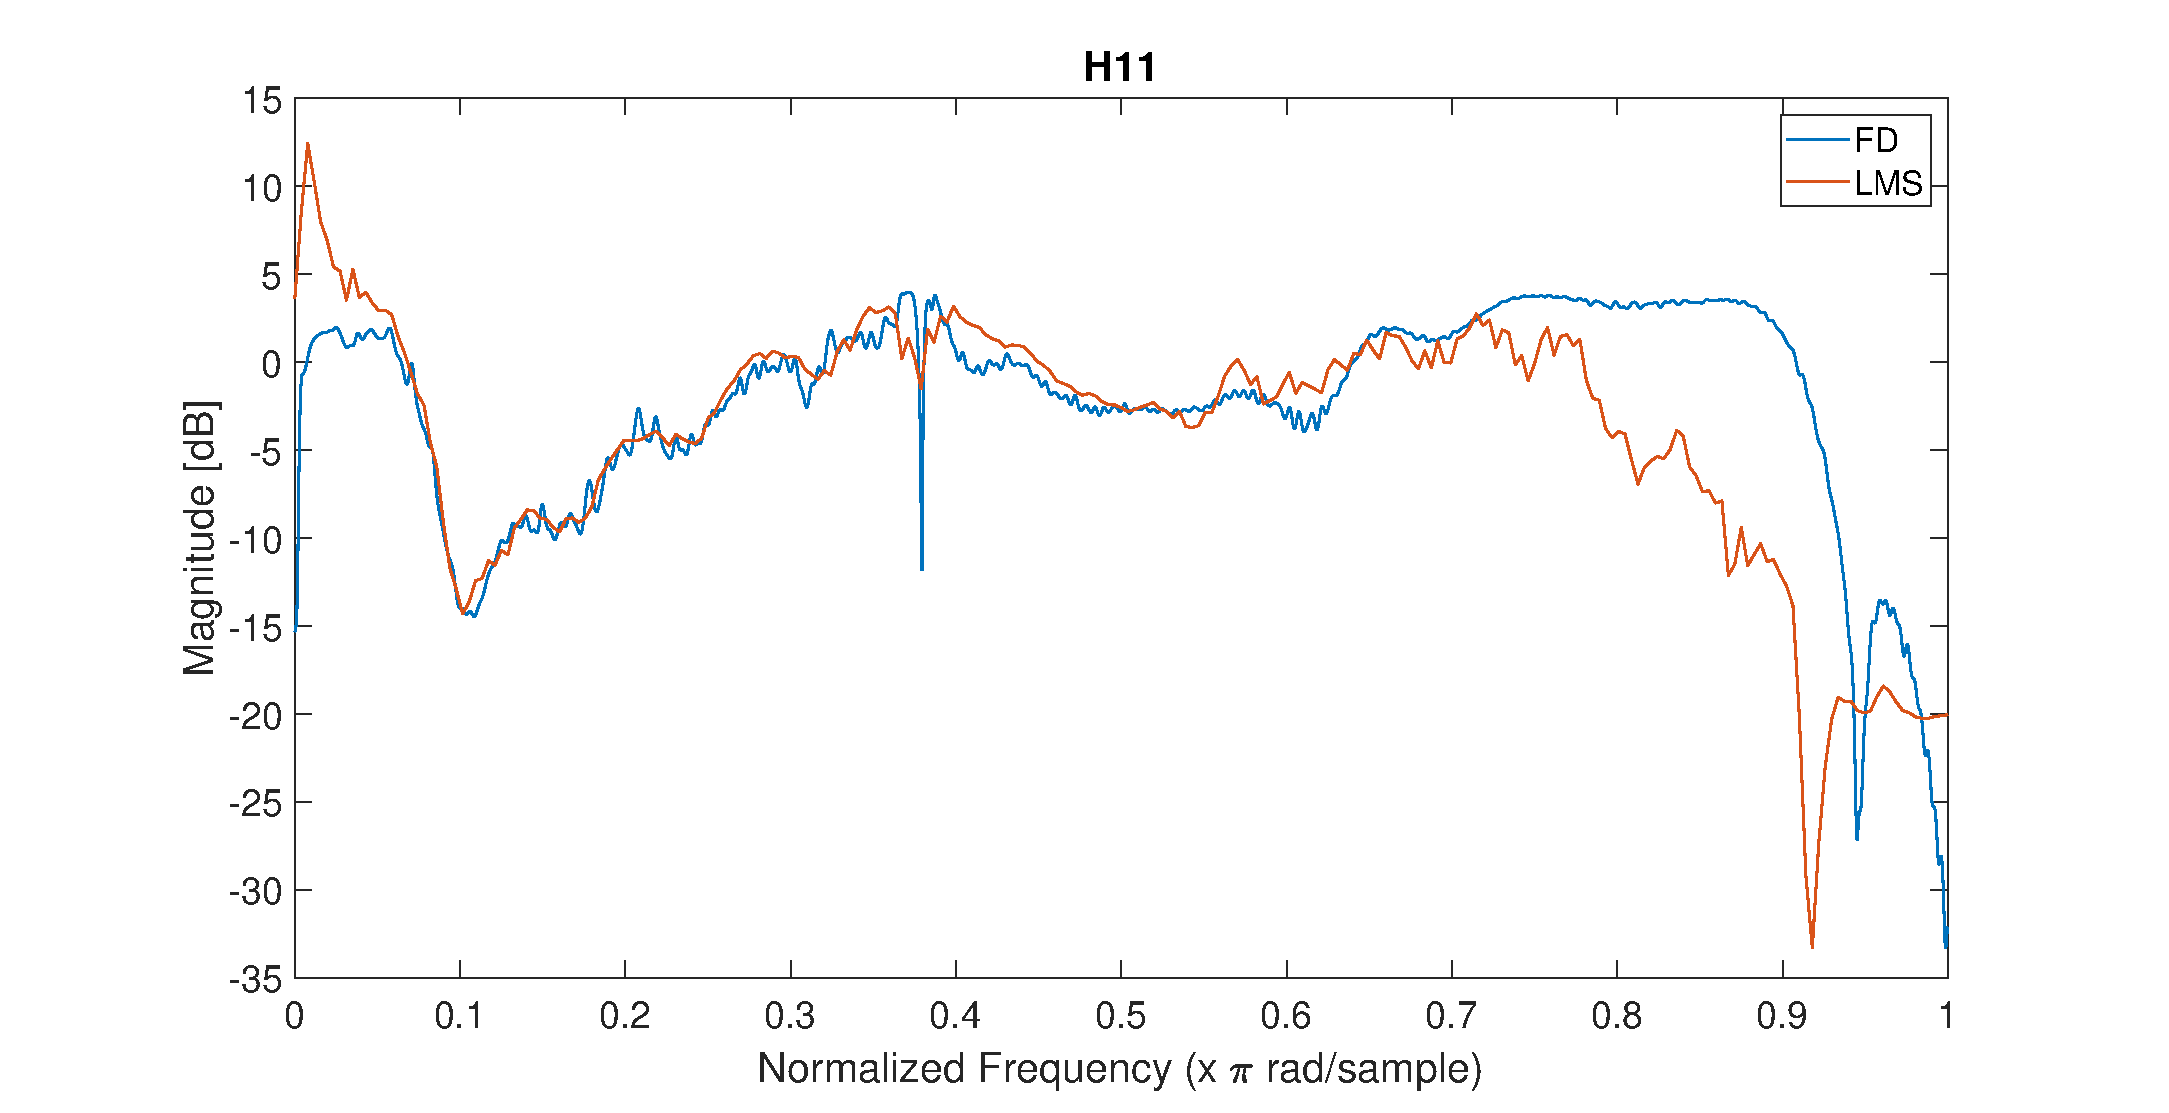
\includegraphics[width=1\textwidth]{Immagini/H11_FD_LMS}
		\caption{}
		\label{fig:Confronto_H11_LMS_FD}
	\end{subfigure}\\
	\begin{subfigure}{1\textwidth}
		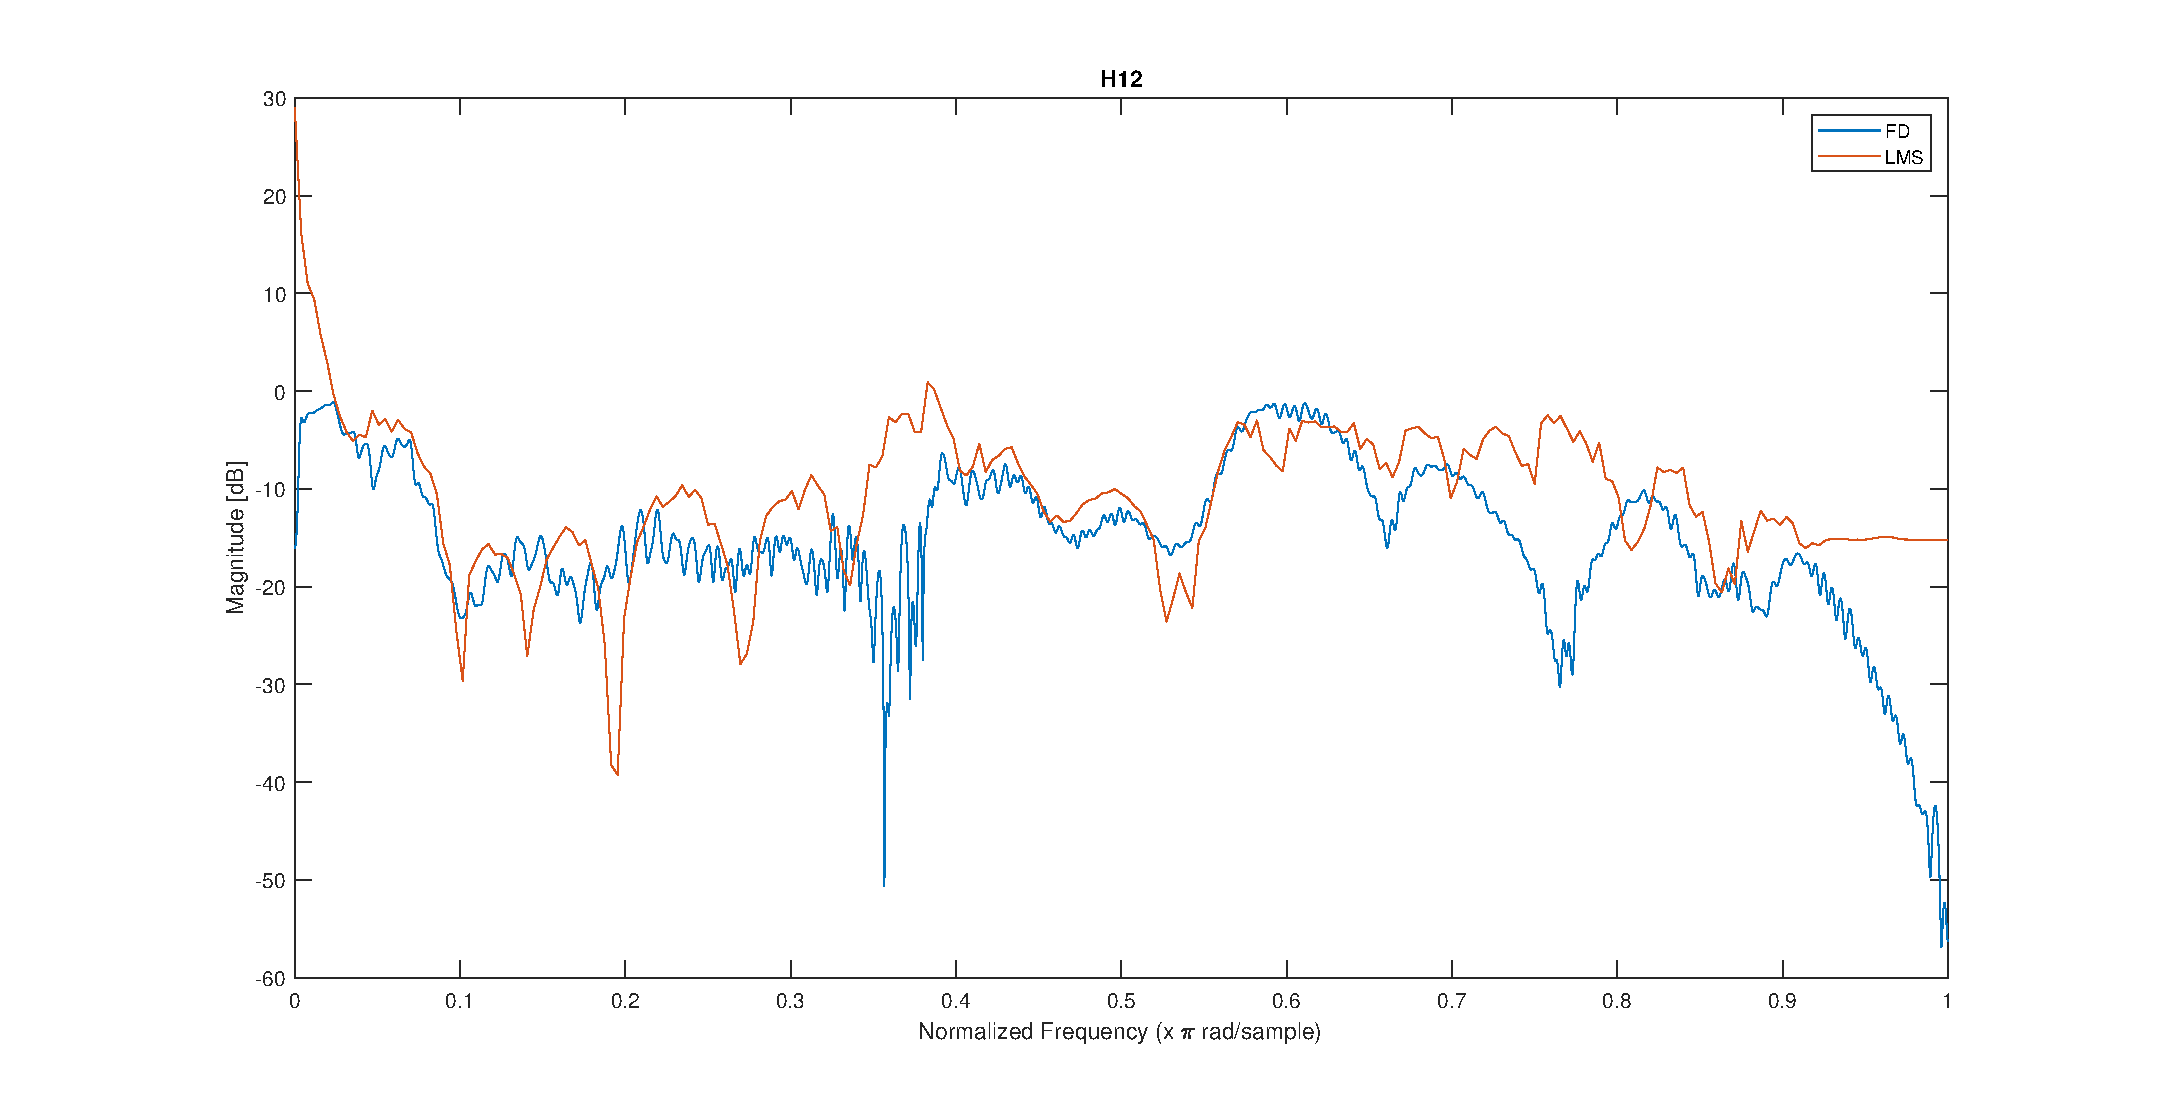
\includegraphics[width=1\textwidth]{Immagini/H12_FD_LMS}
		\caption{}
		\label{fig:Confronto_H12_LMS_FD}
	\end{subfigure}
\end{figure}

\begin{figure}[h]
	\ContinuedFloat
	\centering
	\begin{subfigure}{1\textwidth}
		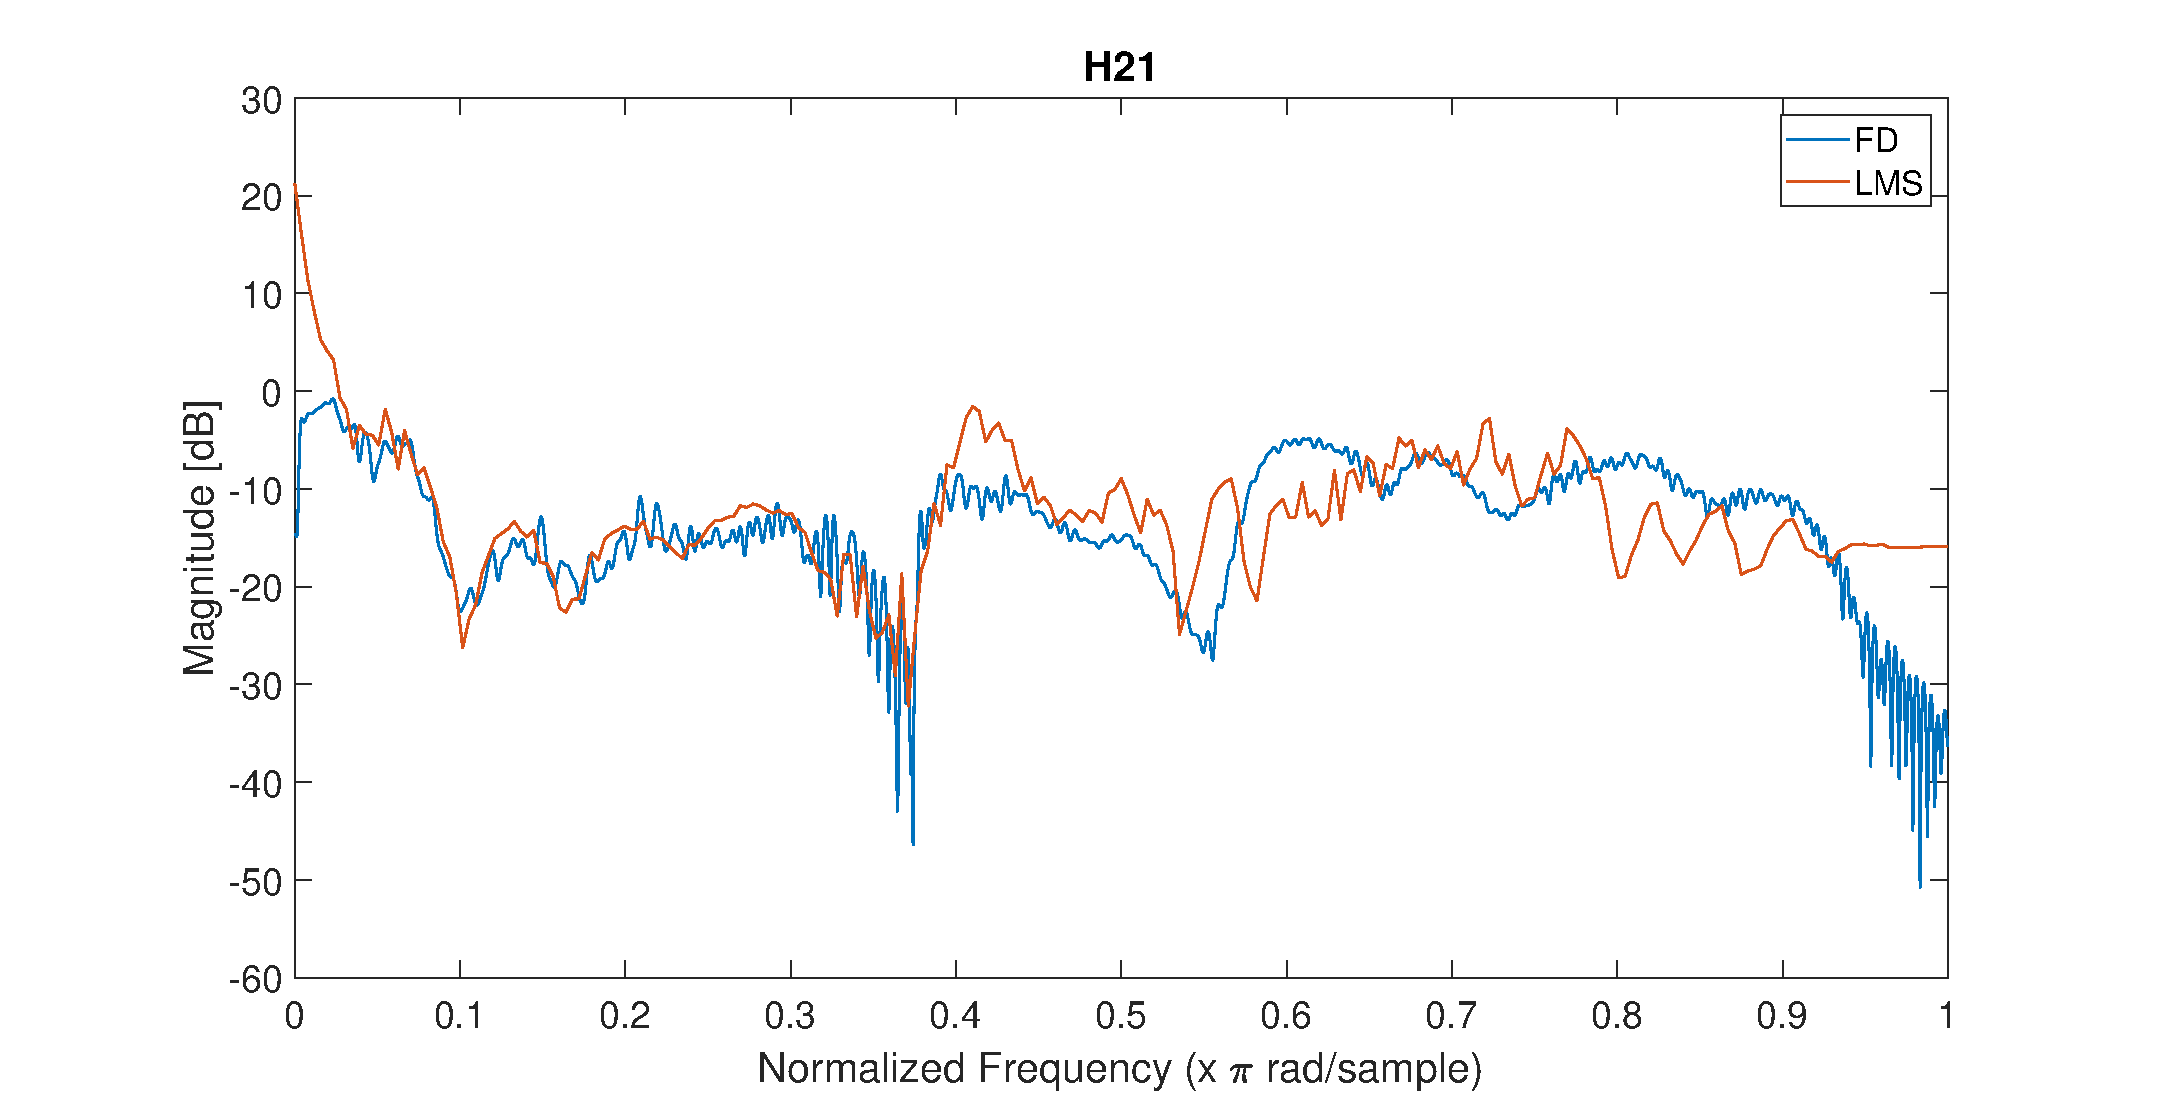
\includegraphics[width=1\textwidth]{Immagini/H21_FD_LMS}
		\caption{}
		\label{fig:Confronto_H21_LMS_FD}
	\end{subfigure}\\
	\begin{subfigure}{1\textwidth}
		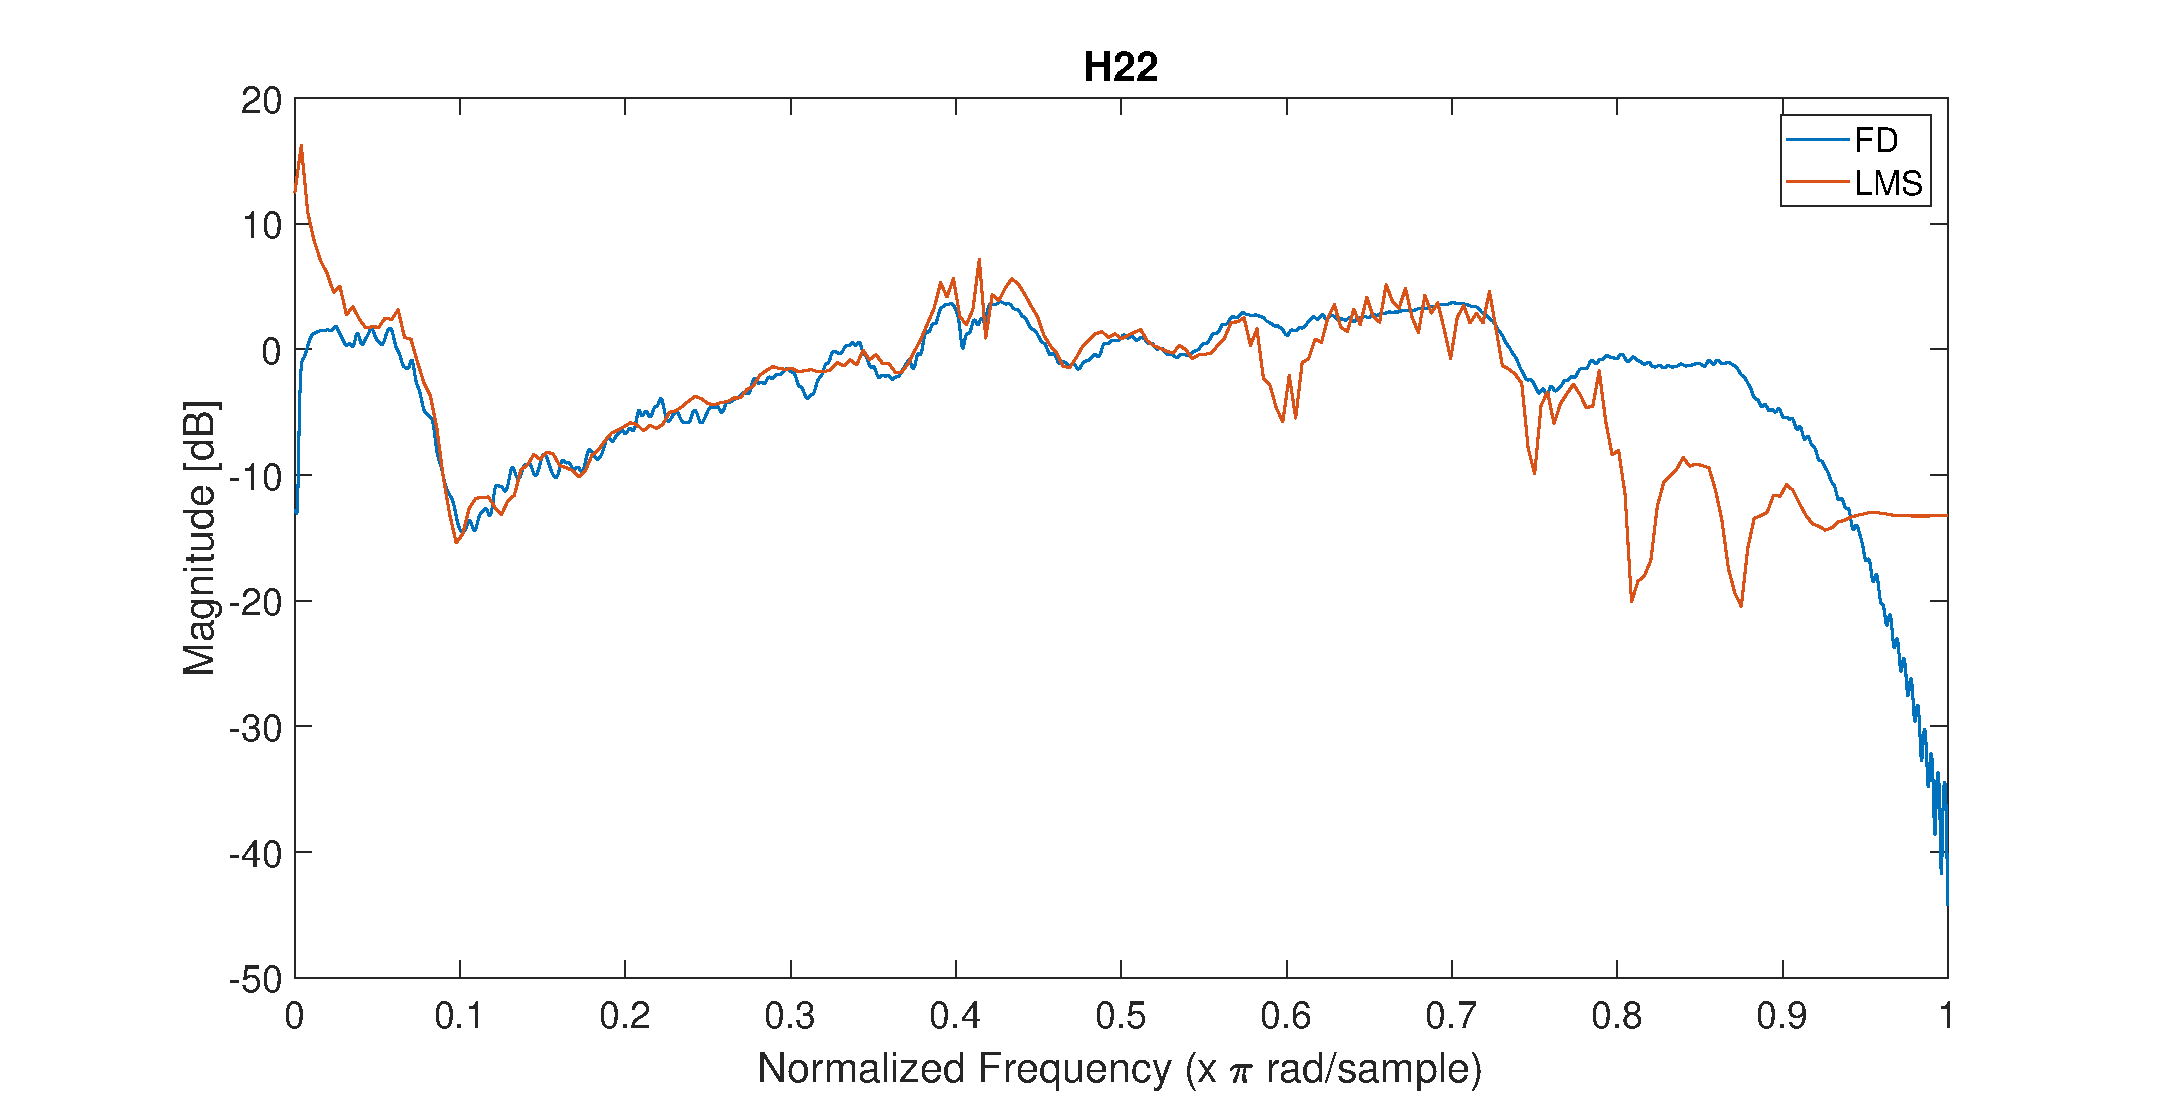
\includegraphics[width=1\textwidth]{Immagini/H22_FD_LMS}
		\caption{}
		\label{fig:Confronto_H22_LMS_FD}
	\end{subfigure}
	\caption{Confronto dei filtri di cancellazione del crosstalk (a) $H_{11}$, (b) $H_{12}$, (c) $H_{21}$, (d) $H_{22}$ di LMS e Fast Deconvolution.}
	\label{fig:confronto_H_LMS_FD}
\end{figure}

\begin{figure}[h]
	\centering	
	\begin{subfigure}{1\textwidth}
		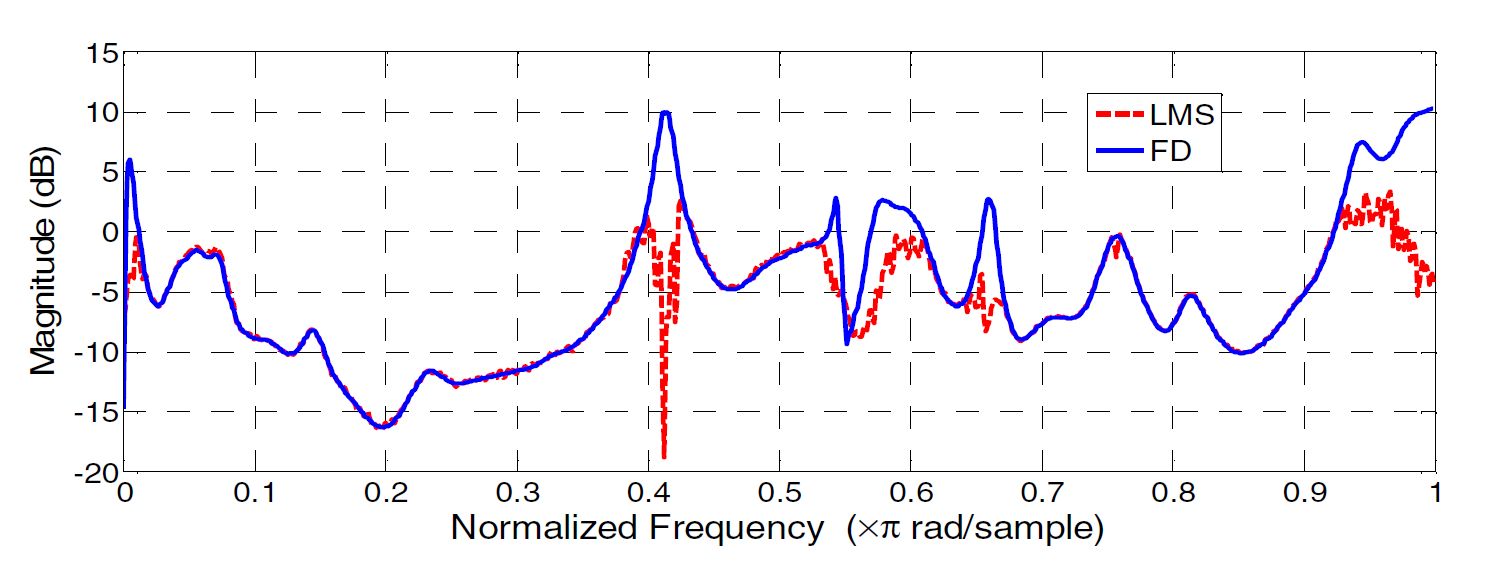
\includegraphics[width=1\textwidth]{Immagini/H11_paper}
		\caption{}
		\label{fig:Confronto_H11_LMS_FD_paper}
	\end{subfigure}\\
	\begin{subfigure}{1\textwidth}
		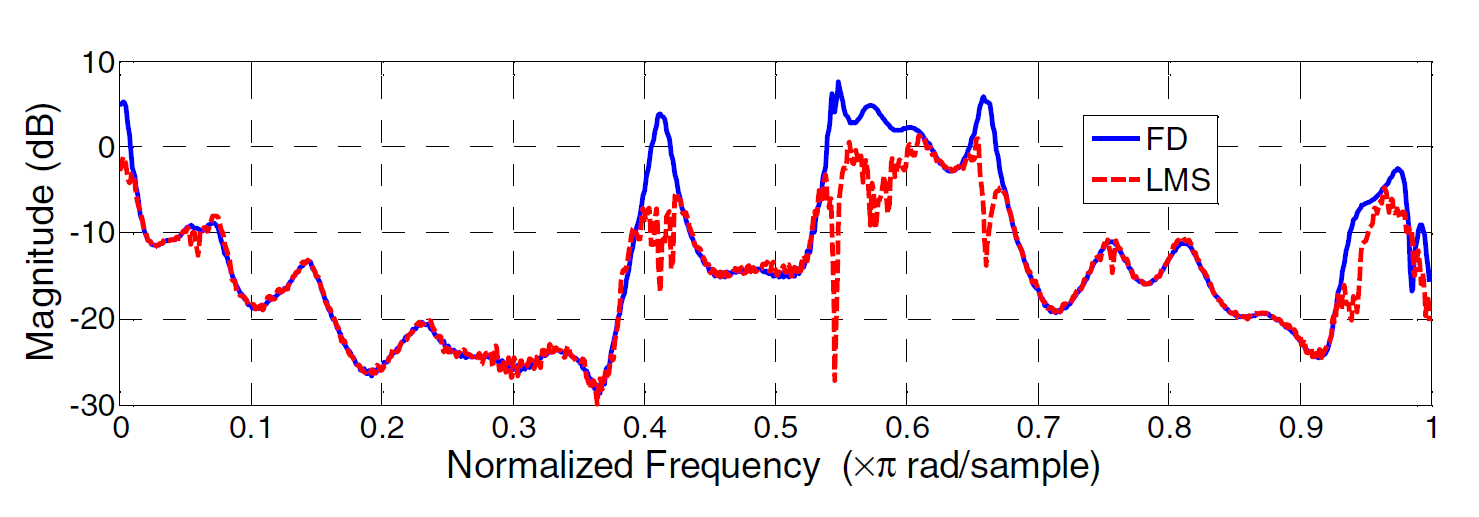
\includegraphics[width=1\textwidth]{Immagini/H12_paper}
		\caption{}
		\label{fig:Confronto_H12_LMS_FD_paper}
	\end{subfigure}	
\end{figure}
	
\begin{figure}[h]
	\ContinuedFloat
	\centering
	\begin{subfigure}{1\textwidth}
		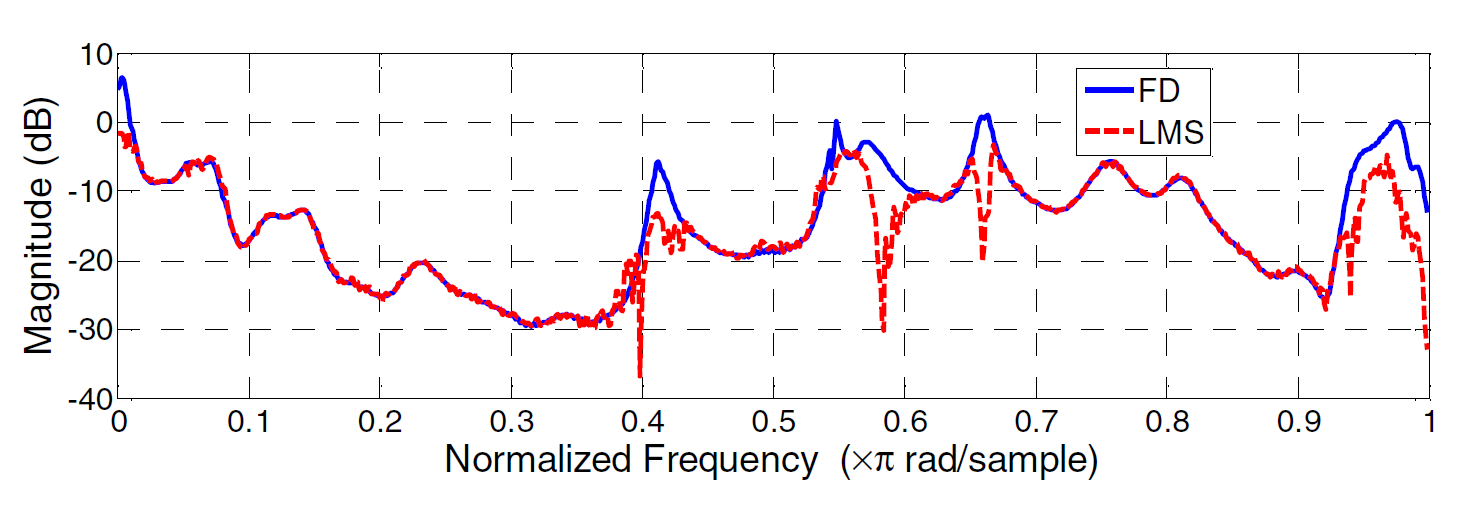
\includegraphics[width=1\textwidth]{Immagini/H21_paper}
		\caption{}
		\label{fig:Confronto_H21_LMS_FD_paper}
	\end{subfigure}\\
	\begin{subfigure}{1\textwidth}
		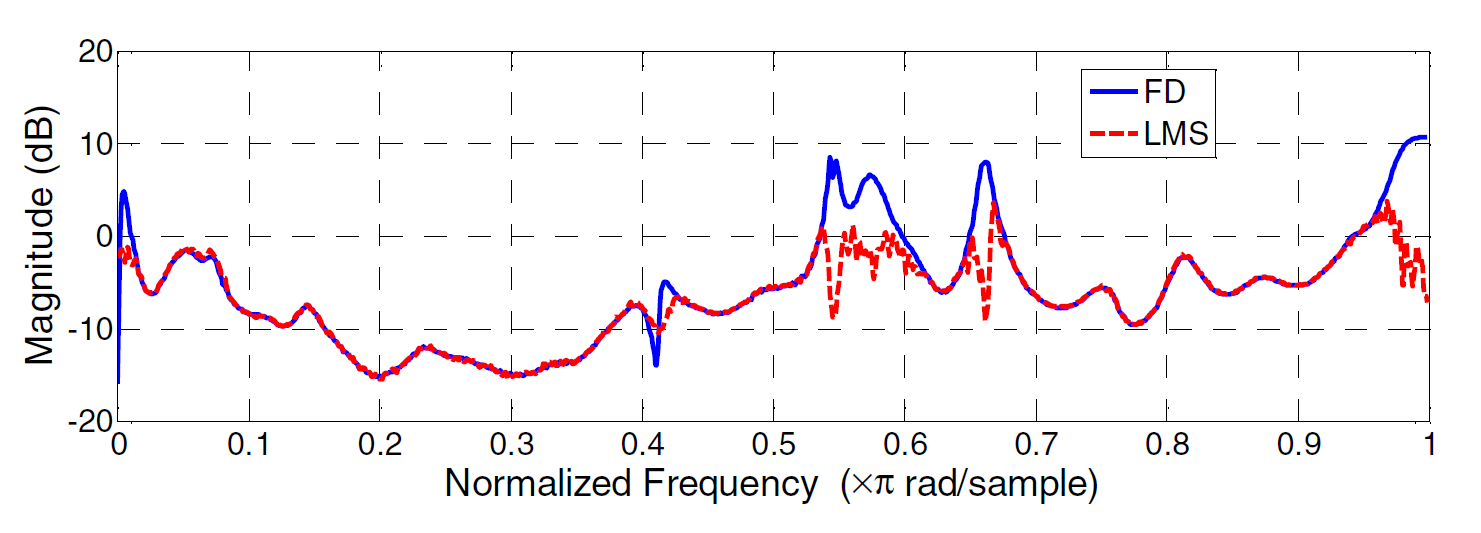
\includegraphics[width=1\textwidth]{Immagini/H22_paper}
		\caption{}
		\label{fig:Confronto_H22_LMS_FD_paper}
	\end{subfigure}
	\caption{Confronto dei filtri di cancellazione del crosstalk (a) $H_{11}$, (b) $H_{12}$, (c) $H_{21}$, (d) $H_{22}$ di LMS e Fast Deconvolution dell'articolo~\cite{Li:comprehensive_comparison}.}
	\label{fig:confronto_H_LMS_FD_paper}
\end{figure}

Le figure~\ref{fig:x1_y1_FD} e~\ref{fig:x2_y2_FD} mostrano un confronto tra gli ingressi e le uscite nell'algoritmo Fast Deconvolution, mentre le figure~\ref{fig:d1_y1_LMS} e~\ref{fig:d2_y2_LMS} confrontano il segnale desiderato con l'uscita prodotta dall'LMS.

Dal confronto tra l'uscita desiderata e l'ingresso in figura~\ref{fig:confronto_ingressi_uscite_LMS_FD} si può notare come questi segnali siano sovrapposti: possiamo sostenere dunque che la cancellazione del crosstalk avviene in modo corretto.

\begin{figure}[h]
	\centering
	\begin{subfigure}{1\textwidth}
		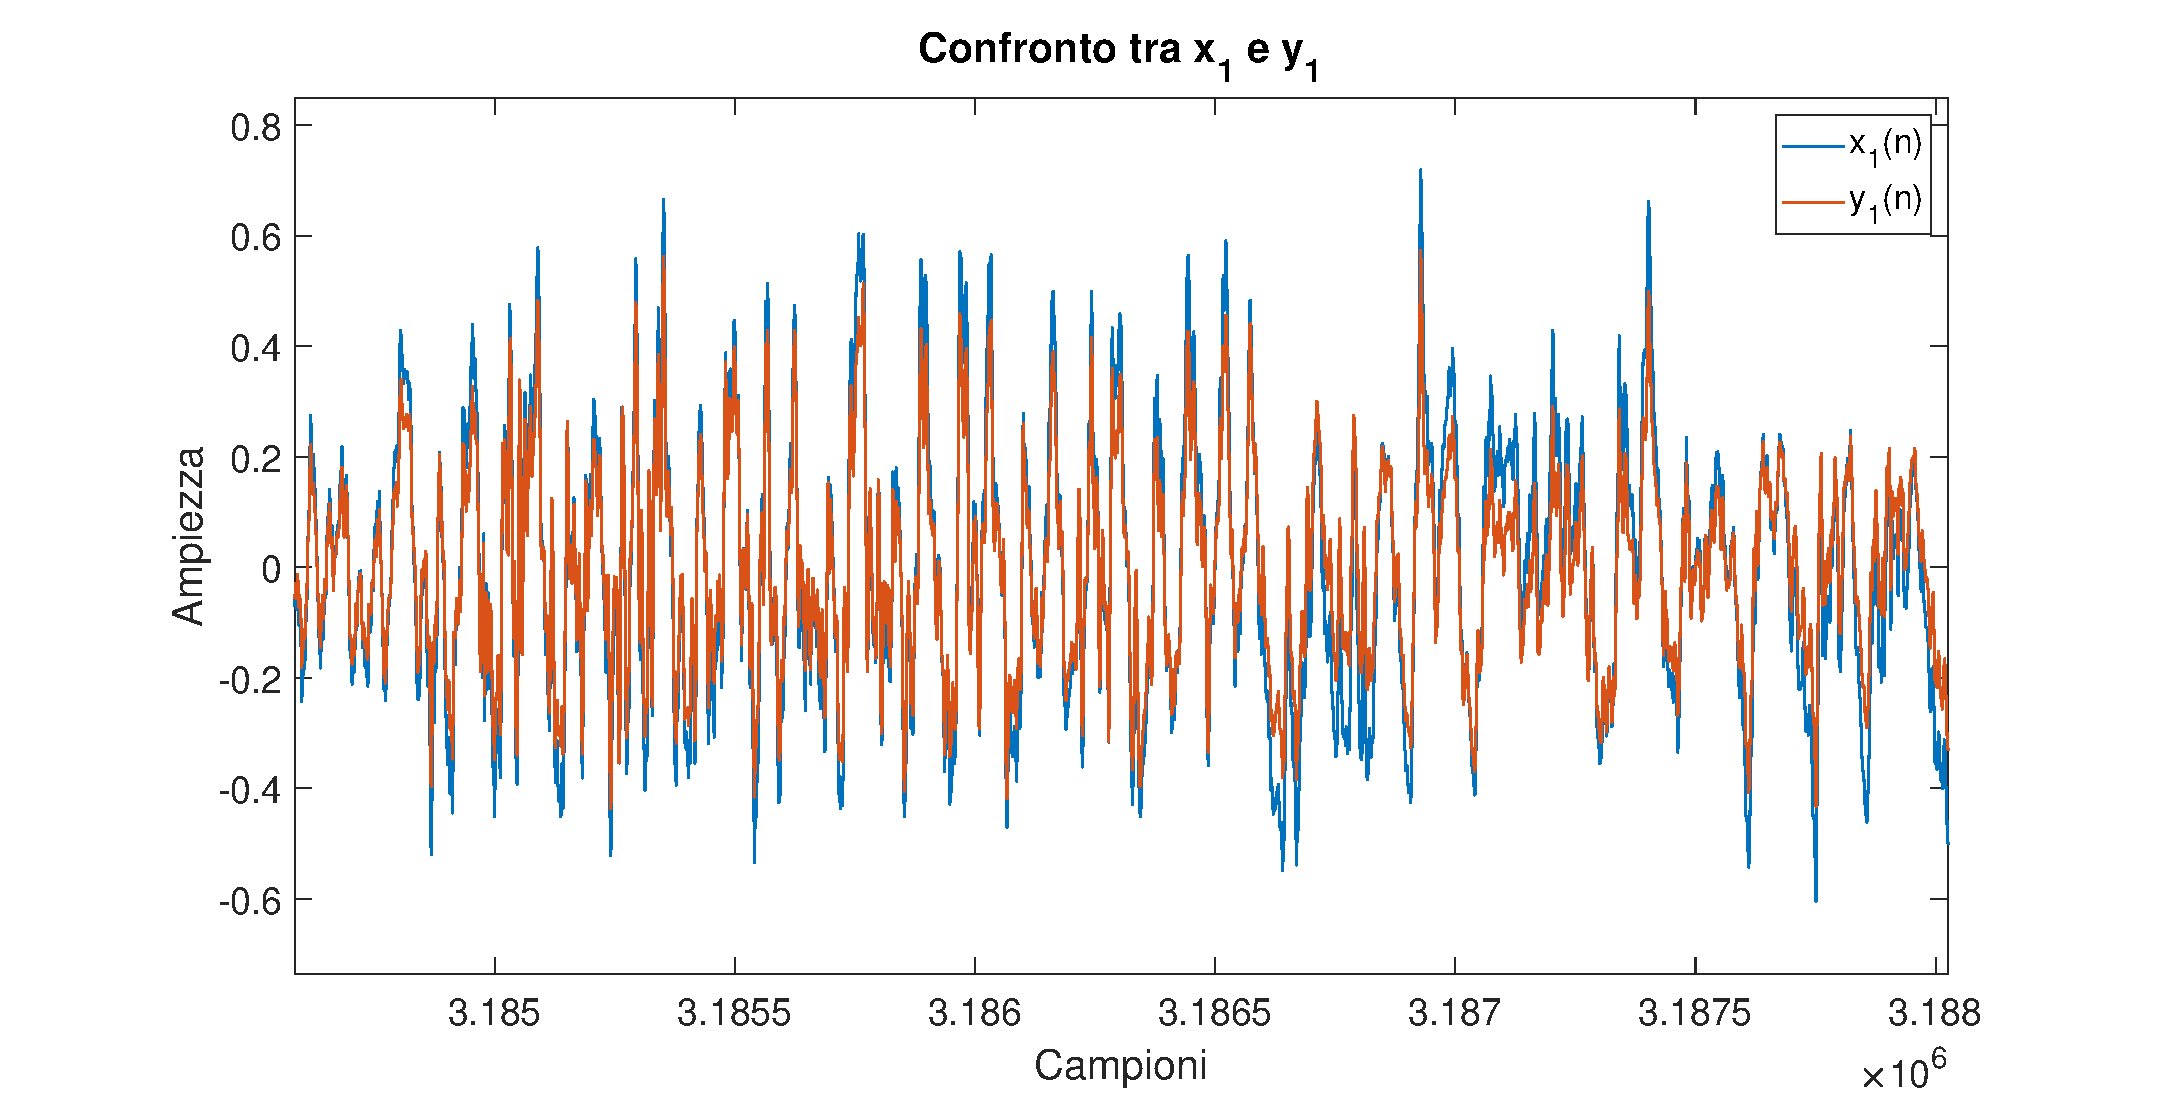
\includegraphics[width=1\textwidth]{Immagini/x1_y1_FD}
		\caption{}
		\label{fig:x1_y1_FD}
	\end{subfigure}\\
	\begin{subfigure}{1\textwidth}
		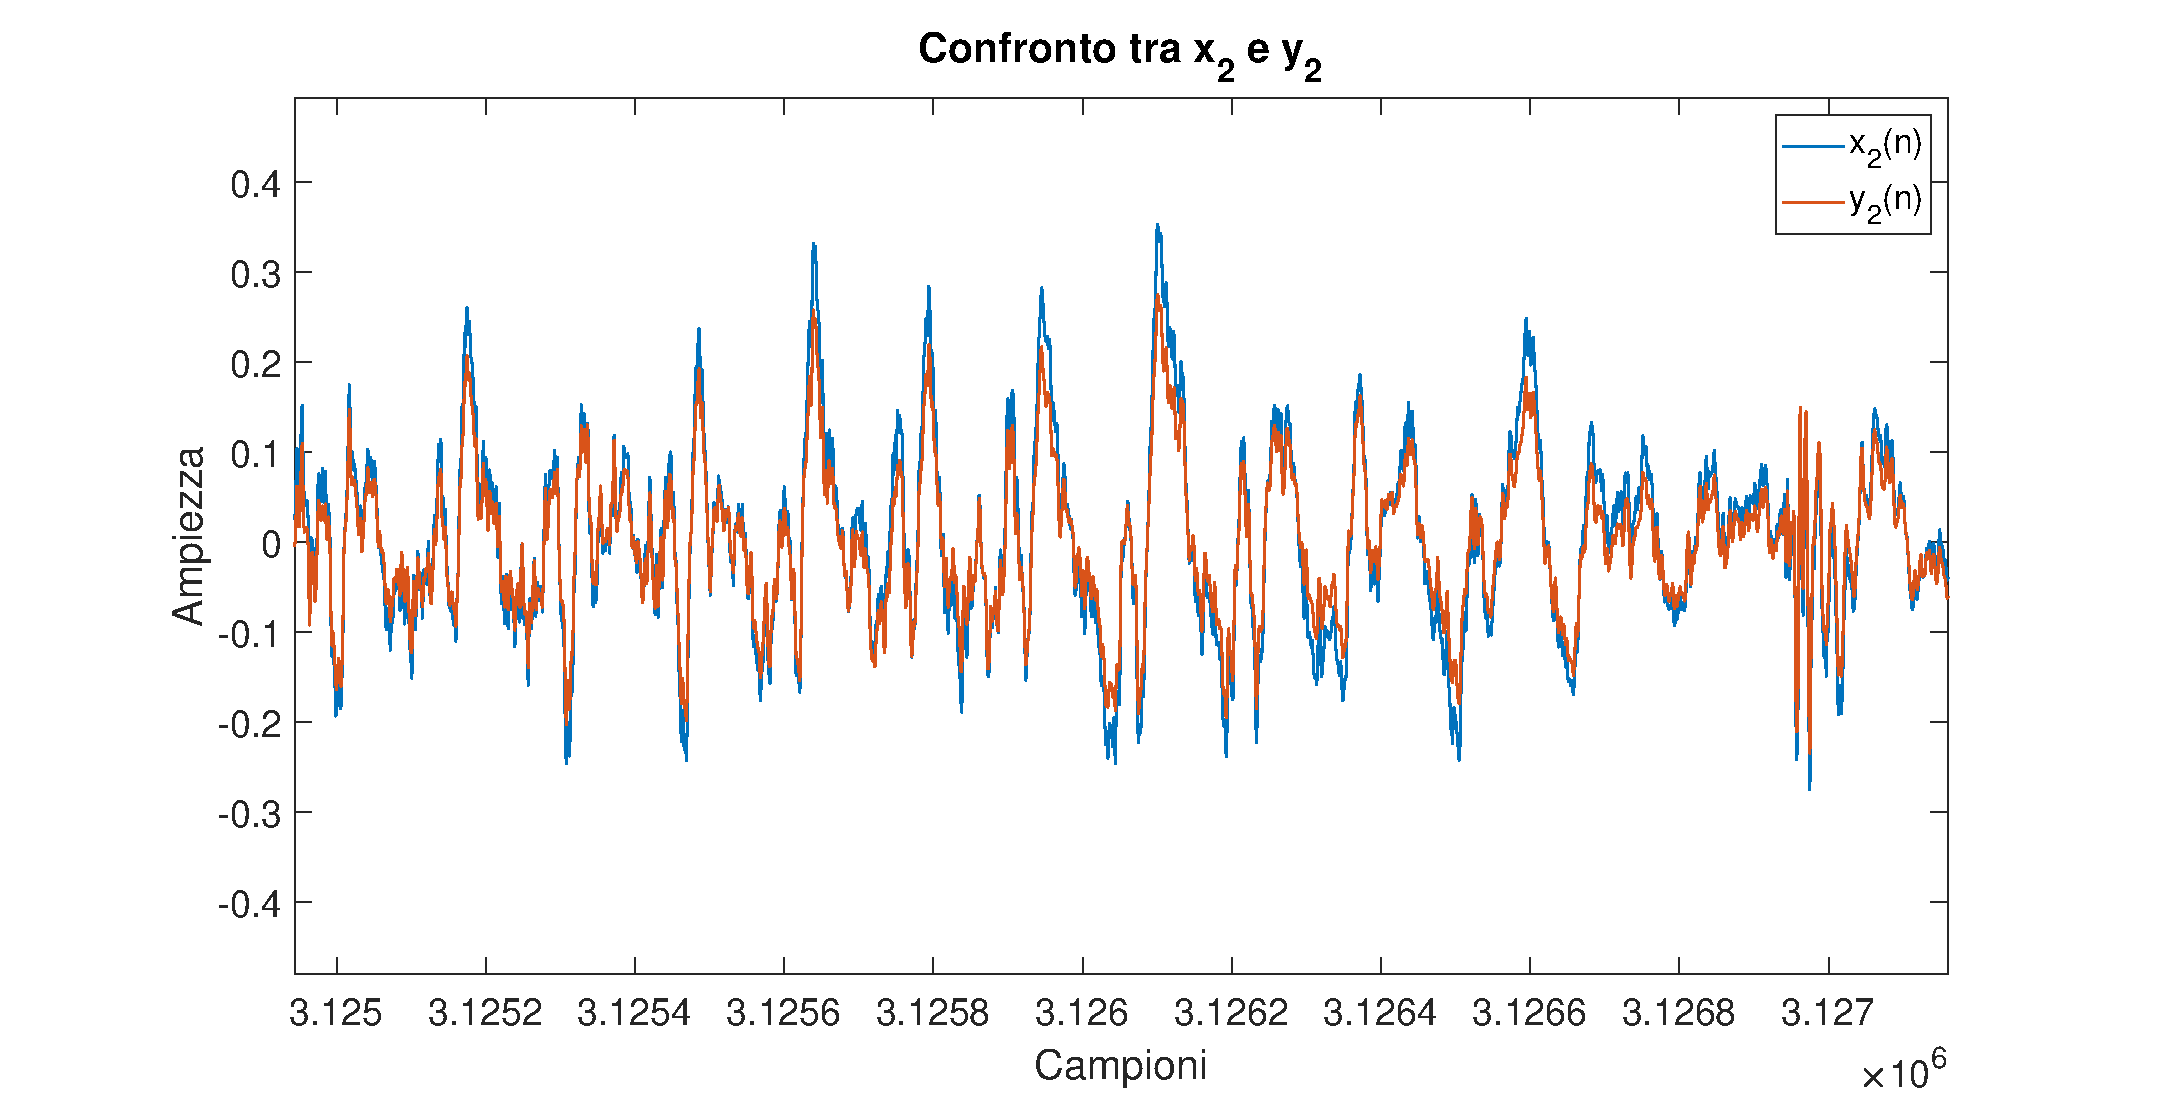
\includegraphics[width=1\textwidth]{Immagini/x2_y2_FD}
		\caption{}
		\label{fig:x2_y2_FD}
	\end{subfigure}
\end{figure}

\begin{figure}[h]
	\ContinuedFloat
	\centering
	\begin{subfigure}{1\textwidth}
		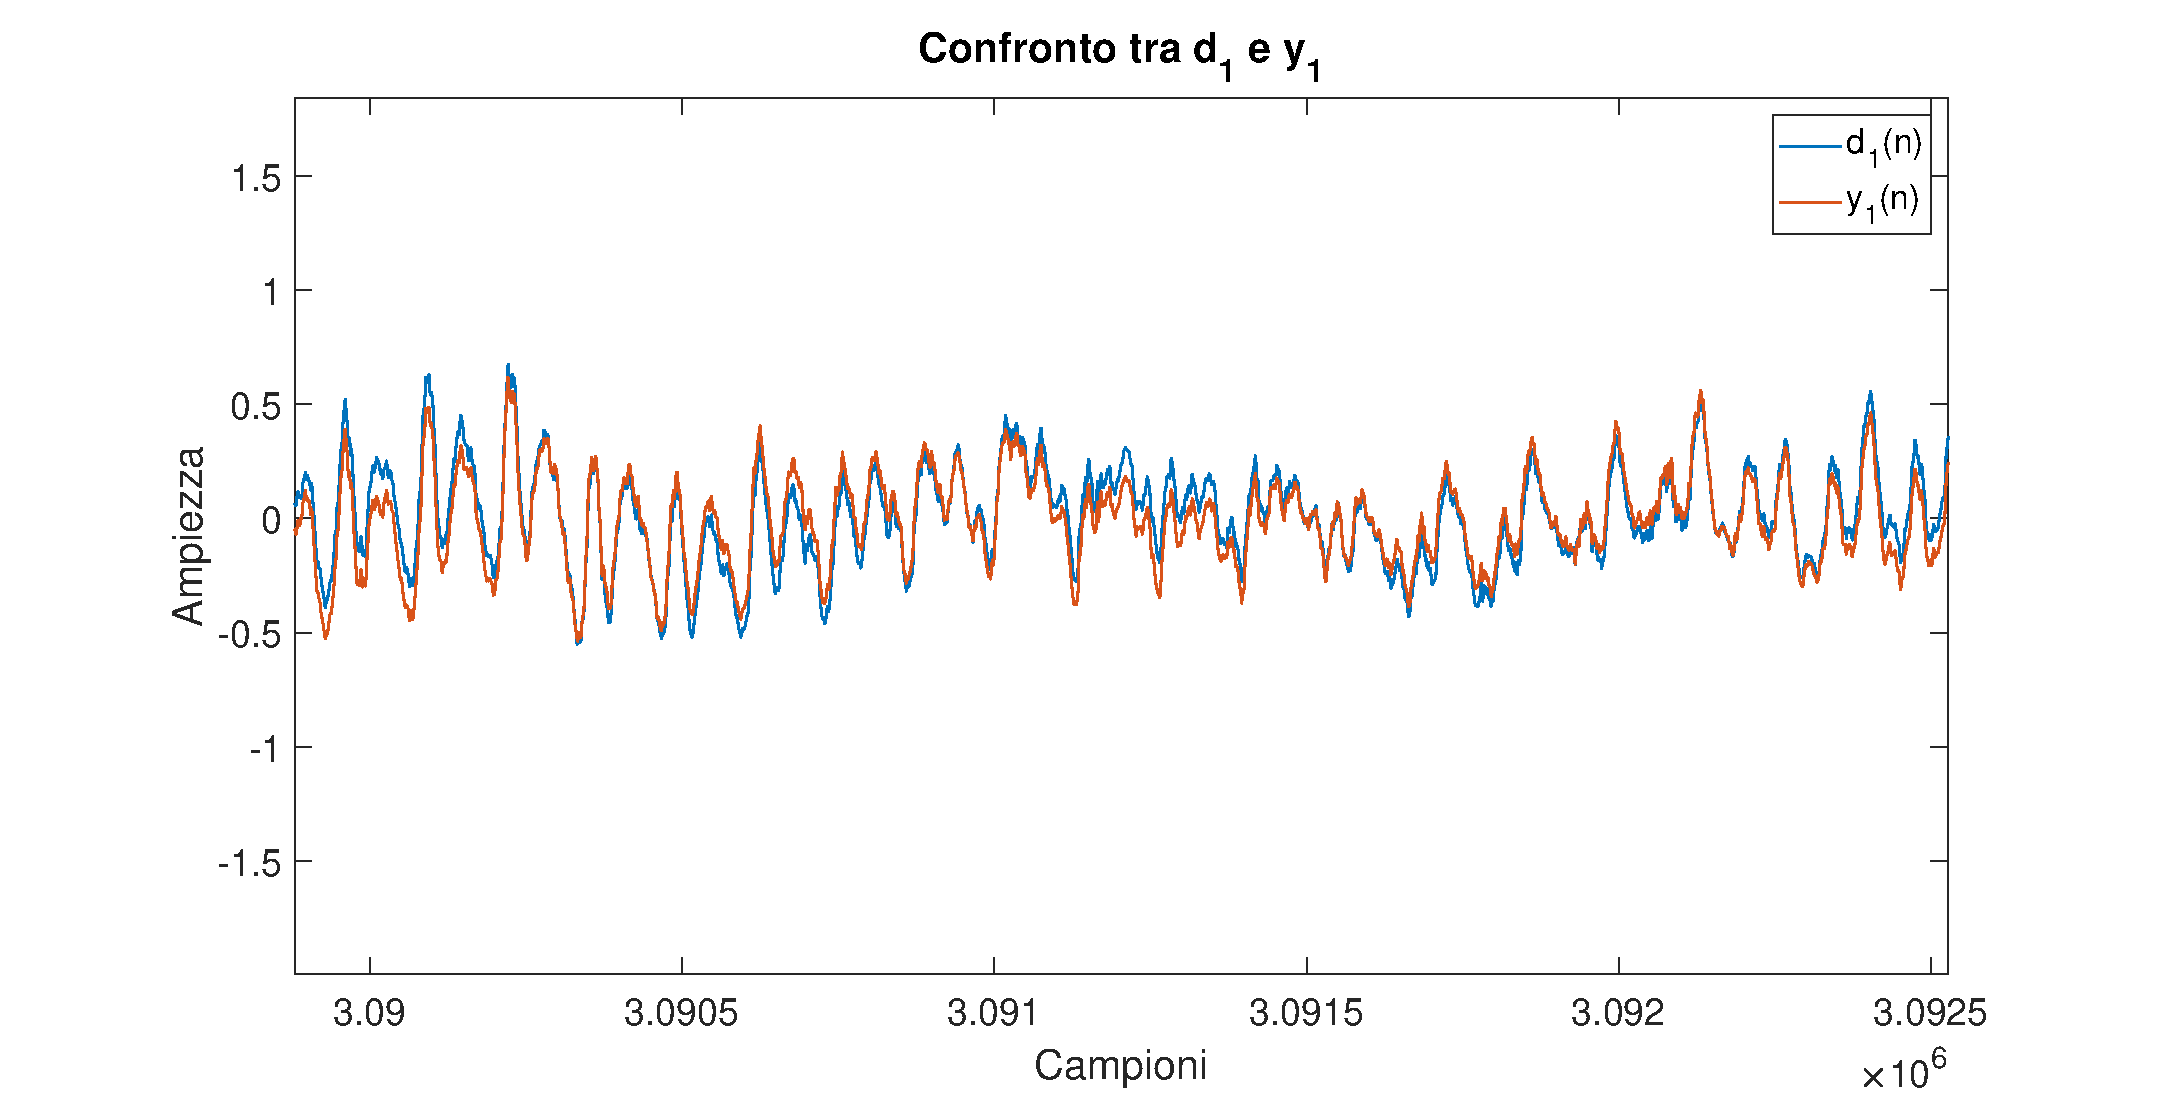
\includegraphics[width=1\textwidth]{Immagini/d1_y1_LMS}
		\caption{}
		\label{fig:d1_y1_LMS}
	\end{subfigure}\\
	\begin{subfigure}{1\textwidth}
		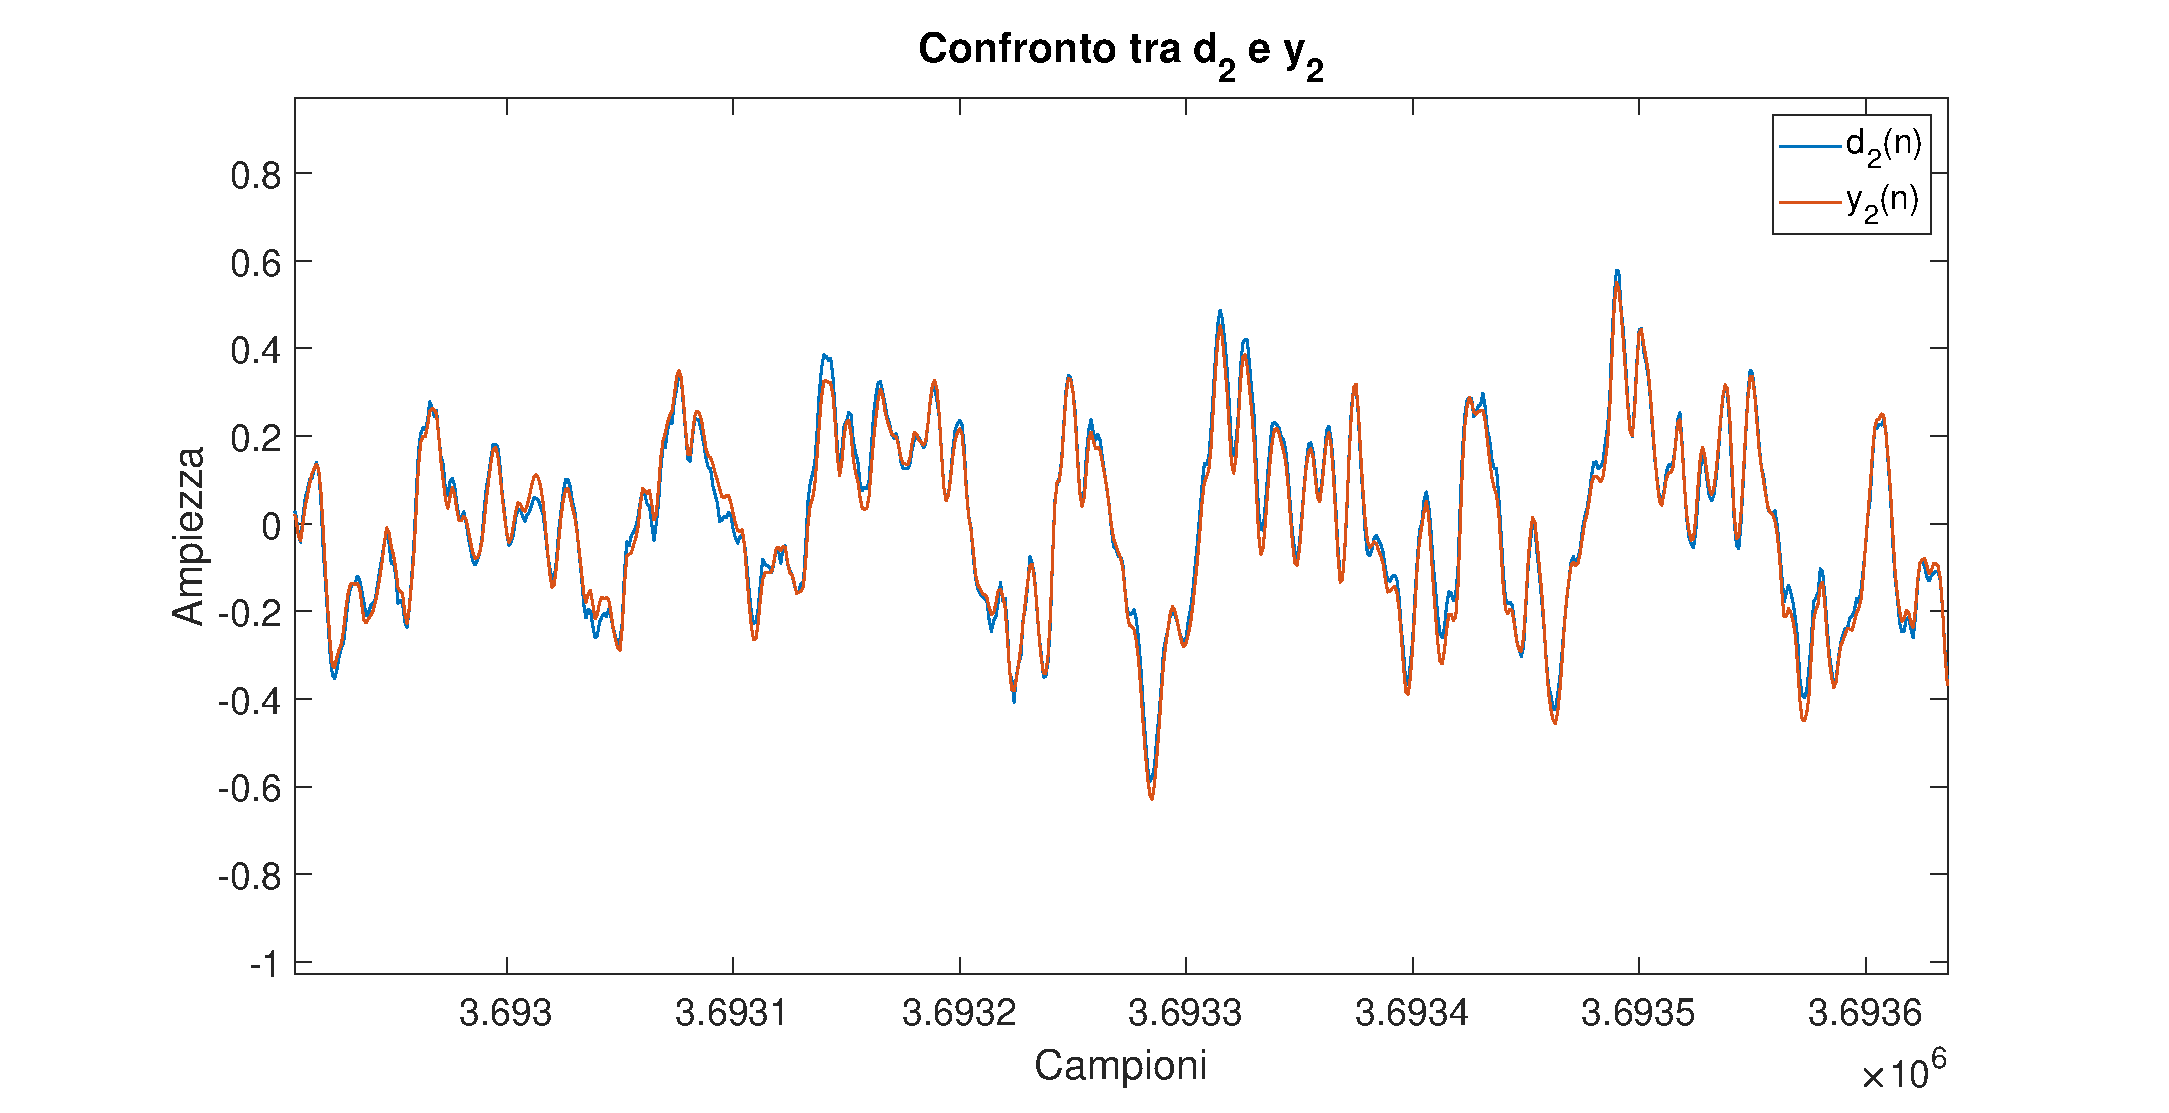
\includegraphics[width=1\textwidth]{Immagini/d2_y2_LMS}
		\caption{}
		\label{fig:d2_y2_LMS}
	\end{subfigure}
	\caption{Confronto degli ingressi e le uscite (a) sinistro e (b) destro della Fast Deconvolution, (c) sinistro e (d) destro di LMS.}
	\label{fig:confronto_ingressi_uscite_LMS_FD}
\end{figure}

I risultati ottenuti per ognuno dei due algoritmi con il NU-Tech sono uguali a quelli prodotti dal Matlab, questo ci permette di affermare che gli algoritmi sviluppati nei due diversi linguaggi di programmazione sono equivalenti e producono le stesse uscite.
\clearpage
\subsection{Risultati NU-Tech}
\label{subsec:risultati_nutech}
Per confermare la correttezza dei programmi sviluppati in NU-Tech, sono confrontati i risultati ottenuti con quelli precedentemente descritti in Matlab. Le figure~\ref{fig:lms_template_nutech} e~\ref{fig:fd_template_nutech} mostrano come sono collegati i NUTS che eseguono rispettivamente l'algoritmo LMS e FD nel NU-Tech. Nella figura~\ref{fig:lms_template_nutech} si può notare un blocco ``ADelay'' in cui viene inserito un ritardo nel segnale di ingresso, necessario per visualizzare e confrontare con il ``Viewer Mch'' il segnale desiderato, cioè l'ingresso ritardato, e l'uscita.

\begin{figure}[h]
	\centering
	\begin{subfigure}{1\textwidth}
		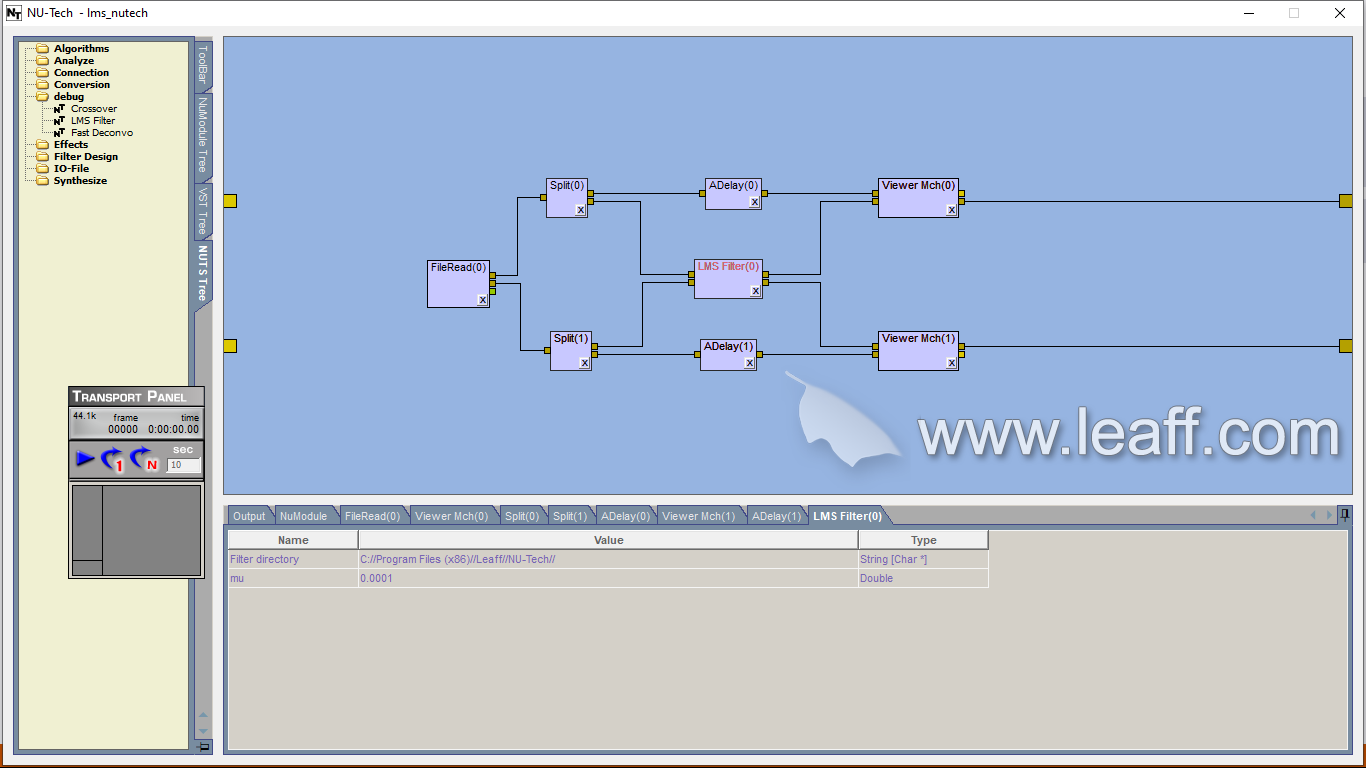
\includegraphics[width=1\textwidth]{Immagini/lms_template_nutech}
		\caption{}
		\label{fig:lms_template_nutech}
	\end{subfigure}\\
	\begin{subfigure}{1\textwidth}
			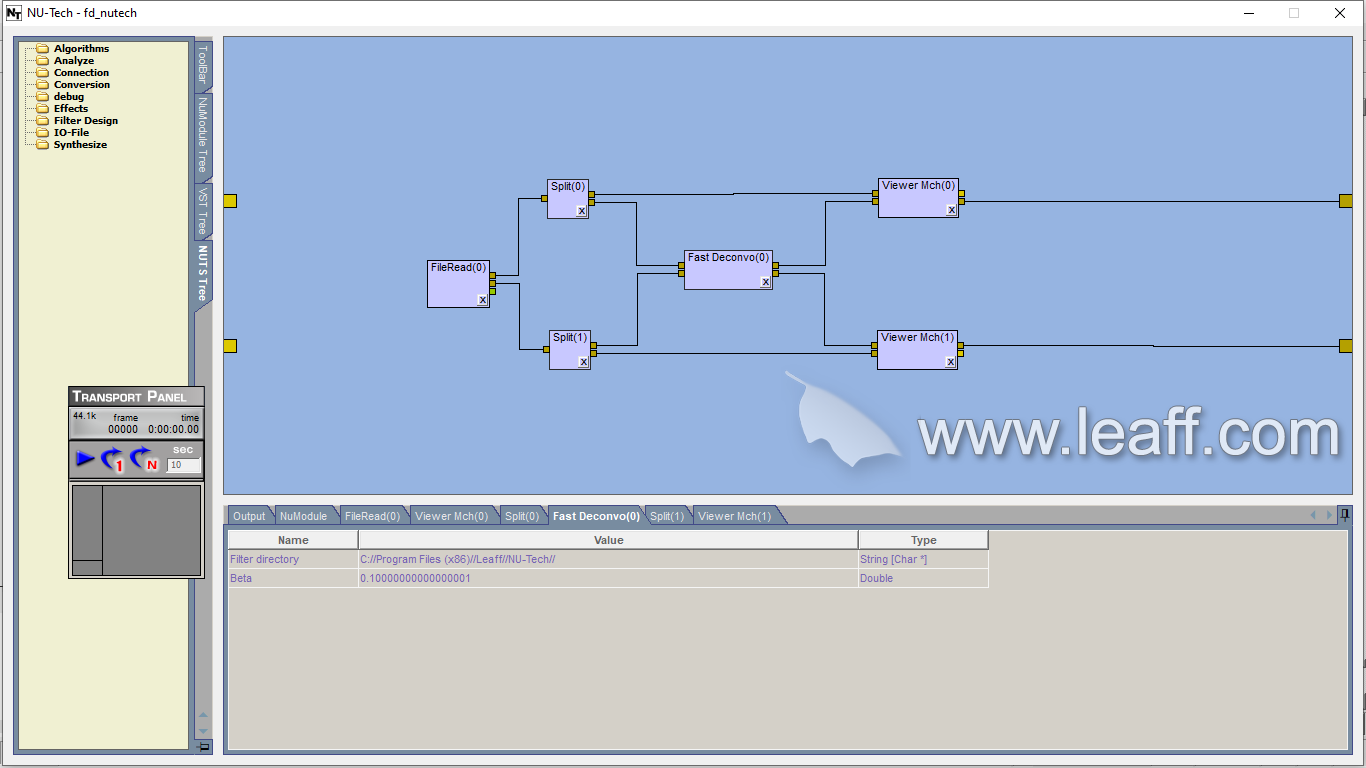
\includegraphics[width=1\textwidth]{Immagini/fd_template_nutech}
			\caption{}
			\label{fig:fd_template_nutech}
	\end{subfigure}
	\caption{Board del NU-Tech per l'algoritmo (a) LMS e (b) Fast Deconvolution.}
	\label{fig:template_nutech}
\end{figure}

Le figure~\ref{fig:x1_y1_FD_nutech} e~\ref{fig:x2_y2_FD_nutech} mostrano il confronto tra l'uscita e il segnale di ingresso per l'algoritmo Fast Deconvolution rispettivamente per il canale sinistro e destro, mentre~\ref{fig:d1_y1_LMS_nutech} e~\ref{fig:d2_y2_LMS_nutech} mostrano il confronto tra l'uscita e il segnale desiderato per l'algoritmo LMS rispettivamente per il canale sinistro e destro. Il segnale blu mostra il segnale di ingresso, mentre il segnale verde il segnale all'uscita del NUTS. Confrontando queste quattro figure rispettivamente con~\ref{fig:x1_y1_FD},~\ref{fig:x2_y2_FD},~\ref{fig:d1_y1_LMS} e~\ref{fig:d2_y2_LMS} dell'algoritmo in Matlab si può vedere che hanno lo stesso andamento.
\begin{figure}[h]
	\centering
	\begin{subfigure}{1\textwidth}
		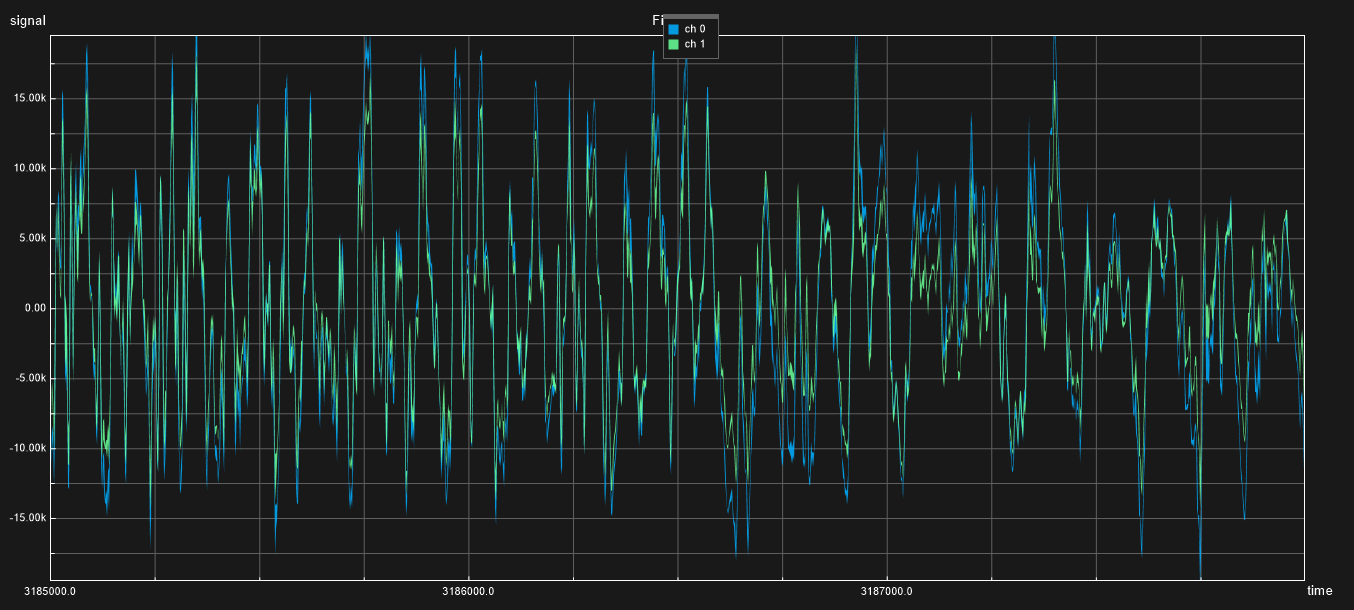
\includegraphics[width=1\textwidth]{Immagini/x1_y1_FD_nutech}
		\caption{}
		\label{fig:x1_y1_FD_nutech}
	\end{subfigure}\\
	\begin{subfigure}{1\textwidth}
			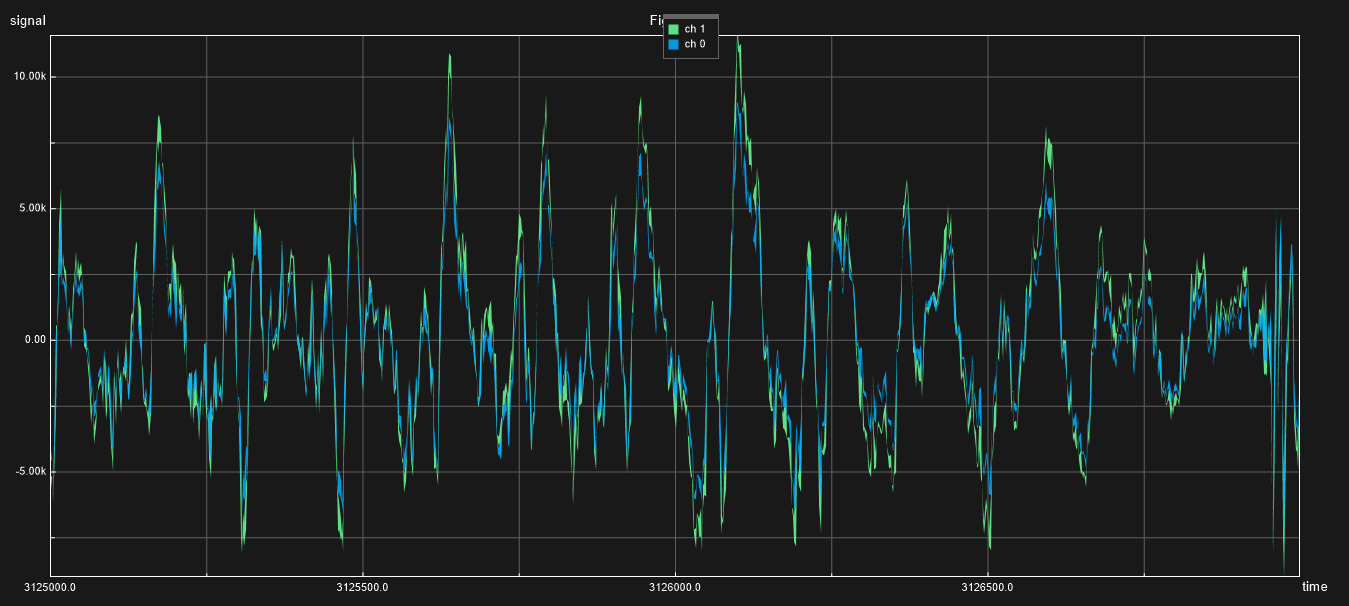
\includegraphics[width=1\textwidth]{Immagini/x2_y2_FD_nutech}
			\caption{}
			\label{fig:x2_y2_FD_nutech}
	\end{subfigure}
\end{figure}

\begin{figure}[h]
	\ContinuedFloat
	\centering
	\begin{subfigure}{1\textwidth}
		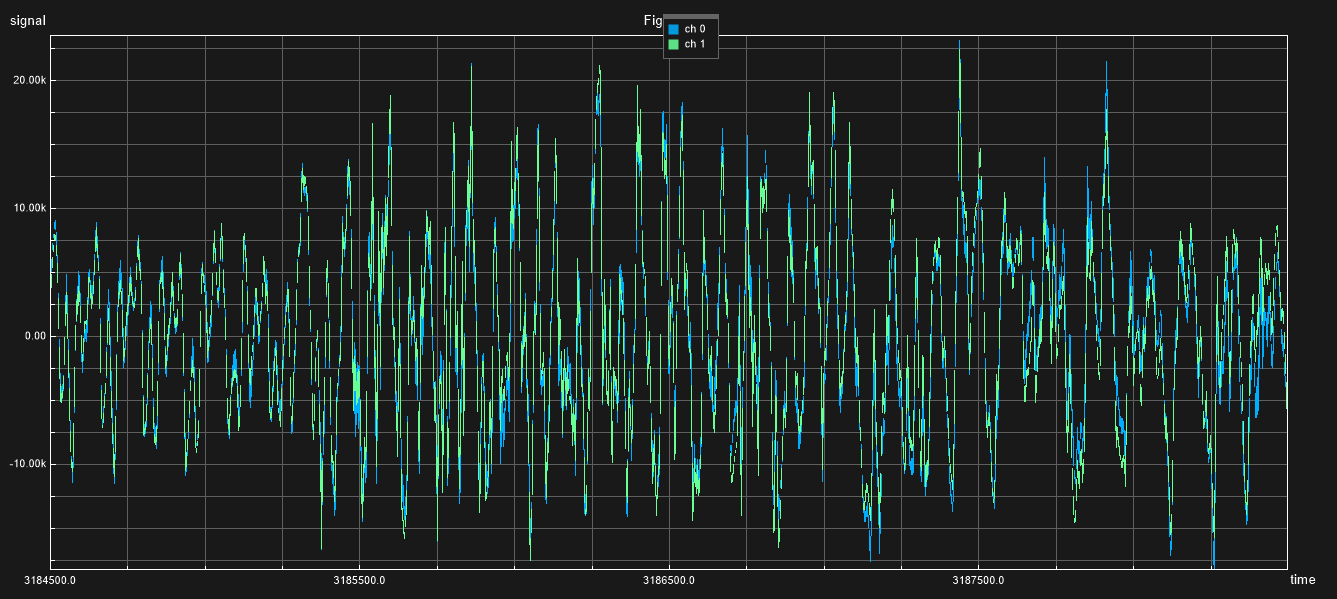
\includegraphics[width=1\textwidth]{Immagini/d1_y1_LMS_nutech}
		\caption{}
		\label{fig:d1_y1_LMS_nutech}
	\end{subfigure}\\
	\begin{subfigure}{1\textwidth}
		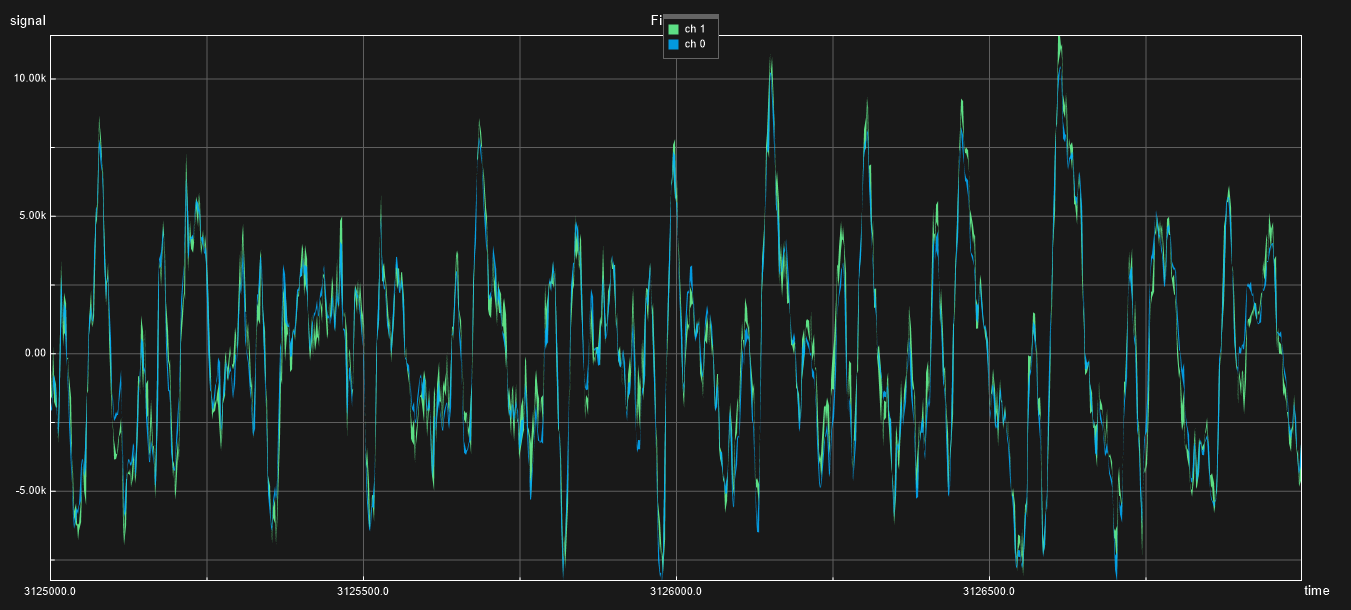
\includegraphics[width=1\textwidth]{Immagini/d2_y2_LMS_nutech}
		\caption{}
		\label{fig:d2_y2_LMS_nutech}
	\end{subfigure}
		\caption{Confronto degli ingressi e le uscite (a) sinistro e (b) destro della Fast Deconvolution, (c) sinistro e (d) destro di LMS.}
		\label{fig:confronto_ingressi_uscita_LMS_nutech}
\end{figure}

Le figure~\ref{fig:mse_e1_matlab_nutech} e~\ref{fig:mse_e2_matlab_nutech} illustrano l'andamento nel tempo del mean square error in \si{\decibel} dell'algoritmo LMS implementato in Matlab e in NU-Tech rappresentato da una linea tratteggiata rispettivamente blu e rossa. Si può notare che le due linee si sovrappongono dato che i due algoritmi implementati nei due linguaggi di programmazione si equivalgono.
\begin{figure}[h]
	\centering
	\begin{subfigure}{1\textwidth}
		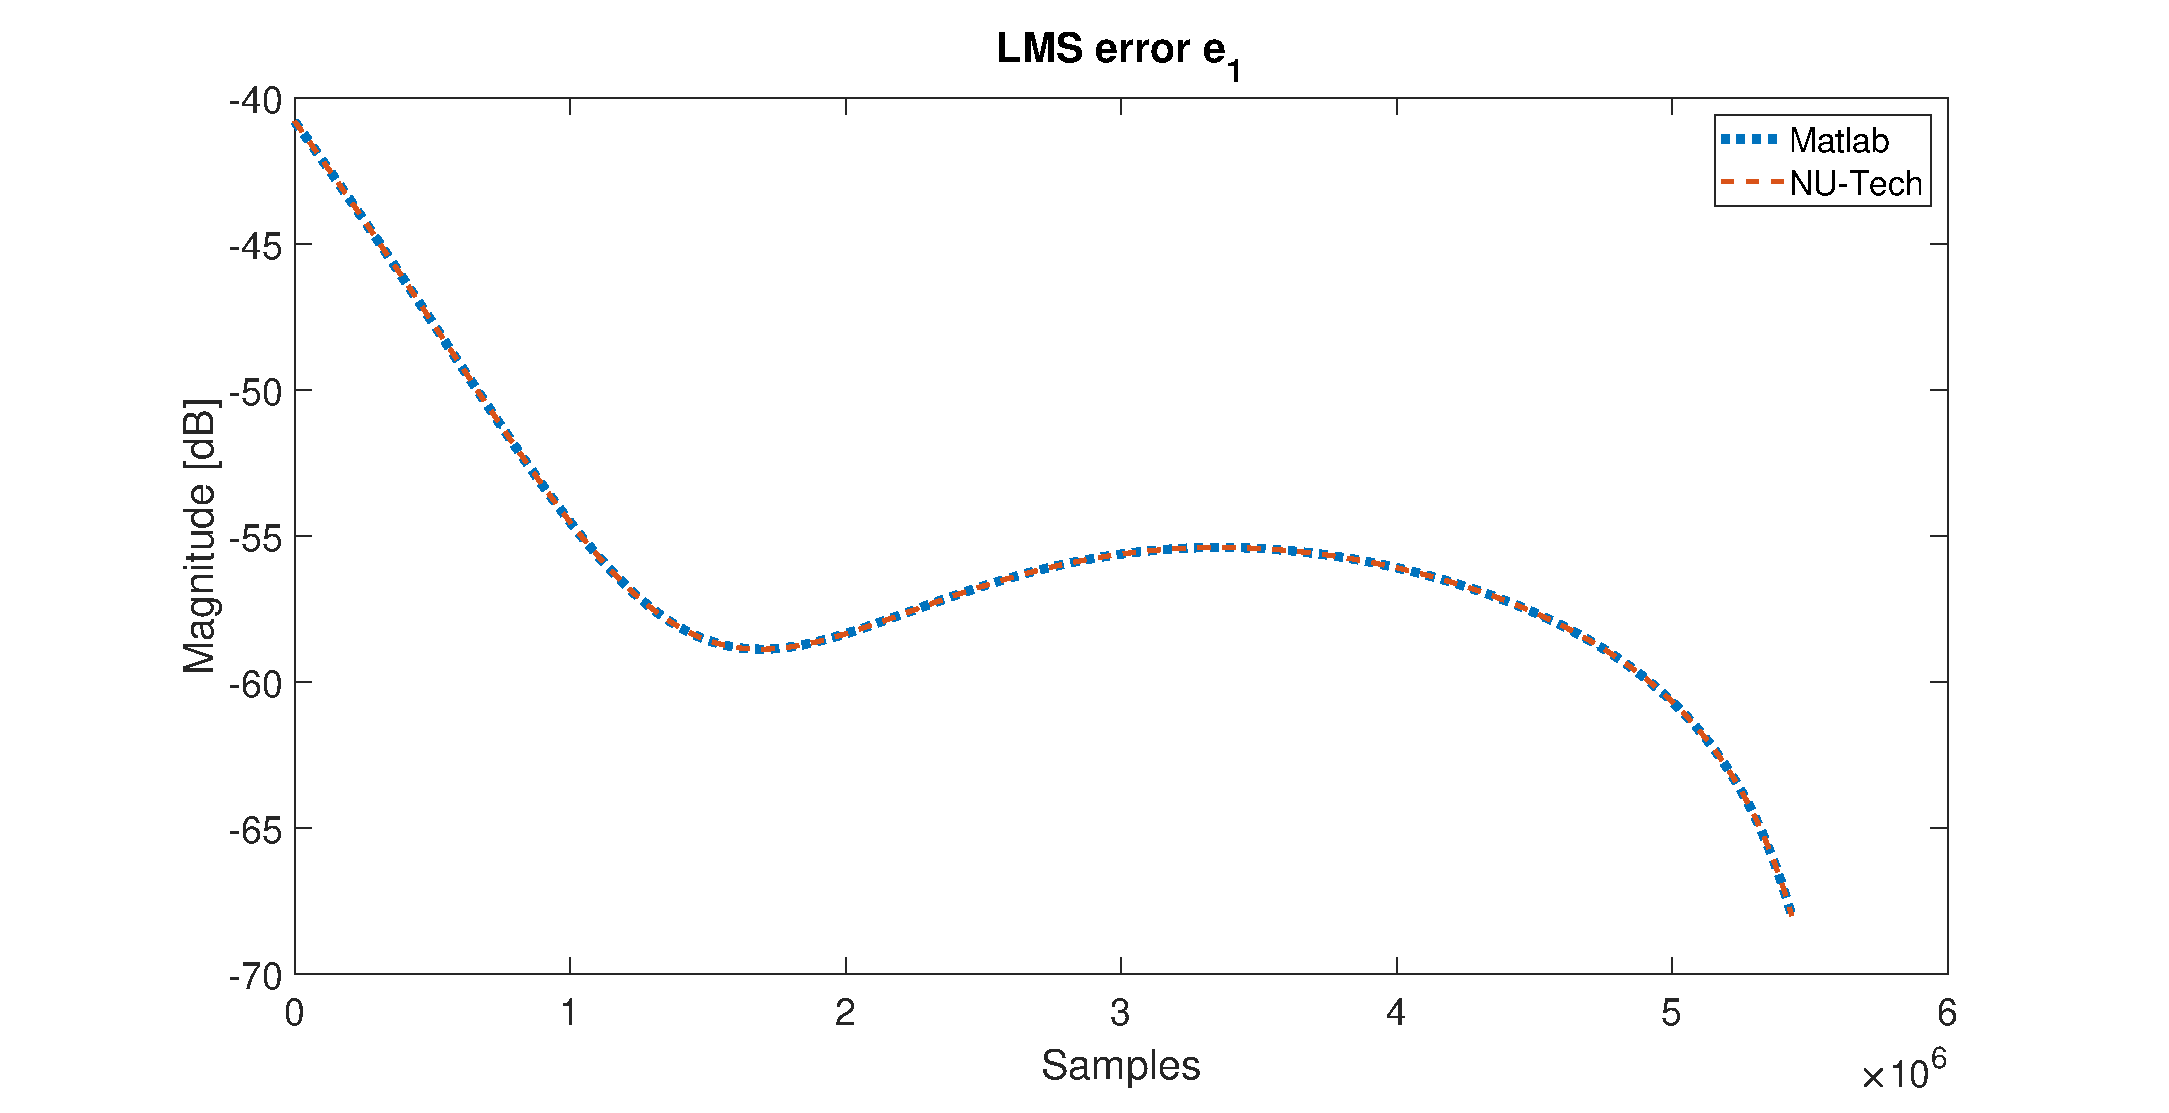
\includegraphics[width=1\textwidth]{Immagini/mse_e1_matlab_nutech}
		\caption{}
		\label{fig:mse_e1_matlab_nutech}
	\end{subfigure}\\
	\begin{subfigure}{1\textwidth}
			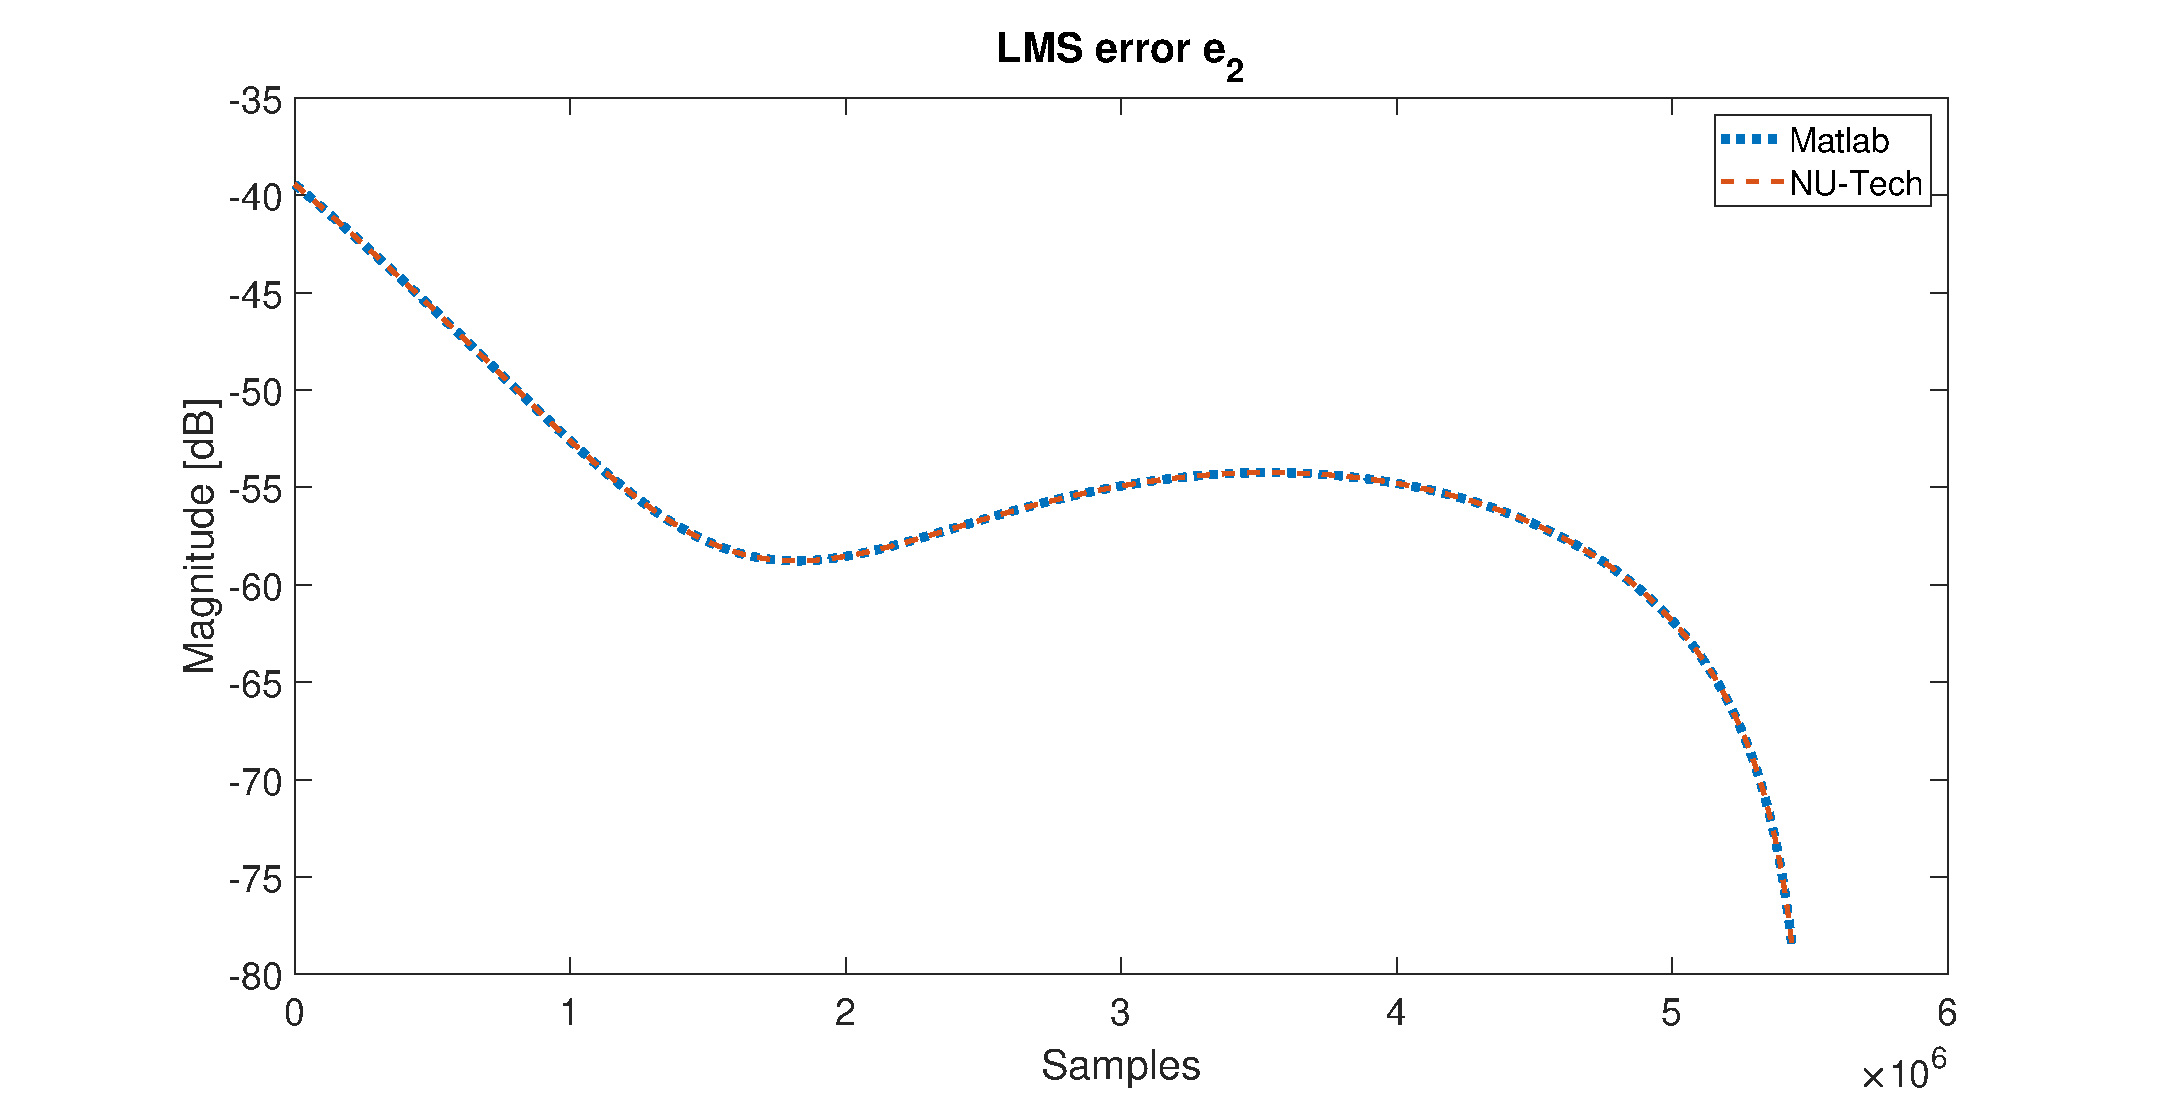
\includegraphics[width=1\textwidth]{Immagini/mse_e2_matlab_nutech}
			\caption{}
			\label{fig:mse_e2_matlab_nutech}
	\end{subfigure}
	\caption{Confronto dell'MSE del canale (a) sinistro e (b) destro dell'algoritmo LMS.}
	\label{fig:mse_matlab_nutech}
\end{figure}

Le figure~\ref{fig:H11_LMS_matlab_nutech},~\ref{fig:H12_LMS_matlab_nutech},~\ref{fig:H21_LMS_matlab_nutech} e~\ref{fig:H22_LMS_matlab_nutech} presentano rispettivamente un confronto tra i filtri di cancellazione del crosstalk  $H_{11}$, $H_{12}$, $H_{21}$ e $H_{22}$ ottenuti in Matlab, linea tratteggiata blu, e in NU-Tech, linea tratteggiata rossa, per l'algoritmo LMS.

Allo stesso modo, le figure~\ref{fig:H11_FD_matlab_nutech},~\ref{fig:H12_FD_matlab_nutech},~\ref{fig:H21_FD_matlab_nutech} e~\ref{fig:H22_FD_matlab_nutech} mostrano i filtri di cancellazione per l'algoritmo Fast Deconvolution. Anche in questo caso si può vedere che i grafici si sovrappongono a dimostrazione della validità di entrambi i programmi.
\begin{figure}[h]
	\centering
	\begin{subfigure}{1\textwidth}
		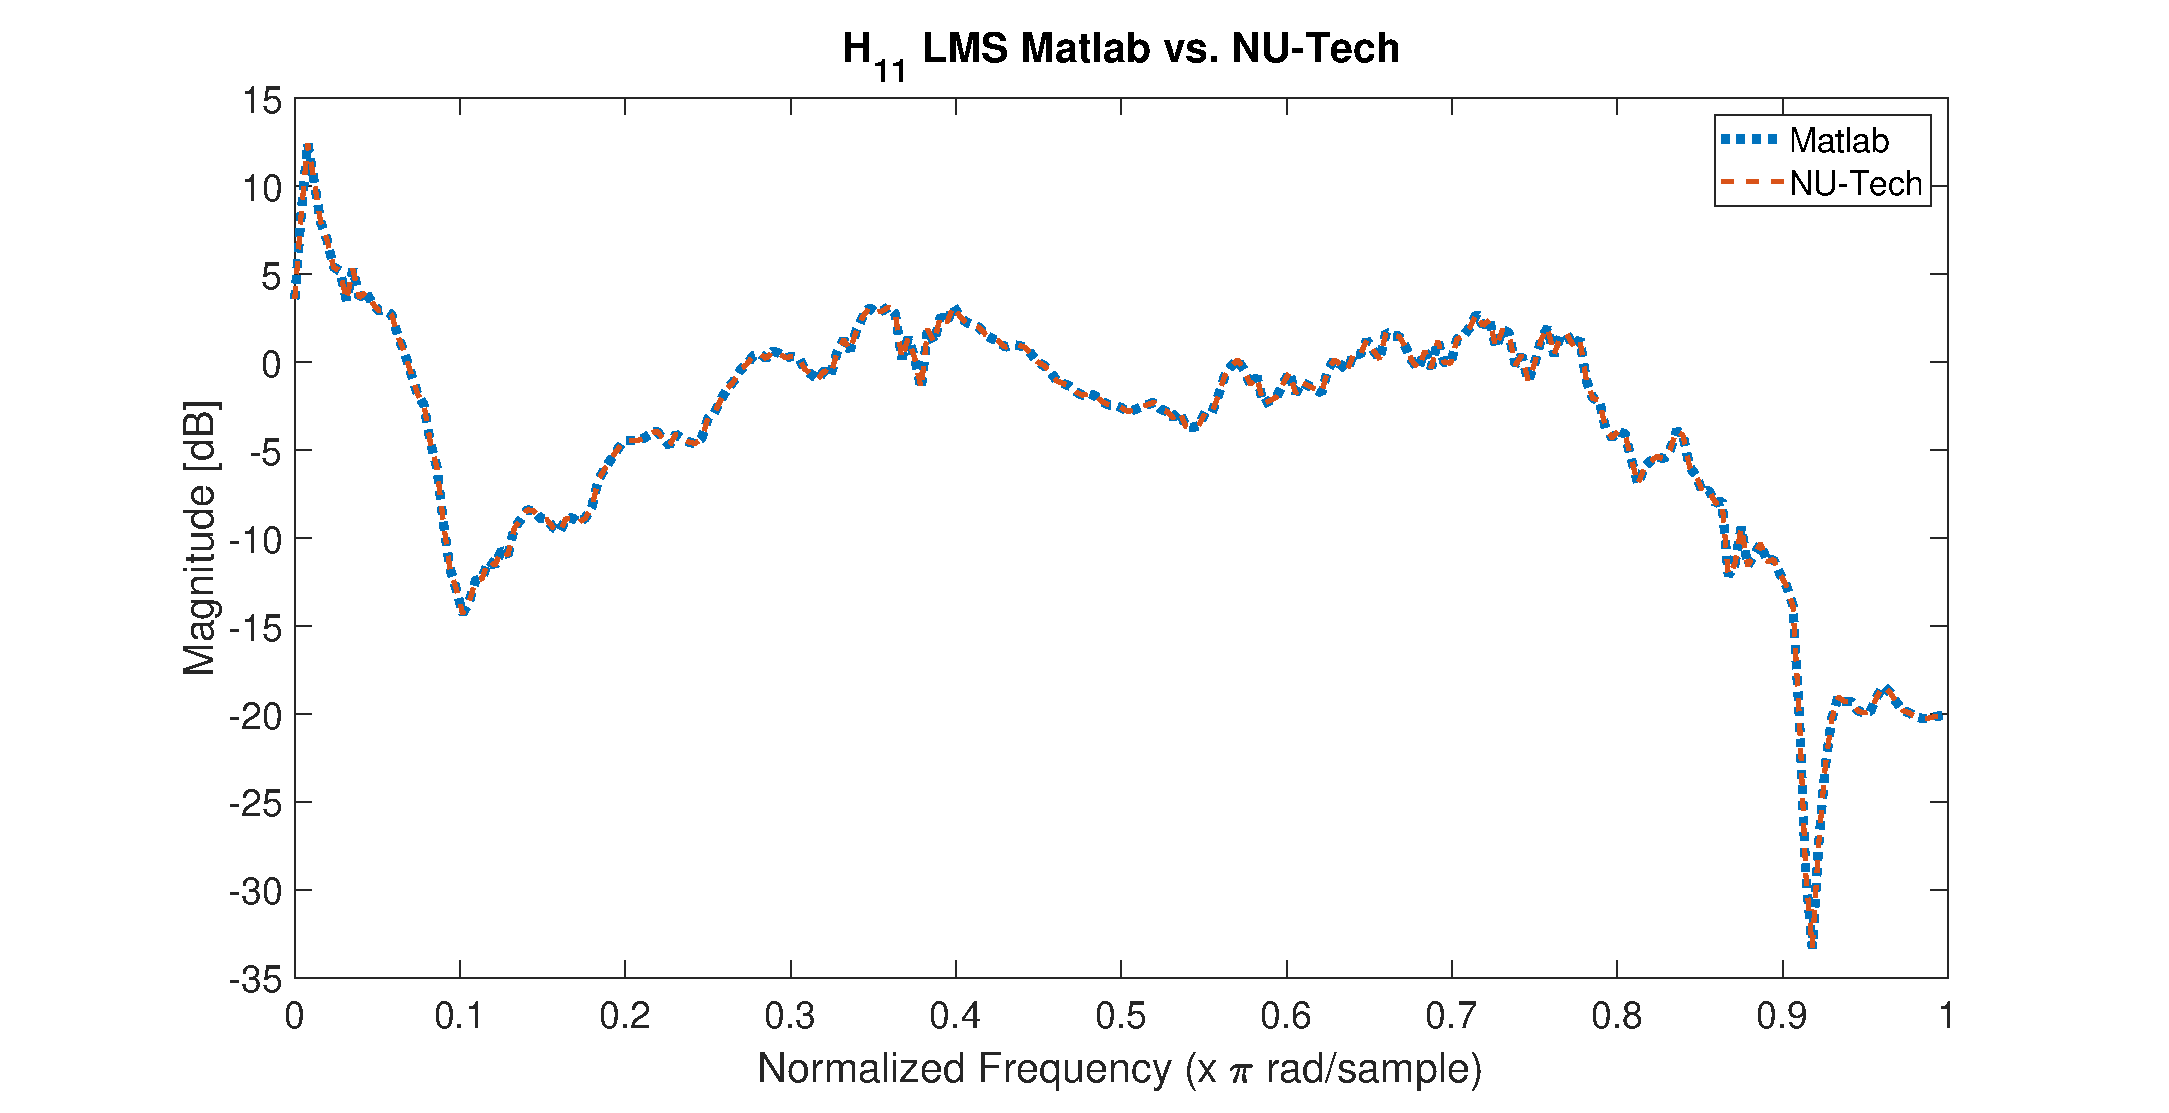
\includegraphics[width=1\textwidth]{Immagini/H11_LMS_matlab_nutech}
		\caption{}
		\label{fig:H11_LMS_matlab_nutech}
	\end{subfigure}\\
	\begin{subfigure}{1\textwidth}
			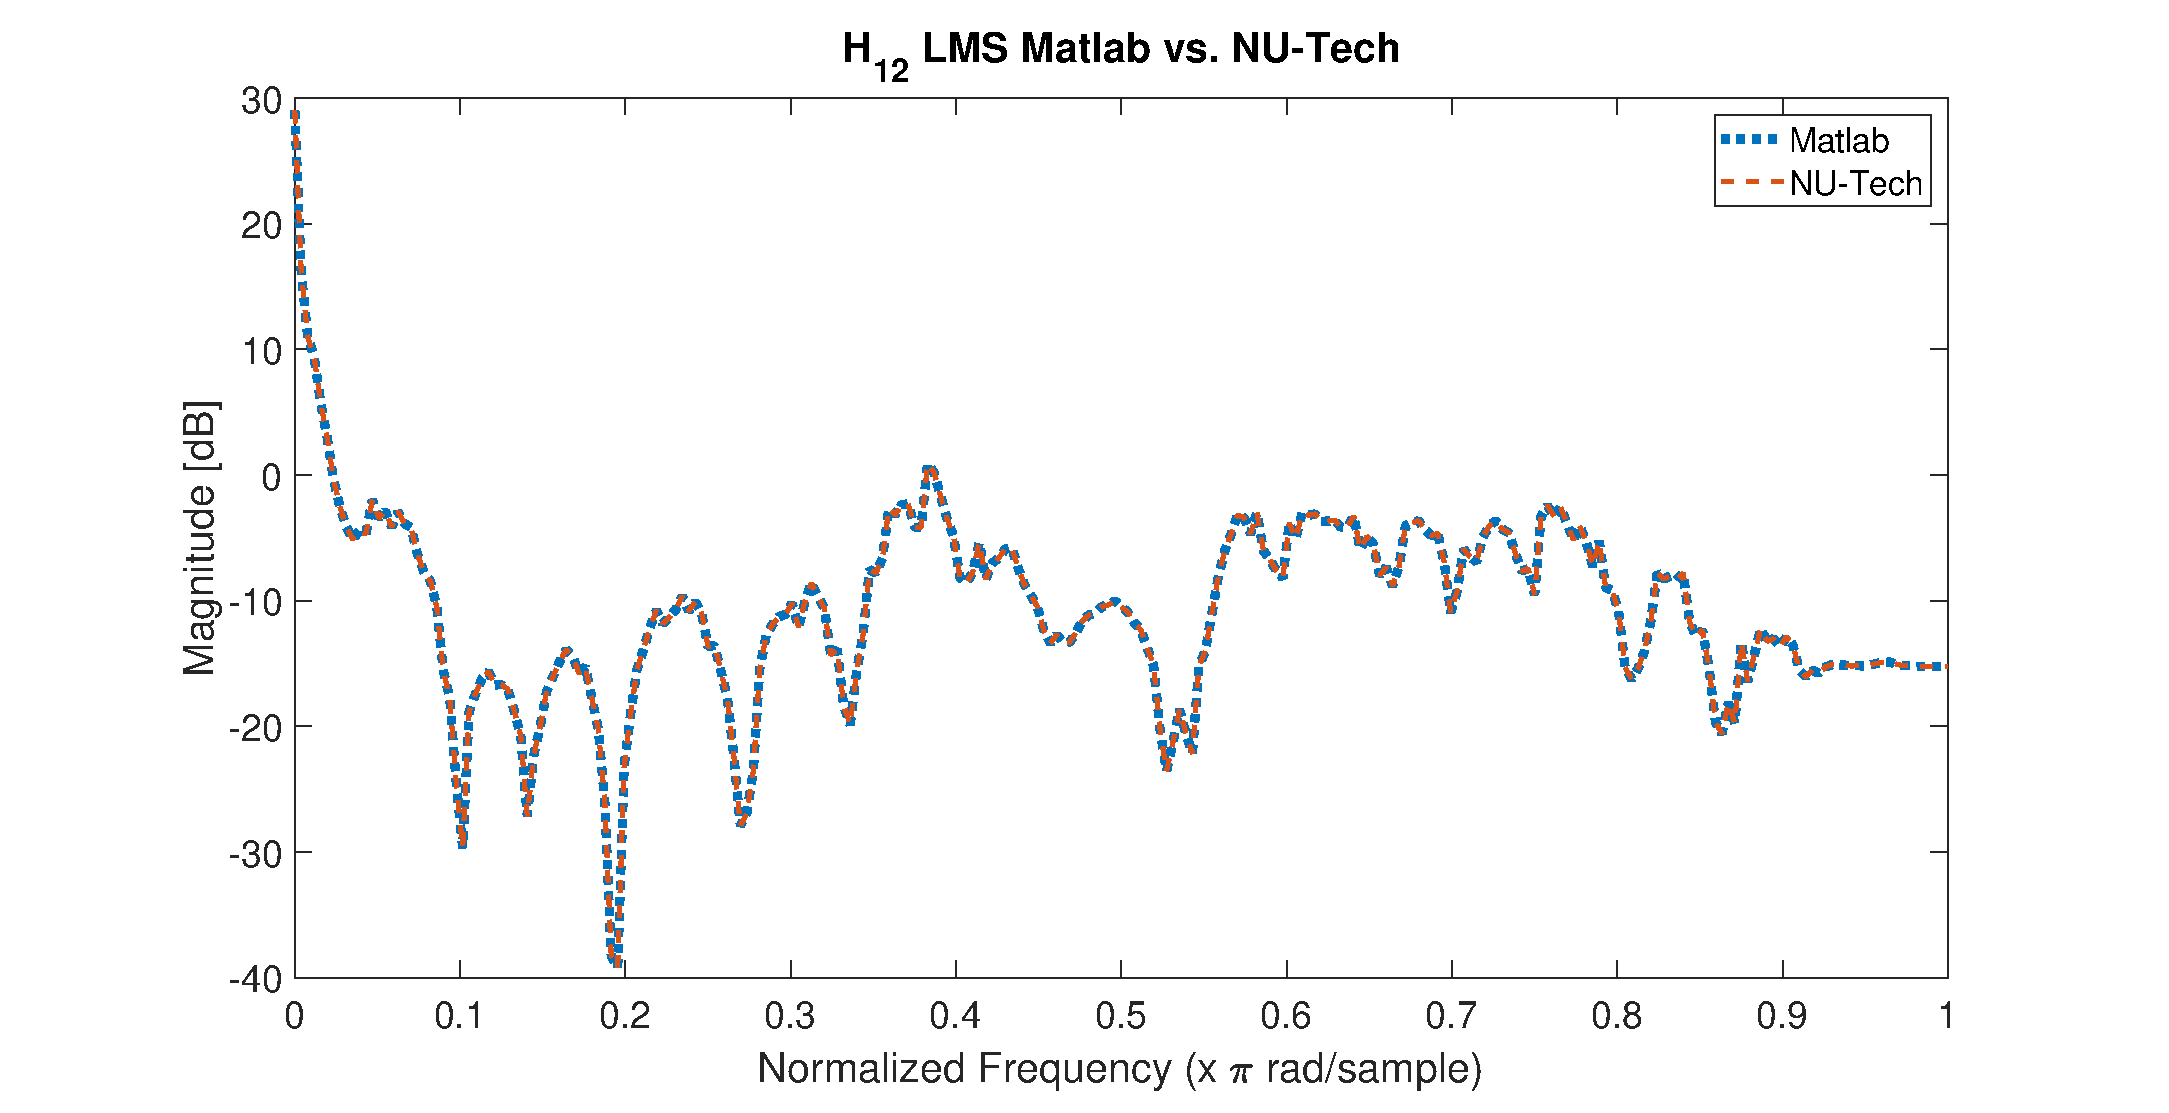
\includegraphics[width=1\textwidth]{Immagini/H12_LMS_matlab_nutech}
			\caption{}
			\label{fig:H12_LMS_matlab_nutech}
	\end{subfigure}
\end{figure}

\begin{figure}[h]
	\ContinuedFloat
	\centering
	\begin{subfigure}{1\textwidth}
		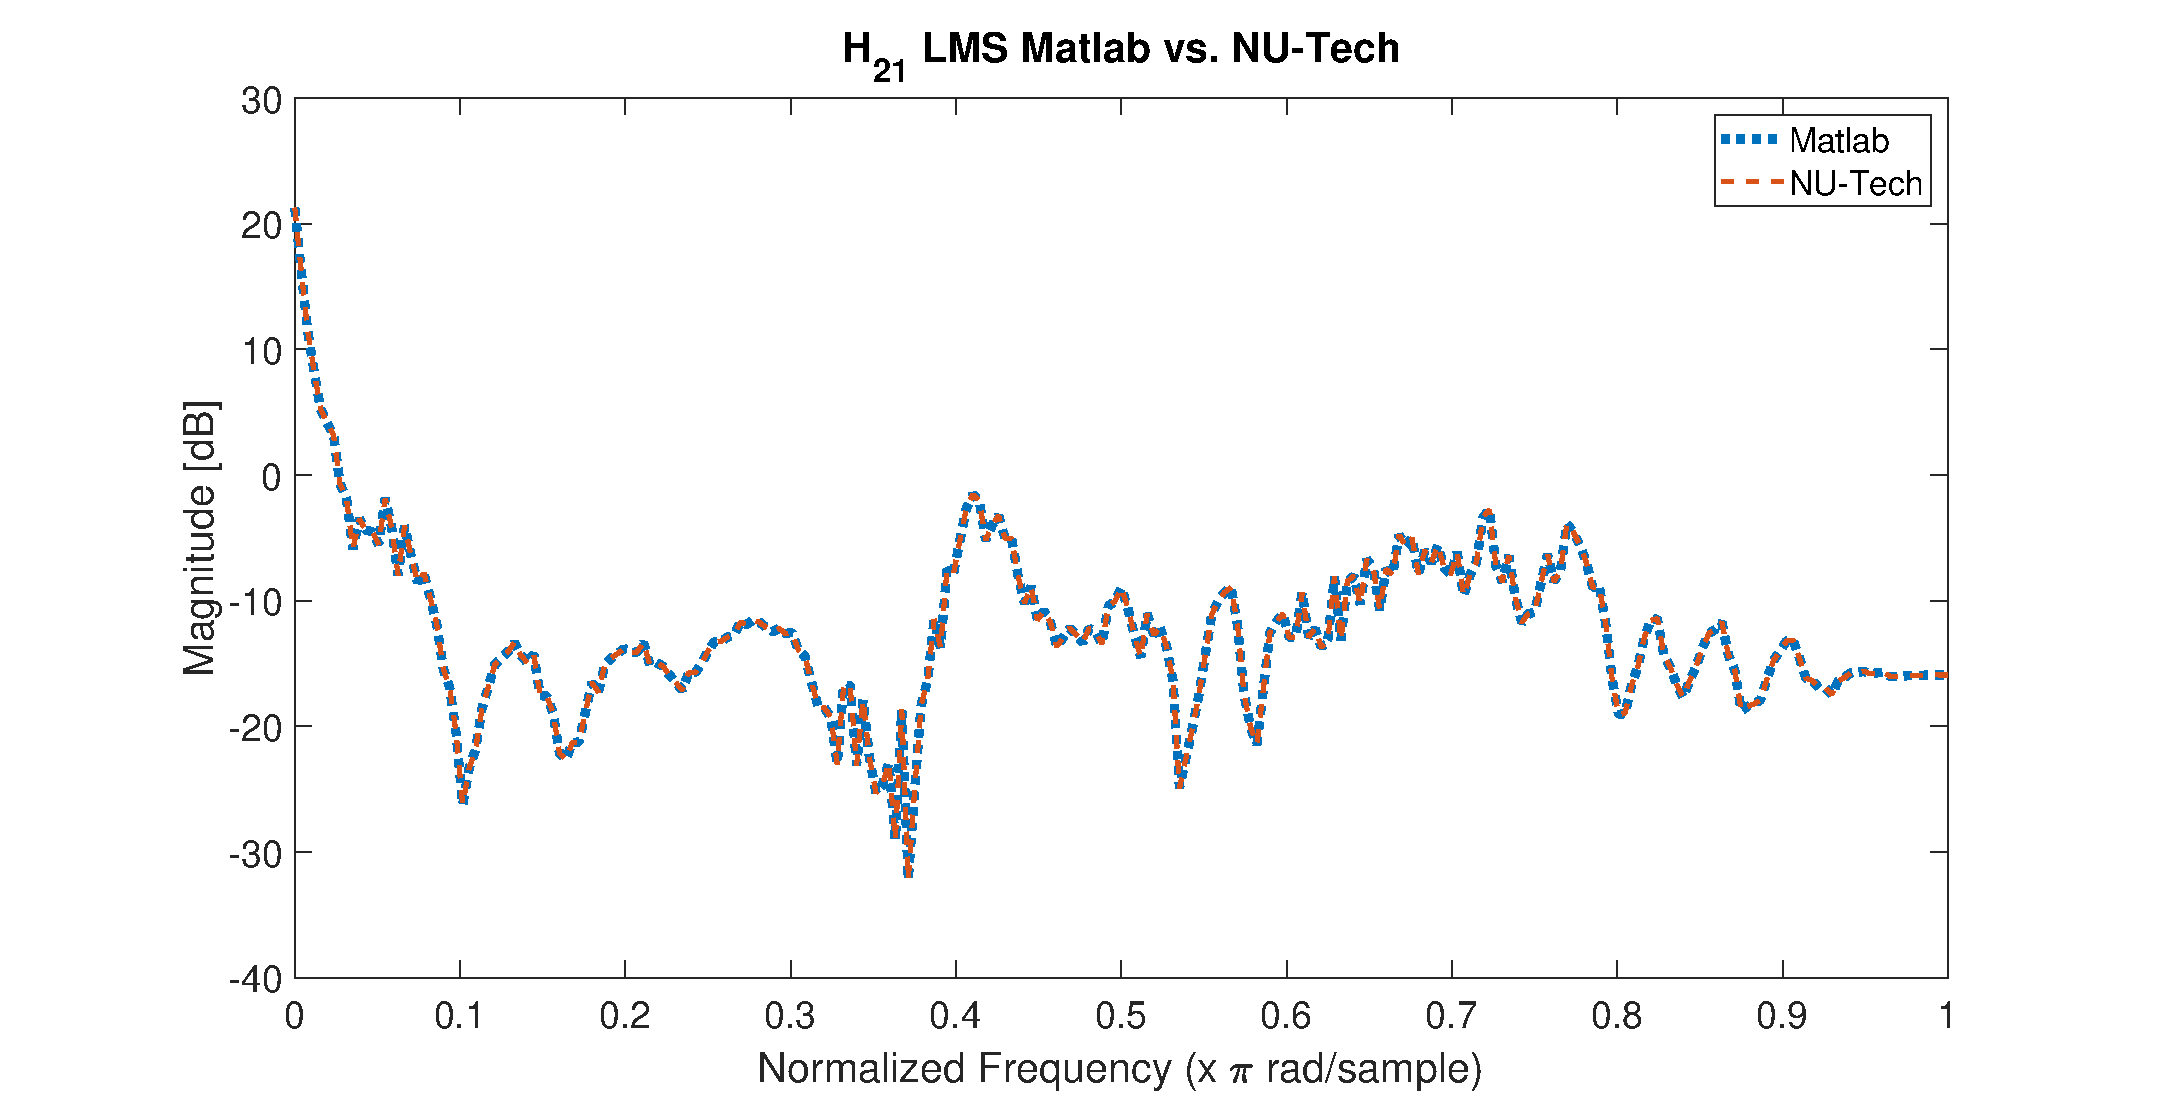
\includegraphics[width=1\textwidth]{Immagini/H21_LMS_matlab_nutech}
		\caption{}
		\label{fig:H21_LMS_matlab_nutech}
	\end{subfigure}\\
	\begin{subfigure}{1\textwidth}
		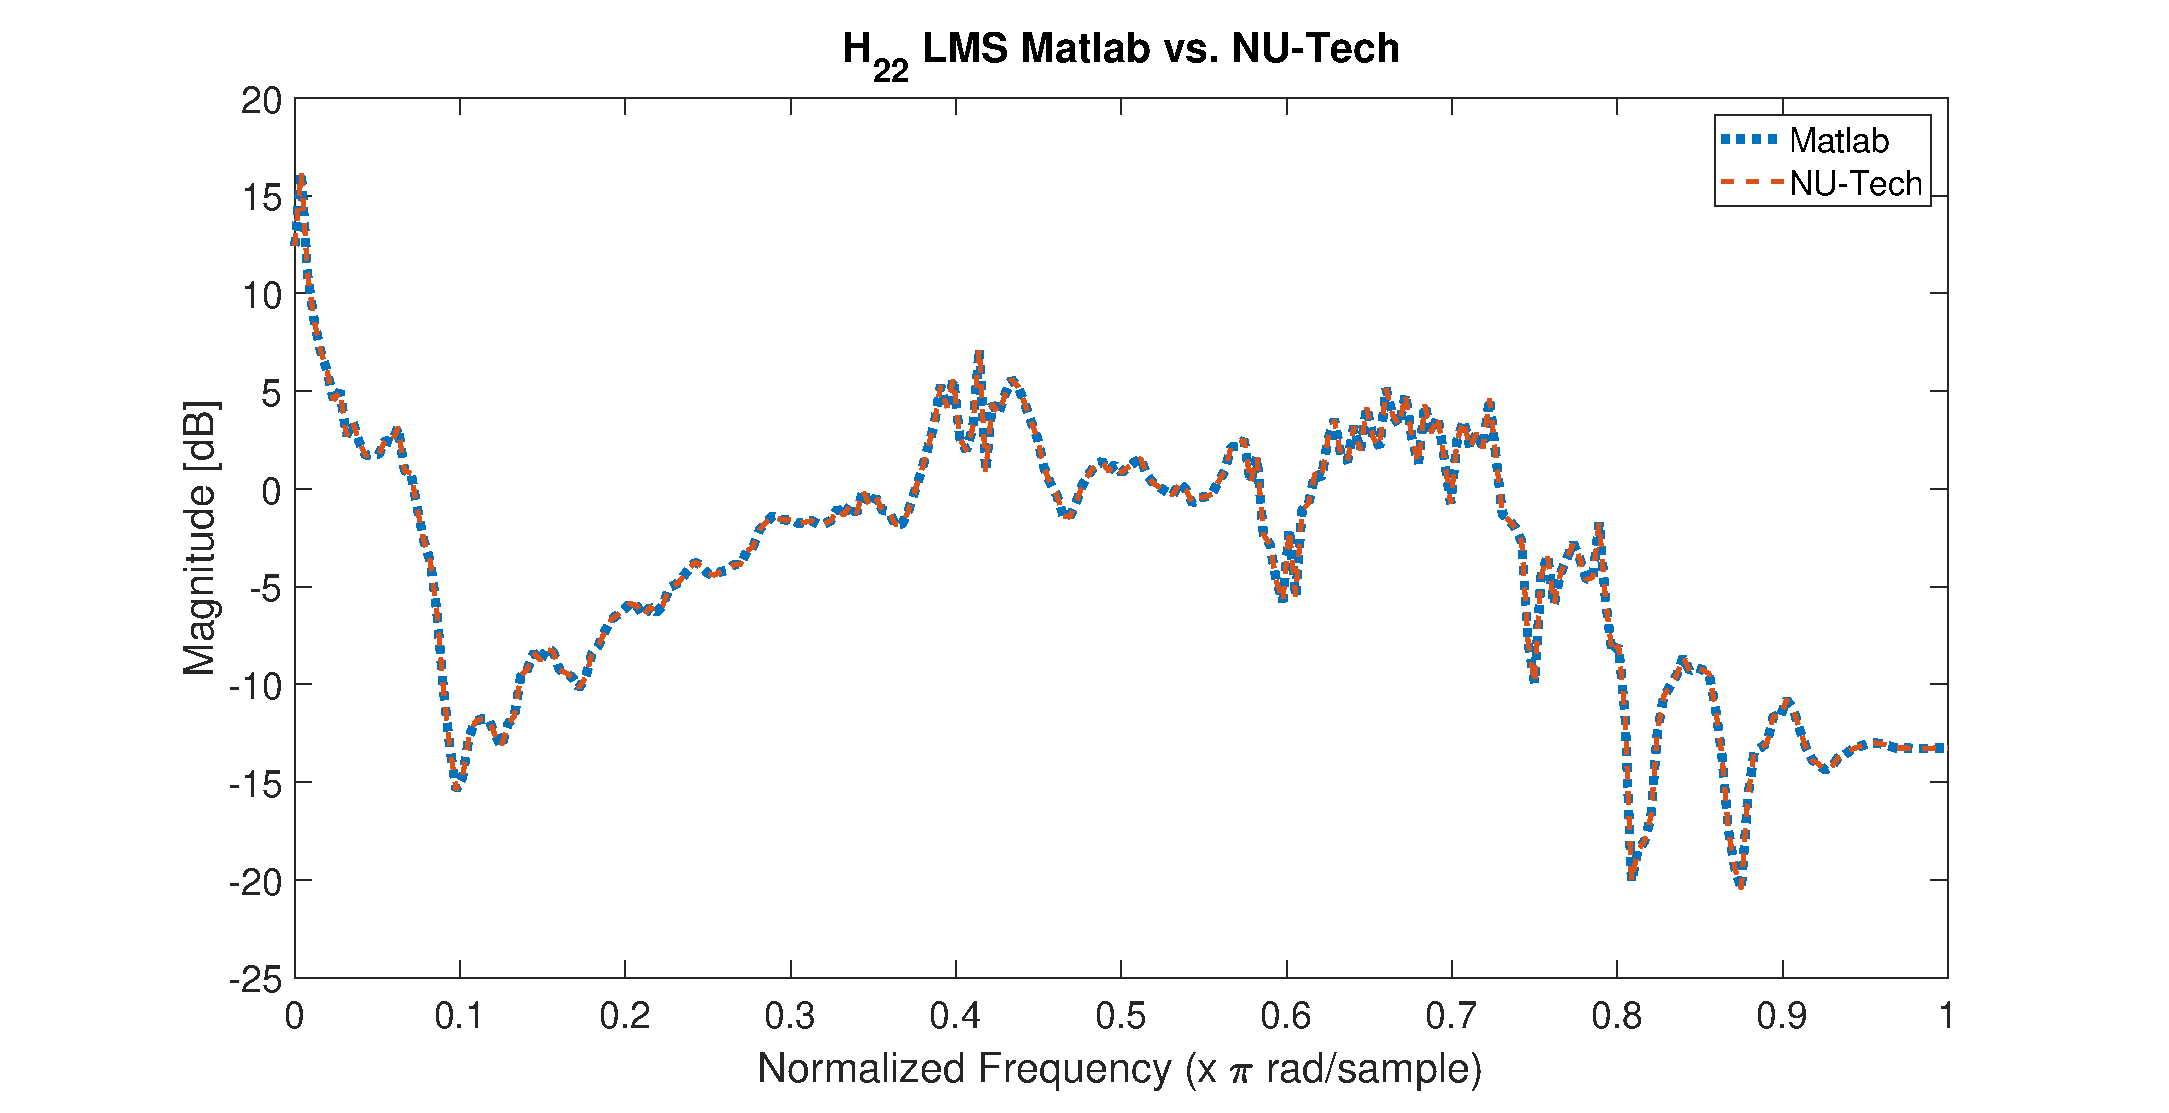
\includegraphics[width=1\textwidth]{Immagini/H22_LMS_matlab_nutech}
		\caption{}
		\label{fig:H22_LMS_matlab_nutech}
	\end{subfigure}
		\caption{Confronto dei filtri di cancellazione del crosstalk (a) $H_{11}$, (b) $H_{12}$, (c) $H_{21}$ e (d) $H_{22}$ in Matlab e in NU-Tech per l'algoritmo LMS.}
		\label{fig:confronto_filtri_matlab_nutech_lms}
\end{figure}

\begin{figure}[h]
	\centering
	\begin{subfigure}{1\textwidth}
		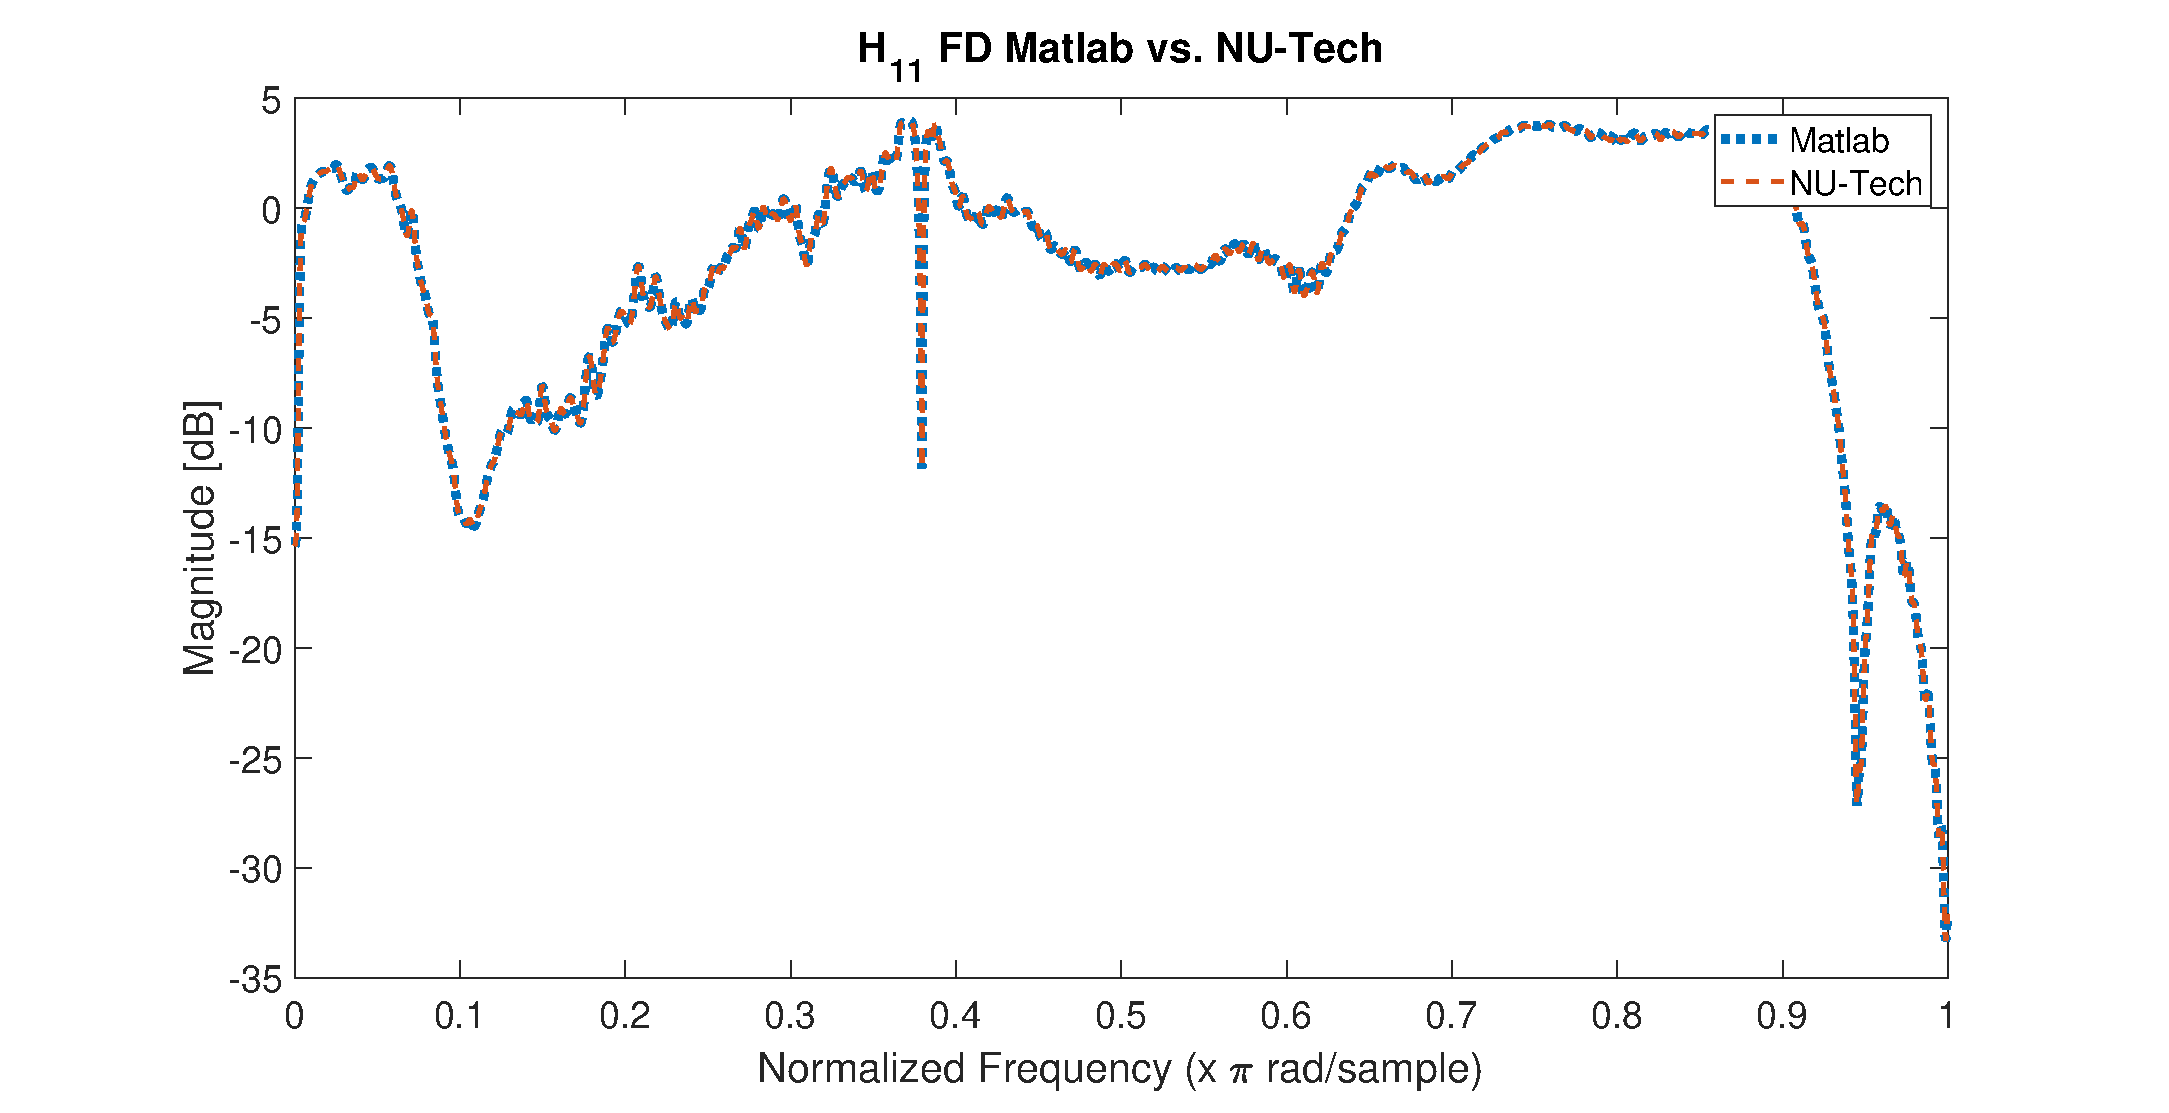
\includegraphics[width=1\textwidth]{Immagini/H11_FD_matlab_nutech}
		\caption{}
		\label{fig:H11_FD_matlab_nutech}
	\end{subfigure}\\
	\begin{subfigure}{1\textwidth}
			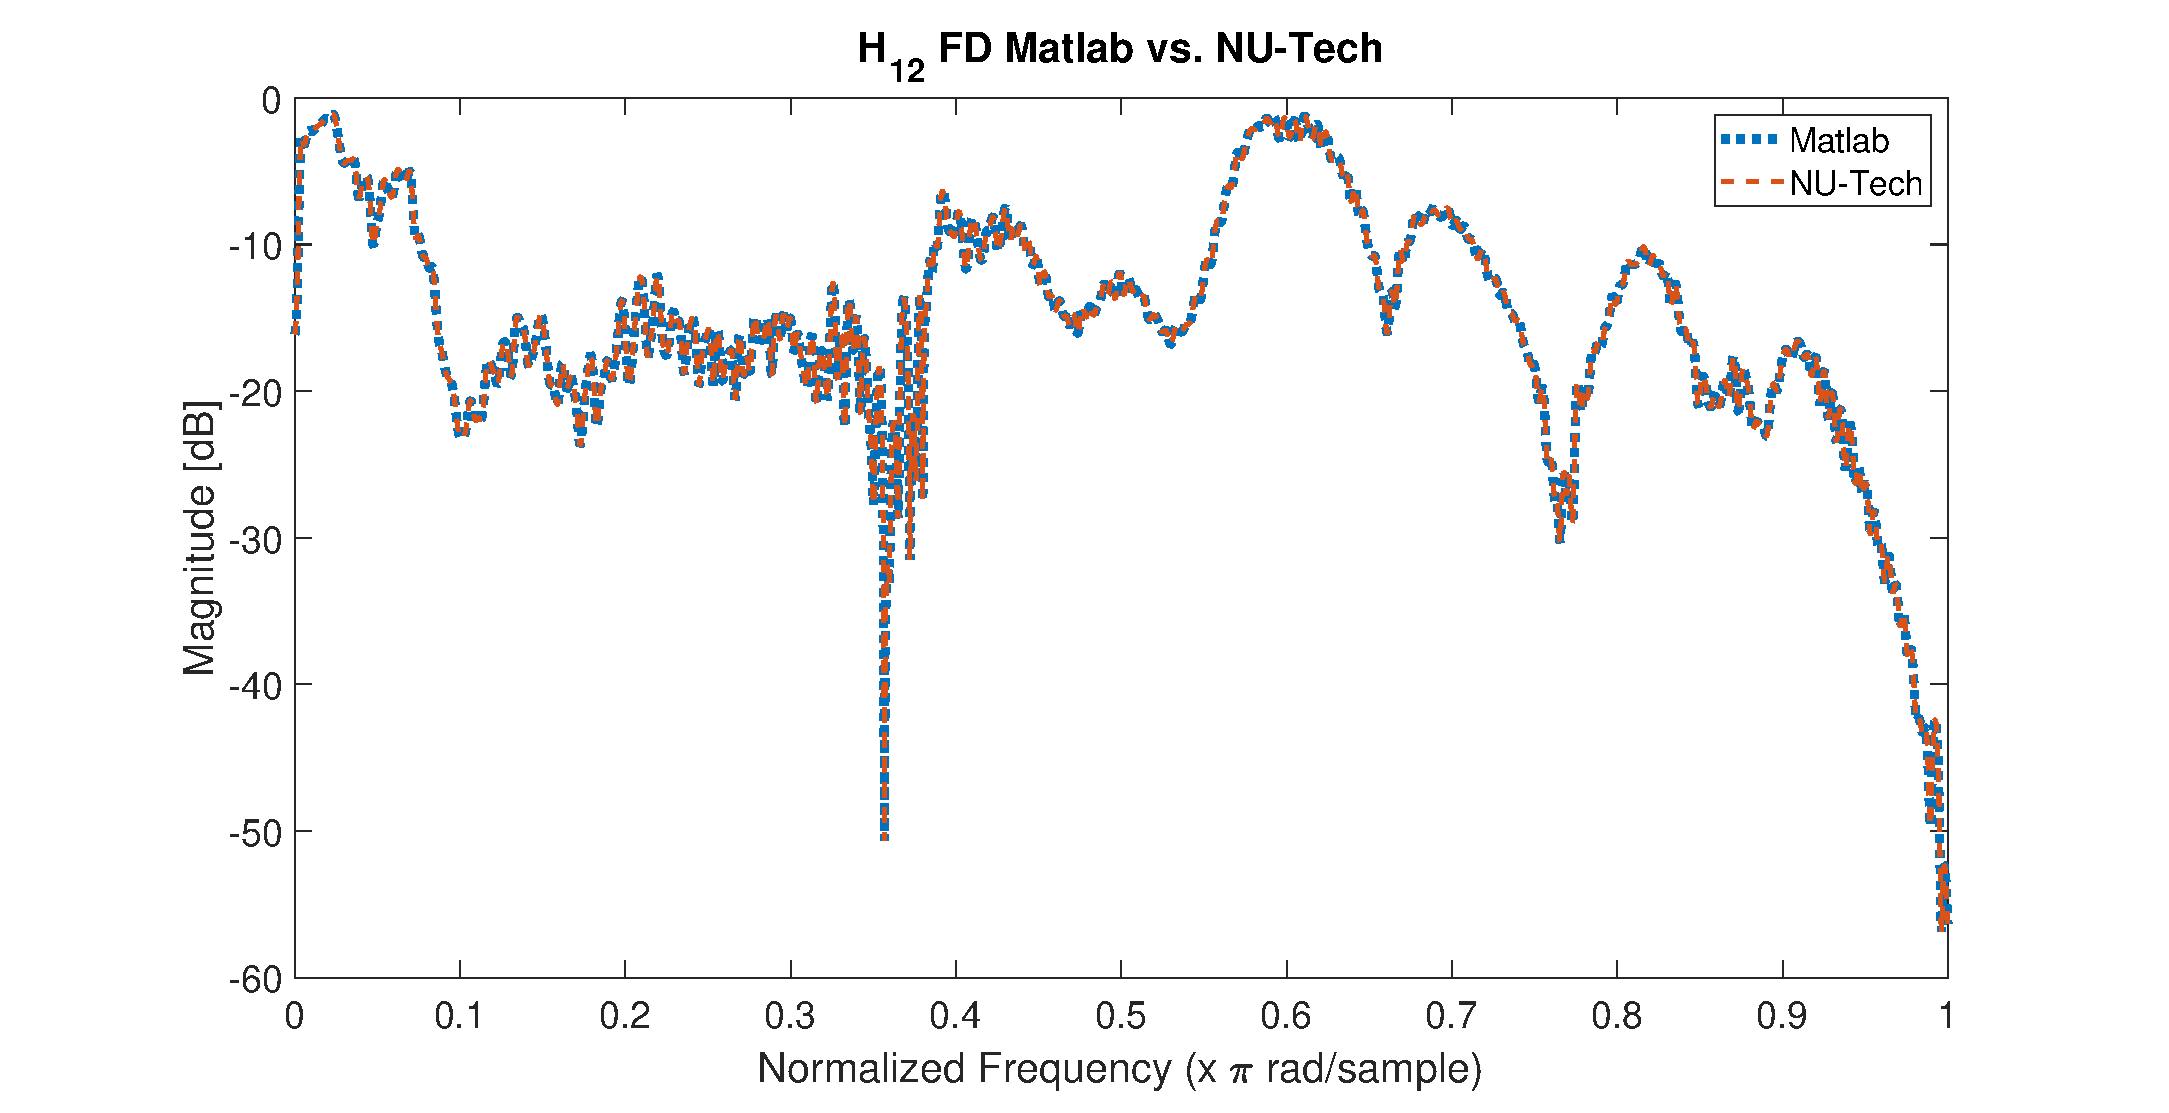
\includegraphics[width=1\textwidth]{Immagini/H12_FD_matlab_nutech}
			\caption{}
			\label{fig:H12_FD_matlab_nutech}
	\end{subfigure}
\end{figure}

\begin{figure}[h]
	\ContinuedFloat
	\centering
	\begin{subfigure}{1\textwidth}
		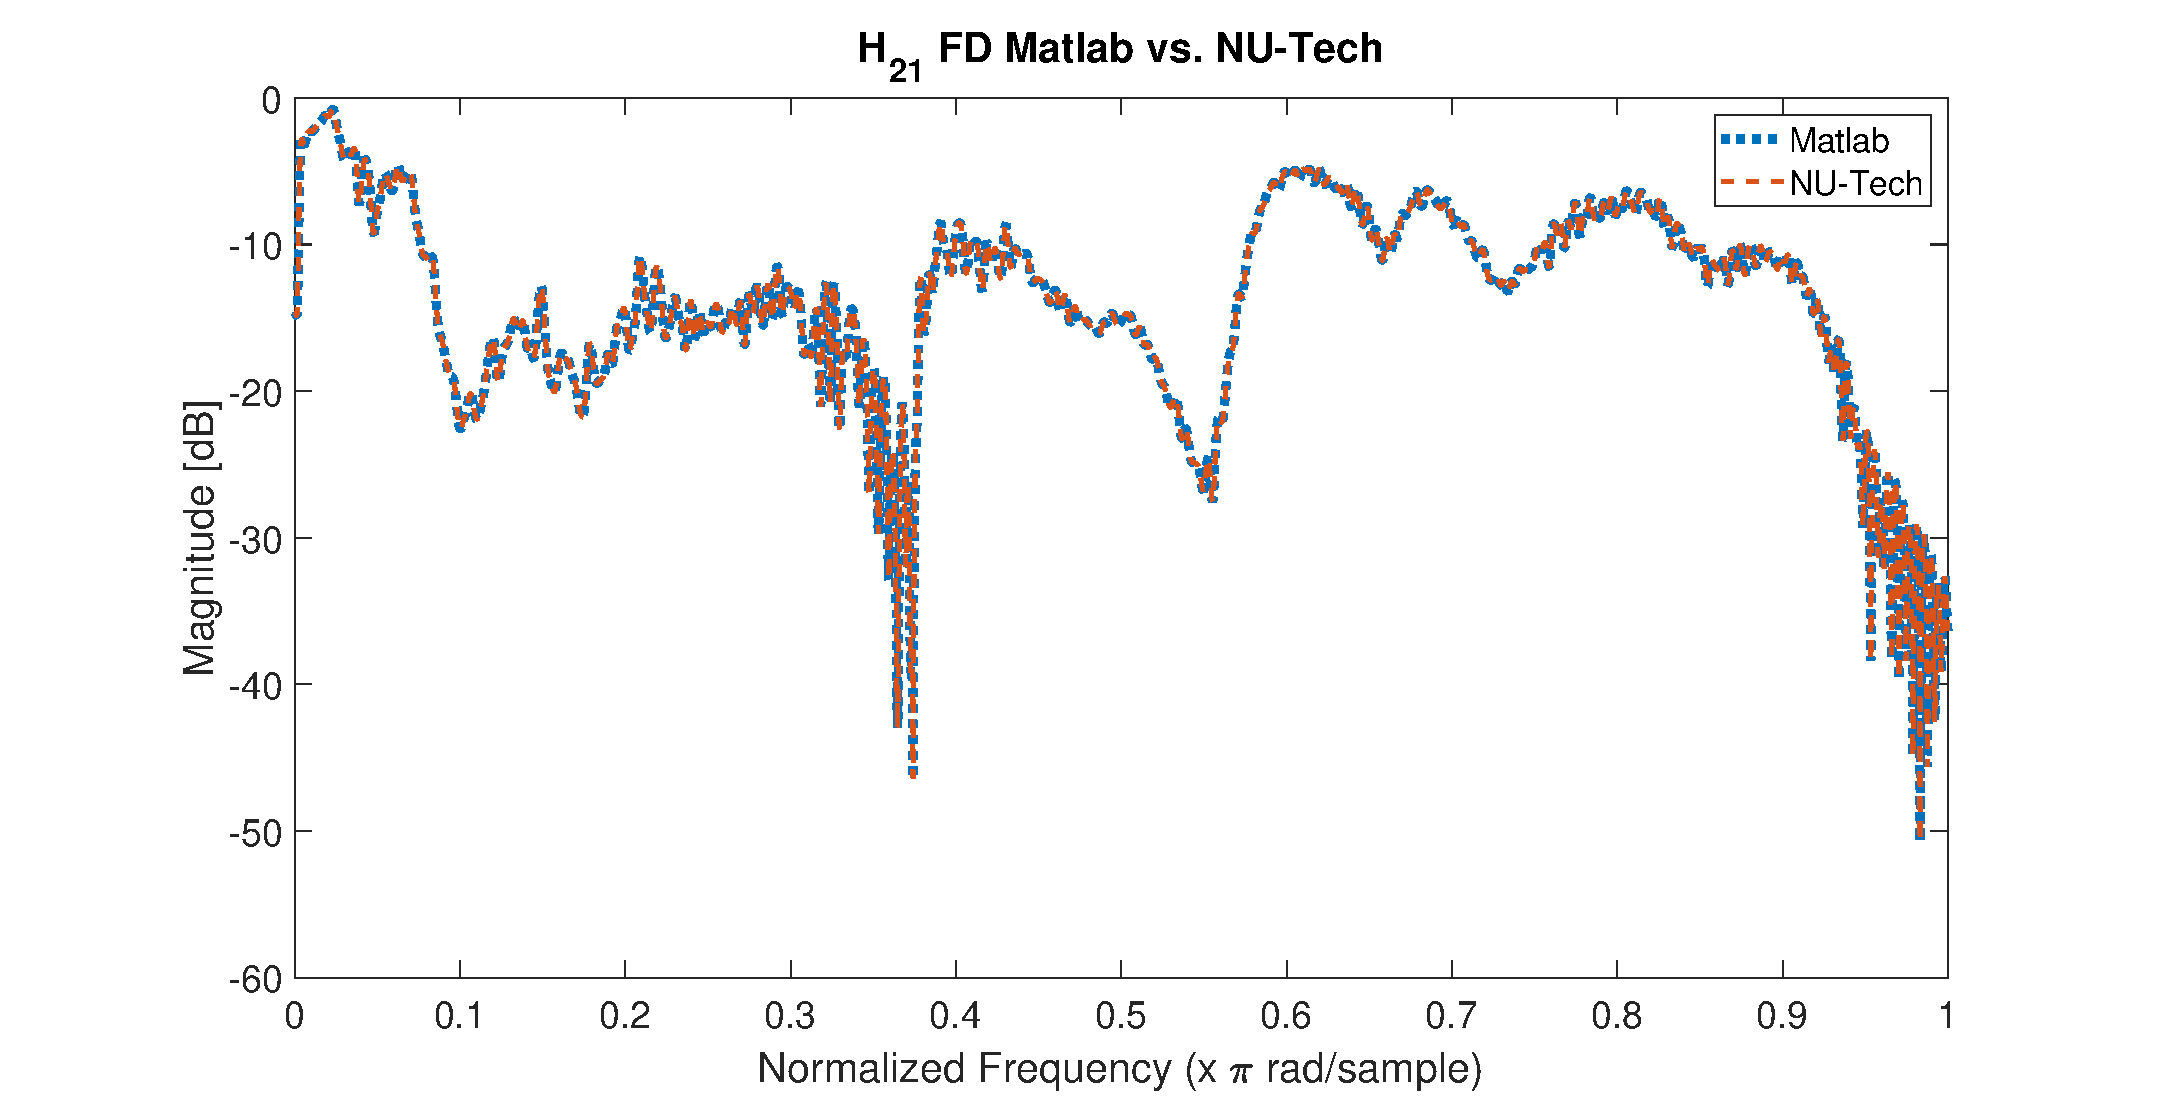
\includegraphics[width=1\textwidth]{Immagini/H21_FD_matlab_nutech}
		\caption{}
		\label{fig:H21_FD_matlab_nutech}
	\end{subfigure}\\
	\begin{subfigure}{1\textwidth}
		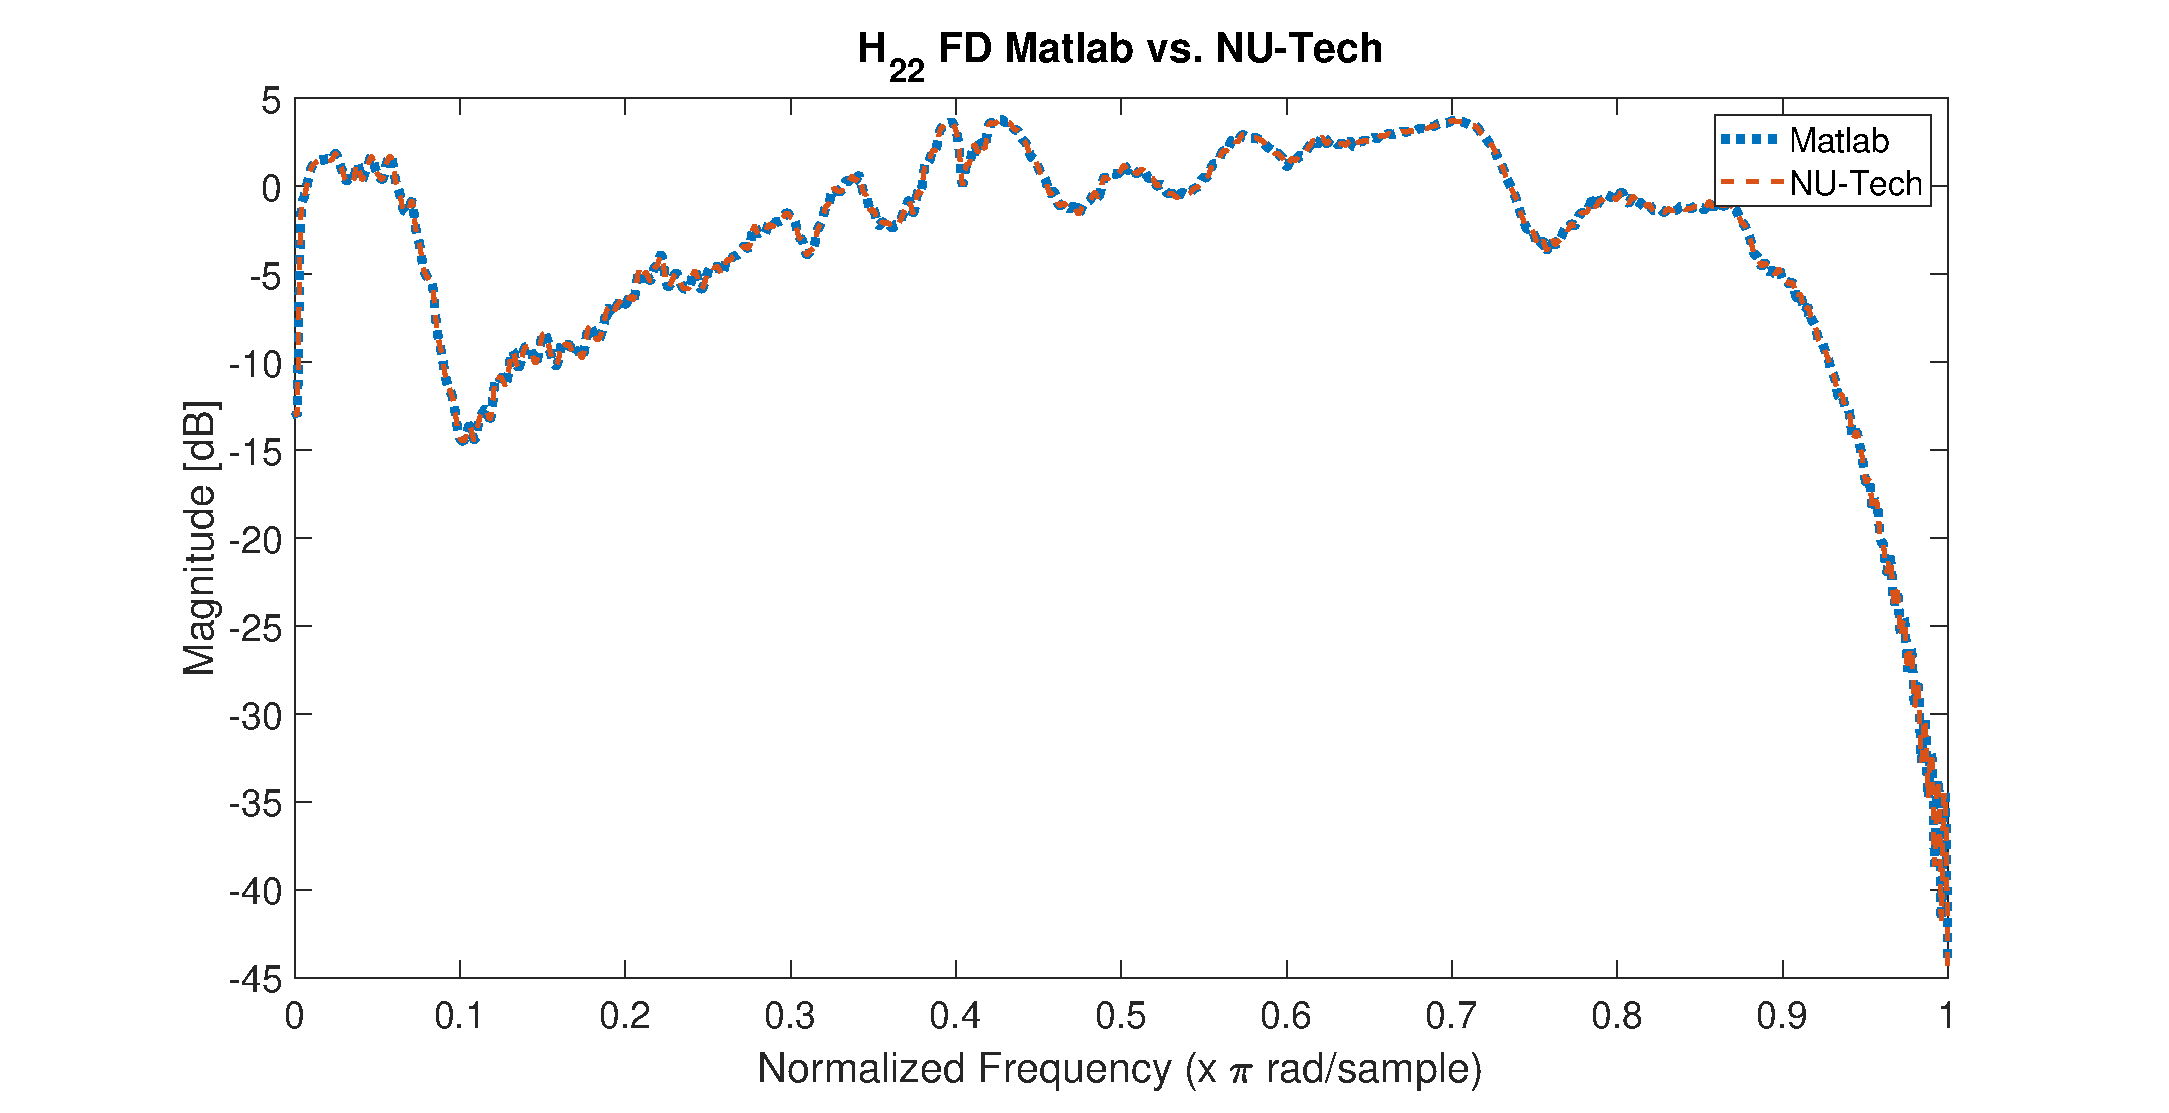
\includegraphics[width=1\textwidth]{Immagini/H22_FD_matlab_nutech}
		\caption{}
		\label{fig:H22_FD_matlab_nutech}
	\end{subfigure}
		\caption{Confronto dei filtri di cancellazione del crosstalk (a) $H_{11}$, (b) $H_{12}$, (c) $H_{21}$ e (d) $H_{22}$ in Matlab e in NU-Tech per l'algoritmo Fast Deconvolution.}
		\label{fig:confronto_filtri_matlab_nutech_fd}
\end{figure}

Dall'ascolto possiamo affermare che l'algoritmo migliore è il Fast Deconvolution poiché nello scenario ``statico'' in cui abbiamo lavorato, dato che in ingresso ad entrambi gli algoritmi abbiamo dato una canzone e delle HRTF precedentemente salvate, raggiunge subito la convergenza e si può notare una buona separazione dei due canali. L'algoritmo LMS, invece, poiché adattativo, ha necessità di un certo tempo prima che l'errore tra il segnale desiderato e l'uscita diventi minimo. Questo intervallo è udibile all'orecchio umano e l'ascoltatore potrebbe non sentire in modo fluido i primi istanti di riproduzione.

\clearpage

\section{Conclusioni}
\label{sec:conclusioni}
Lo scopo della tesina era quello di confrontare gli algoritmi LMS e Fast Deconvolution come nel paper~\cite{Li:comprehensive_comparison}. Per fare questo sono prima stati implementati gli algoritmi in Matlab verificando il corretto funzionamento tramite un confronto tra l'uscita e l'ingresso. Notando quindi che l'uscita segue l'ingresso, si può affermare che nell'equazione~\eqref{eq:Y=CHX} la matrice $\mathbf{C}$ è uguale all'inversa di $\mathbf{H}$, dunque $\mathbf{C} = \mathbf{H}^{-1}$, dato che l'ingresso $\mathbf{X}$ è uguale all'uscita $\mathbf{Y}$, cioè $\mathbf{Y} = \mathbf{X}$.

Dato che il programma in Matlab funziona correttamente, si è passato all'implementazione in NU-Tech. Lo sviluppo in Matlab è stato necessario in quanto è un linguaggio ad alto livello e più semplice di C++, questo ci ha permesso di scrivere i programmi in modo più semplice e veloce e di avere dei risultati di riferimento con cui confrontare le uscite prodotte dal NUTS.

Grazie al programma NU-Tech abbiamo sviluppato due NUTS che svolgono gli algoritmi LMS e Fast Deconvolution. Sono inoltre state inserite due funzionalità, cioè quella di permettere all'utente di cambiare dalla board NU-Tech il percorso in cui sono salvate le HRTF e i parametri $\beta$ e $\mu$ che vanno a influire sulla prestazioni dei due algoritmi. Queste funzionalità sono utili all'ascoltatore che non deve conosce nessun linguaggio di programmazione per modificare questi parametri, basta semplicemente usare l'interfaccia grafica messa a disposizione.

I risultati oggettivi ottenuti, cioè il calcolo dei fattori di separazione dei canali sono in linea con~\cite{Li:comprehensive_comparison} tranne per il fatto che il fattore di separazione del canale sinistro è migliore di quello destro, ma questo può essere dovuto alla diversa scelta del dataset delle HRTF.

Dall'ascolto possiamo affermare che l'algoritmo Fast Deconvolution è migliore rispetto a LMS, soprattutto perché riteniamo che l'intervallo di tempo in cui l'errore deve essere minimizzato nell'algoritmo adattativo possa essere fastidioso per l'ascoltatore. Quando l'algoritmo LMS è a regime non notiamo nessuna differenza con la Fast Deconvolution, nonostante i fattori di separazione dei canali hanno diversi decibel di differenza tra i due algoritmi.

Tra gli sviluppi futuri si potrebbero prendere in considerazione dei test soggettivi più accurati. In condizioni più professionali la percezione dell'audio potrebbe cambiare all'ascolto di persone con un udito più sensibile. Si potrebbe affiancare agli algoritmi di cancellazione del crosstalk un programma che monitora la posizione della testa dell'ascoltatore e modella la stanza in cui si trova~\cite{Bai:objective_analysis}. Dai test soggettivi, questo sistema audio interattivo mostra che la percezione del suono migliora notevolmente. Usando questo sistema, le HRTF non saranno più fisse, ma varieranno a seconda della posizione dell'ascoltatore nella stanza.

%Nelle conclusioni dovete rispiegare brevemente lo scopo della tesina e quello che è stato fatto (che i due algoritmi sono stati implementati prima in matlab e poi in nutech), sintetizzare i risultati che sono stati ottenuti comparati con lo stato dell'arte (non c'è bisogno di fare riferimento a tabelle e figure) e descrivere quali potrebbero essere gli sviluppi futuri (ad esempio svolgere dei test soggettivi formali più approfonditi e misurare direttamente le HRTF considerando il set-up che poi verrà utilizzato per gli esperimenti)

%Dai risultati mostrati nel capitolo~\ref{sec:risultati}, si possono fare diverse osservazioni. Si può notare dalla figura~\ref{fig:channel_separation_LMS_FD} che nel fattore di separazione dei canali il numeratore è quasi sempre maggiore del denominatore: questo indica che la separazione dei canali sta avvenendo in modo corretto. 

%Si può osservare dalla figura~\ref{fig:mse_LMS} che all'aumentare del tempo l'errore dell'algorimo LMS diminuisce: questo indica che l'algoritmo produrrà un'uscita sempre più vicina a quella desiderata. 

%Dalla figura~\ref{fig:confronto_H_LMS_FD} si nota che i filtri $H_{11}$ e $H_{22}$ trovati con LMS e FD sono più simili tra loro rispetto ai filtri $H_{12}$ e $H_{21}$.

%Si può notare dalla tabella~\ref{tab:LMS_result} che il fattore di separazione dei canali aumenta all'aumentare di $\mu$, mentre per la tabella~\ref{tab:FD_result} questo fattore aumenta al diminuire di $\beta$. Entrambi i parametri vengono aggiustati durante l'implementazione pratica, in particolare, il comportamento del $\beta$ per la Fast Deconvolution è in linea con quanto ci si aspetta dalla formula~\eqref{eq:funzione_costo_fd} spiegata nel capitolo~\ref{subsec:FD_teoria}.

%A differenza del paper di riferimento~\cite{Li:comprehensive_comparison}, in cui il fattore di separazione dei canali è migliore per il canale destro, nel nostro caso otteniamo valori migliori per il canale sinistro. Questo può essere dovuto ad una diversa scelta delle HRIR tra l'implementazione dell'articolo e la nostra. Nelle simulazioni dell'articolo, infatti, è stato utilizzato il valore medio di 10 set di HRTF per calcolare la matrice di cancellazione della diafonia $H$, e successivamente sono stati utilizzati i 10 set originali di HRTF per calcolare i rispettivamente fattori di separazione dei canali.

%Dalle tabelle~\ref{tab:LMS_result} e~\ref{tab:FD_result} si ottengono dei fattori di separazione dei molto simili a quelli proposti in~\cite{Li:comprehensive_comparison}, in cui si ha in media $J_L = \SI{12.6251}{\decibel}$ e $J_R = \SI{16.0611}{\decibel}$ per LMS e $J_L = \SI{12.8147}{\decibel}$ e $J_R = \SI{17.2171}{\decibel}$ per FD. Possiamo dunque affermare che i filtri di cancellazione del crosstalk lavorano in modo corretto.

%Dal confronto tra l'uscita desiderata e l'ingresso in figura~\ref{fig:confronto_ingressi_uscite_LMS_FD} si può notare come questi segnali siano sovrapposti: possiamo sostenere dunque che la cancellazione del crosstalk avviene in modo corretto.

%I risultati ottenuti per ognuno dei due algoritmi con il Nu-Tech sono uguali a quelli prodotti dal Matlab, questo ci permette di affermare che gli algoritmi sviluppati nei due diversi linguaggi di programmazione sono equivalenti e producono le stesse uscite.

\clearpage 
\nocite{*}
%Il comando \printbibliography produce la sezione bibliografica con relativi
%titolo e testatina. Per mandarne il relativo titolo nell’indice generale si
%usa l’istruzione:
\printbibliography

\end{document} 